% Options for packages loaded elsewhere
\PassOptionsToPackage{unicode}{hyperref}
\PassOptionsToPackage{hyphens}{url}
\PassOptionsToPackage{dvipsnames,svgnames,x11names}{xcolor}
%
\documentclass[
  letterpaper,
  DIV=11,
  numbers=noendperiod]{scrreprt}

\usepackage{amsmath,amssymb}
\usepackage{iftex}
\ifPDFTeX
  \usepackage[T1]{fontenc}
  \usepackage[utf8]{inputenc}
  \usepackage{textcomp} % provide euro and other symbols
\else % if luatex or xetex
  \usepackage{unicode-math}
  \defaultfontfeatures{Scale=MatchLowercase}
  \defaultfontfeatures[\rmfamily]{Ligatures=TeX,Scale=1}
\fi
\usepackage{lmodern}
\ifPDFTeX\else  
    % xetex/luatex font selection
\fi
% Use upquote if available, for straight quotes in verbatim environments
\IfFileExists{upquote.sty}{\usepackage{upquote}}{}
\IfFileExists{microtype.sty}{% use microtype if available
  \usepackage[]{microtype}
  \UseMicrotypeSet[protrusion]{basicmath} % disable protrusion for tt fonts
}{}
\makeatletter
\@ifundefined{KOMAClassName}{% if non-KOMA class
  \IfFileExists{parskip.sty}{%
    \usepackage{parskip}
  }{% else
    \setlength{\parindent}{0pt}
    \setlength{\parskip}{6pt plus 2pt minus 1pt}}
}{% if KOMA class
  \KOMAoptions{parskip=half}}
\makeatother
\usepackage{xcolor}
\setlength{\emergencystretch}{3em} % prevent overfull lines
\setcounter{secnumdepth}{5}
% Make \paragraph and \subparagraph free-standing
\makeatletter
\ifx\paragraph\undefined\else
  \let\oldparagraph\paragraph
  \renewcommand{\paragraph}{
    \@ifstar
      \xxxParagraphStar
      \xxxParagraphNoStar
  }
  \newcommand{\xxxParagraphStar}[1]{\oldparagraph*{#1}\mbox{}}
  \newcommand{\xxxParagraphNoStar}[1]{\oldparagraph{#1}\mbox{}}
\fi
\ifx\subparagraph\undefined\else
  \let\oldsubparagraph\subparagraph
  \renewcommand{\subparagraph}{
    \@ifstar
      \xxxSubParagraphStar
      \xxxSubParagraphNoStar
  }
  \newcommand{\xxxSubParagraphStar}[1]{\oldsubparagraph*{#1}\mbox{}}
  \newcommand{\xxxSubParagraphNoStar}[1]{\oldsubparagraph{#1}\mbox{}}
\fi
\makeatother

\usepackage{color}
\usepackage{fancyvrb}
\newcommand{\VerbBar}{|}
\newcommand{\VERB}{\Verb[commandchars=\\\{\}]}
\DefineVerbatimEnvironment{Highlighting}{Verbatim}{commandchars=\\\{\}}
% Add ',fontsize=\small' for more characters per line
\usepackage{framed}
\definecolor{shadecolor}{RGB}{241,243,245}
\newenvironment{Shaded}{\begin{snugshade}}{\end{snugshade}}
\newcommand{\AlertTok}[1]{\textcolor[rgb]{0.68,0.00,0.00}{#1}}
\newcommand{\AnnotationTok}[1]{\textcolor[rgb]{0.37,0.37,0.37}{#1}}
\newcommand{\AttributeTok}[1]{\textcolor[rgb]{0.40,0.45,0.13}{#1}}
\newcommand{\BaseNTok}[1]{\textcolor[rgb]{0.68,0.00,0.00}{#1}}
\newcommand{\BuiltInTok}[1]{\textcolor[rgb]{0.00,0.23,0.31}{#1}}
\newcommand{\CharTok}[1]{\textcolor[rgb]{0.13,0.47,0.30}{#1}}
\newcommand{\CommentTok}[1]{\textcolor[rgb]{0.37,0.37,0.37}{#1}}
\newcommand{\CommentVarTok}[1]{\textcolor[rgb]{0.37,0.37,0.37}{\textit{#1}}}
\newcommand{\ConstantTok}[1]{\textcolor[rgb]{0.56,0.35,0.01}{#1}}
\newcommand{\ControlFlowTok}[1]{\textcolor[rgb]{0.00,0.23,0.31}{\textbf{#1}}}
\newcommand{\DataTypeTok}[1]{\textcolor[rgb]{0.68,0.00,0.00}{#1}}
\newcommand{\DecValTok}[1]{\textcolor[rgb]{0.68,0.00,0.00}{#1}}
\newcommand{\DocumentationTok}[1]{\textcolor[rgb]{0.37,0.37,0.37}{\textit{#1}}}
\newcommand{\ErrorTok}[1]{\textcolor[rgb]{0.68,0.00,0.00}{#1}}
\newcommand{\ExtensionTok}[1]{\textcolor[rgb]{0.00,0.23,0.31}{#1}}
\newcommand{\FloatTok}[1]{\textcolor[rgb]{0.68,0.00,0.00}{#1}}
\newcommand{\FunctionTok}[1]{\textcolor[rgb]{0.28,0.35,0.67}{#1}}
\newcommand{\ImportTok}[1]{\textcolor[rgb]{0.00,0.46,0.62}{#1}}
\newcommand{\InformationTok}[1]{\textcolor[rgb]{0.37,0.37,0.37}{#1}}
\newcommand{\KeywordTok}[1]{\textcolor[rgb]{0.00,0.23,0.31}{\textbf{#1}}}
\newcommand{\NormalTok}[1]{\textcolor[rgb]{0.00,0.23,0.31}{#1}}
\newcommand{\OperatorTok}[1]{\textcolor[rgb]{0.37,0.37,0.37}{#1}}
\newcommand{\OtherTok}[1]{\textcolor[rgb]{0.00,0.23,0.31}{#1}}
\newcommand{\PreprocessorTok}[1]{\textcolor[rgb]{0.68,0.00,0.00}{#1}}
\newcommand{\RegionMarkerTok}[1]{\textcolor[rgb]{0.00,0.23,0.31}{#1}}
\newcommand{\SpecialCharTok}[1]{\textcolor[rgb]{0.37,0.37,0.37}{#1}}
\newcommand{\SpecialStringTok}[1]{\textcolor[rgb]{0.13,0.47,0.30}{#1}}
\newcommand{\StringTok}[1]{\textcolor[rgb]{0.13,0.47,0.30}{#1}}
\newcommand{\VariableTok}[1]{\textcolor[rgb]{0.07,0.07,0.07}{#1}}
\newcommand{\VerbatimStringTok}[1]{\textcolor[rgb]{0.13,0.47,0.30}{#1}}
\newcommand{\WarningTok}[1]{\textcolor[rgb]{0.37,0.37,0.37}{\textit{#1}}}

\providecommand{\tightlist}{%
  \setlength{\itemsep}{0pt}\setlength{\parskip}{0pt}}\usepackage{longtable,booktabs,array}
\usepackage{calc} % for calculating minipage widths
% Correct order of tables after \paragraph or \subparagraph
\usepackage{etoolbox}
\makeatletter
\patchcmd\longtable{\par}{\if@noskipsec\mbox{}\fi\par}{}{}
\makeatother
% Allow footnotes in longtable head/foot
\IfFileExists{footnotehyper.sty}{\usepackage{footnotehyper}}{\usepackage{footnote}}
\makesavenoteenv{longtable}
\usepackage{graphicx}
\makeatletter
\def\maxwidth{\ifdim\Gin@nat@width>\linewidth\linewidth\else\Gin@nat@width\fi}
\def\maxheight{\ifdim\Gin@nat@height>\textheight\textheight\else\Gin@nat@height\fi}
\makeatother
% Scale images if necessary, so that they will not overflow the page
% margins by default, and it is still possible to overwrite the defaults
% using explicit options in \includegraphics[width, height, ...]{}
\setkeys{Gin}{width=\maxwidth,height=\maxheight,keepaspectratio}
% Set default figure placement to htbp
\makeatletter
\def\fps@figure{htbp}
\makeatother
% definitions for citeproc citations
\NewDocumentCommand\citeproctext{}{}
\NewDocumentCommand\citeproc{mm}{%
  \begingroup\def\citeproctext{#2}\cite{#1}\endgroup}
\makeatletter
 % allow citations to break across lines
 \let\@cite@ofmt\@firstofone
 % avoid brackets around text for \cite:
 \def\@biblabel#1{}
 \def\@cite#1#2{{#1\if@tempswa , #2\fi}}
\makeatother
\newlength{\cslhangindent}
\setlength{\cslhangindent}{1.5em}
\newlength{\csllabelwidth}
\setlength{\csllabelwidth}{3em}
\newenvironment{CSLReferences}[2] % #1 hanging-indent, #2 entry-spacing
 {\begin{list}{}{%
  \setlength{\itemindent}{0pt}
  \setlength{\leftmargin}{0pt}
  \setlength{\parsep}{0pt}
  % turn on hanging indent if param 1 is 1
  \ifodd #1
   \setlength{\leftmargin}{\cslhangindent}
   \setlength{\itemindent}{-1\cslhangindent}
  \fi
  % set entry spacing
  \setlength{\itemsep}{#2\baselineskip}}}
 {\end{list}}
\usepackage{calc}
\newcommand{\CSLBlock}[1]{\hfill\break\parbox[t]{\linewidth}{\strut\ignorespaces#1\strut}}
\newcommand{\CSLLeftMargin}[1]{\parbox[t]{\csllabelwidth}{\strut#1\strut}}
\newcommand{\CSLRightInline}[1]{\parbox[t]{\linewidth - \csllabelwidth}{\strut#1\strut}}
\newcommand{\CSLIndent}[1]{\hspace{\cslhangindent}#1}

\KOMAoption{captions}{tableheading}
\makeatletter
\@ifpackageloaded{bookmark}{}{\usepackage{bookmark}}
\makeatother
\makeatletter
\@ifpackageloaded{caption}{}{\usepackage{caption}}
\AtBeginDocument{%
\ifdefined\contentsname
  \renewcommand*\contentsname{Table of contents}
\else
  \newcommand\contentsname{Table of contents}
\fi
\ifdefined\listfigurename
  \renewcommand*\listfigurename{List of Figures}
\else
  \newcommand\listfigurename{List of Figures}
\fi
\ifdefined\listtablename
  \renewcommand*\listtablename{List of Tables}
\else
  \newcommand\listtablename{List of Tables}
\fi
\ifdefined\figurename
  \renewcommand*\figurename{Figure}
\else
  \newcommand\figurename{Figure}
\fi
\ifdefined\tablename
  \renewcommand*\tablename{Table}
\else
  \newcommand\tablename{Table}
\fi
}
\@ifpackageloaded{float}{}{\usepackage{float}}
\floatstyle{ruled}
\@ifundefined{c@chapter}{\newfloat{codelisting}{h}{lop}}{\newfloat{codelisting}{h}{lop}[chapter]}
\floatname{codelisting}{Listing}
\newcommand*\listoflistings{\listof{codelisting}{List of Listings}}
\makeatother
\makeatletter
\makeatother
\makeatletter
\@ifpackageloaded{caption}{}{\usepackage{caption}}
\@ifpackageloaded{subcaption}{}{\usepackage{subcaption}}
\makeatother

\ifLuaTeX
  \usepackage{selnolig}  % disable illegal ligatures
\fi
\usepackage{bookmark}

\IfFileExists{xurl.sty}{\usepackage{xurl}}{} % add URL line breaks if available
\urlstyle{same} % disable monospaced font for URLs
\hypersetup{
  pdftitle={Research Project on SSAO Extraction and Enzyme Kinetics},
  pdfauthor={Prasaath Sastha Kuppan Ravi},
  colorlinks=true,
  linkcolor={blue},
  filecolor={Maroon},
  citecolor={Blue},
  urlcolor={Blue},
  pdfcreator={LaTeX via pandoc}}


\title{Research Project on SSAO Extraction and Enzyme Kinetics}
\author{Prasaath Sastha Kuppan Ravi}
\date{}

\begin{document}
\maketitle

\renewcommand*\contentsname{Table of contents}
{
\hypersetup{linkcolor=}
\setcounter{tocdepth}{2}
\tableofcontents
}

\bookmarksetup{startatroot}

\chapter*{Preface}\label{preface}
\addcontentsline{toc}{chapter}{Preface}

\markboth{Preface}{Preface}

\textbf{Overview}

This is a research project carried out at the University of
Hertfordshire in compliance with its regulations under the supervision
of Dr.~John Skamarauskas. The project was submitted in partial
fulfillment of my Master's in Drug Discovery and Toxicology. The
original submission was prepared in Microsoft word, and the data
analysis was carried performed using Graphpad prism.

This version of the project published as a quarto book is purely an
exploratory effort by me. Same data from original research was used, and
R was used to generate plots, models and tables. The results obtained
from the R code was compared with the original results from Graphpad
which were identical. I decided to do this to improve my working
understanding of R and Quarto Markdown.

\section*{\texorpdfstring{\textbf{Abstract}}{Abstract}}\label{abstract}
\addcontentsline{toc}{section}{\textbf{Abstract}}

\markright{\textbf{Abstract}}

Rat brown adipose tissue (BAT) is recognized as a rich source of semi
carbazide-sensitive amine oxidase (SSAO), yet no standardized methods
for extracting SSAO from rat BAT have been published. This study aims to
develop and optimize a robust methodology for SSAO extraction from rat
BAT and to investigate its enzymatic kinetics using benzylamine as a
substrate. The study involved comparing different extraction methods,
quantifying the extracted protein using Bradford and BCA assays, and
assessing SSAO activity through the Amplex\textsuperscript{®} Red
monoamine oxidase assay.

The kinetic parameters of SSAO were determined, with a Km value of
0.03193mM for benzylamine, closely aligning with literature under
similar experimental conditions. Furthermore, the inhibitory effects of
caffeine and simvastatin on SSAO activity were evaluated, although, the
Ki values obtained were based on a single experiment, leading to wider
error margins and lower confidence.

This research provides a detailed methodology for SSAO extraction from
rat BAT, confirming that proteins can be successfully extracted and that
SSAO activity remains quantifiable post-extraction. However, further
studies with improved experimental controls are recommended to refine
the inhibitory kinetics of caffeine and simvastatin on SSAO.

\section*{\texorpdfstring{\textbf{Abbreviations}}{Abbreviations}}\label{abbreviations}
\addcontentsline{toc}{section}{\textbf{Abbreviations}}

\markright{\textbf{Abbreviations}}

\begin{longtable}[]{@{}l@{}}
\toprule\noalign{}
\endhead
\bottomrule\noalign{}
\endlastfoot
BAT - Brown Adipose Tissue \\
BCA - Bicinchoninic Acid \\
BSA - Bovine Serum Albumin \\
CAF - Caffeine \\
Ki - Inhibition Constant \\
Km - Michaelis Menten Constant \\
SIM - Simvastatin \\
SSAO - Semi Carbazide Sensitive Amine Oxidase \\
V0 - Initial Velocity \\
VAP-1 - Vascular Adhesion Protein 1 \\
Vmax - Maximum Velocity \\
HRP - Horseradish Peroxidase \\
EtOH - Ethanol \\
SEM - Standard Error in Mean \\
MAO A - Monoamine Oxidase A \\
MAO B - Monoamine Oxidase B \\
AOC - Amine Oxidase Copper-Containing \\
dH20 - Deionised Water \\
ReLi - Removal of Excess Lipids \\
CST - Cell Signalling Technologies -- Commercial kit. \\
DMSO - Dimethyl Sulfoxide \\
\end{longtable}

\bookmarksetup{startatroot}

\chapter{Introduction}\label{introduction}

\section{\texorpdfstring{\textbf{Amine Oxidases and
substrates}}{Amine Oxidases and substrates}}\label{amine-oxidases-and-substrates}

Amine oxidases are a common group of copper containing enzymes highly
expressed in smooth muscle cells, vascular endothelial cells and
adipocytes in humans and rats (Manasieva et al. 2022; Salmi, Tohka, and
Jalkanen 2000; Salmi and Jalkanen 1992). The key enzymatic function of
these proteins is oxidating primary amines into aldehydes . This also
results in formation of byproducts such as ammonium
(NH\textsubscript{4}\textsuperscript{+}) and hydrogen
peroxide(H\textsubscript{2}O\textsubscript{2}) in a two-step reaction
Figure~\ref{fig-Deamination_of_primaryamine_SSAO} . (Salmi and Jalkanen
2019)

\begin{fig}

\centering{

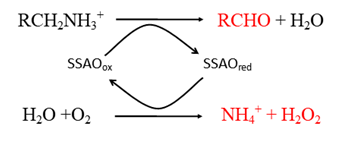
\includegraphics[width=2.88542in,height=\textheight]{images/clipboard-4135545146.png}

}

\caption{\label{fig-Deamination_of_primaryamine_SSAO}Deamination of a
primary amine by SSAO to form an aldehyde, ammonium, and hydrogen
peroxide in a 2-step reaction.}

\end{fig}%

Semi carbazide sensitive amine oxidase (SSAO) also known as the vascular
adhesion protein belongs to this class of enzymes and are primarily
present on the epithelial cell membranes of the vascular surfaces. Some
of the known forms of SSAO enzymes in humans are AOC1, AOC2, and AOC3.
AOC1 is involved in regulating histaminase, whereas AOC2 and AOC3
(VAP-1) catalyse various monoamines. AOC2 has a large substrate channel
compared to the AOC3. The preferred substrates for AOC2 are ethylamine,
tyramine, and p-tyramine, whereas AOC3 or VAP 1 prefers methylamine
(Salmi and Jalkanen 2019). Benzylamine is a xenobiotic substrate of
AOC-3 or VAP1 and is more commonly used in invitro studies of SSAO
kinetics and VAP 1 contributes to approximately 90\% of cellular SSAO
activity in mammals (Salmi and Jalkanen 2019) . Other synthetic
substrates such as aminoacetone, allylamine, and methylamine are also
used in invitro experiments (Maria Carmen Iglesias-Osma et al. 2005;
Lyles 1995; Manasieva et al. 2023, 2022). This project studies the
activity of SSAO using benzylamine as the only substrate as it is
specific to SSAO and no other mono amine oxidases (MAO).

\section{\texorpdfstring{\textbf{SSAO/VAP1 Physiology and
Pathophysiology}}{SSAO/VAP1 Physiology and Pathophysiology}}\label{ssaovap1-physiology-and-pathophysiology}

The primary role of SSAO as an enzyme is catalysing primary amines that
are present in the circulation into aldehydes and hydrogen peroxide.
However, their expression and activity has been found to be upregulated
by inflammatory and immune mediators such as IL-1, TNF-α, and other
lipopolysaccharides in an organ culture study using human tonsillar
tissue (Arvilommi, Salmi, and Jalkanen 1997). The study also reported
that there is no significant difference in the characteristics of VAP-1
induced by inflammatory mediators and the naturally occurring VAP-1.
Studies have also shown that VAP-1 directly regulates lymphocytes /
leukocytes rolling under a defined laminar shear supporting the
lymphocyte extravasation process (Salmi, Tohka, and Jalkanen 2000). This
increases the understanding on VAP-1 expression and the outcomes of its
enzymatic activity on physiology and pathophysiology. The resulting
products of SSAO activity are aldehydes and hydrogen peroxides which are
implicated in development of various pathologic complications that
include atherosclerosis, diabetes, and obesity (Murata et al. 2017; Wang
et al. 2018). The extravasation cascade of leukocytes influenced by
VAP-1 is defined as a key point in development of various pathologies
such as Fibrosis, inflammation, ischemia reperfusion injury, and even
cancer (Salmi, Tohka, and Jalkanen 2000). Most of these effects were
studied by blocking the activity of VAP-1 using SSAO inhibitors
(Danielli et al. 2022; H. Li et al. 2021; Wang et al. 2018). VAP-1 is
also found in circulation / serum with almost the same characteristics
of the transmembrane bound VAP-1. Studies have reported that the levels
of serum VAP-1 is increased with pathologies such as colorectal cancer,
chronic liver disease, gastric cancer, inflammation, smoking, and aging
(Kurkijarvi et al. 2000; Pannecoeck et al. 2015; Toiyama et al. 2009;
Yasuda et al. 2011).

\section{\texorpdfstring{\textbf{SSAO in metabolic
disorders}}{SSAO in metabolic disorders}}\label{ssao-in-metabolic-disorders}

Recent trends in metabolic health have shown that obesity, diabetes, and
cardiovascular diseases are the leading causes of morbidity and loss of
quality of life (Chew et al. 2023). This makes it one of the growing
health concerns for every major health care organisation and insurance
companies.

\begin{figure}

\centering{

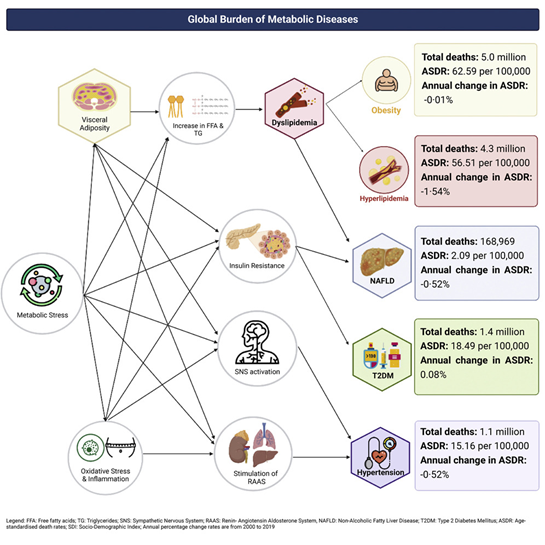
\includegraphics{images/clipboard-444669600.png}

}

\caption{\label{fig-DALY}Global burden of metabolic diseases portraying
various factors that lead to metabolic diseases causing increase in
morbidity and disability adjusted life years (DALYs)}

\end{figure}%

Figure~\ref{fig-DALY} provides a comprehensive overview of the several
factors leading to fatal metabolic disorders such as obesity,
hyperlipidemia, non-alcoholic fatty liver disease (NAFLD), type 2
diabetes mellitus, and hypertension.

Circulating SSAO is implicated in the pathogenesis of metabolic
disorders such as obesity, atherosclerosis, and diabetes mellitus by
promoting weight gain by producing an insulin like action (Zorzano et
al. 2003). Higher levels of SSAO in humans have been reported in various
metabolic and cardiovascular conditions like stroke, myocardial
infarction, atherosclerosis, diabetes, and obesity (Boomsma et al. 2000;
Bour et al. 2009; Sun et al. 2018; Unzeta et al. 2021). The list of
studies looking at SSAO as a target for management of cardiovascular and
metabolic diseases provides conclusive evidence of the role SSAO plays
in their pathogenesis (Abella et al. 2003; Boomsma et al. 2000; Jarnicki
et al. 2016; Obata 2006; Papukashvili, Rcheulishvili, and Deng 2020;
Schilter et al. 2015; Tábi et al. 2013; Unzeta et al. 2021; Yan et al.
2023; P. H. Yu and Deng 1998).

\section{\texorpdfstring{\textbf{Adipose
Tissue}}{Adipose Tissue}}\label{adipose-tissue}

Adipose tissue is an essential part of the mammalian lipid metabolism
which is used to store the excess lipids as triglycerides and aiding the
body to use them as fatty acids in between meals (Börgeson, Boucher, and
Hagberg 2022). In metabolic aberrations, the function of the adipose
tissues is compromised resulting in excess circulating lipids and fat
deposition in peripheral organs leading to metabolic diseases such as
diabetes, atherosclerosis, obesity, and fatty liver disease (Belligoli
et al. 2019; Chait and Hartigh 2020; Chusyd et al. 2016). White adipose
tissue (WAT) and brown adipose tissue (BAT) are the two most common
types of adipose tissues present in mammals. White adipose tissue
primarily stores the excess lipids and releases when the body needs it.
BAT, in addition to storing the excess lipids they are also involved in
thermogenesis in mice, rats, and humans Börgeson, Boucher, and Hagberg
(2022).

The adipose tissues express a wide range of proteins that include amine
oxidases such as the SSAOs (BARRAND et al., 1984; Barrant \& Callingham,
1984). Both WAT and BAT higher levels of SSAO which plays a key role in
activation of glucose transport and prevention of lipolysis in both
humans and rodents (Zorzano et al. 2003).

This project is aimed at successfully extracting SSAO from rat brown
adipose tissue by a suitable methodology. A major barrier in using
adipose tissue is the quantity of lipids present in the adipose tissues.
Brown adipose tissue from rats is chosen to be the source of the enzyme
for the following reasons.

\begin{enumerate}
\def\labelenumi{\arabic{enumi}.}
\tightlist
\item
  Previous studies involving the use of adipose tissue for extraction of
  proteins have been reported in the literature. These reports also
  provide the protocol for a successful removal of fat and compares the
  results of protein extracted from WAT and BAT (Marin et al. 2019).
\item
  The chosen animal for this project is rat as they are more commonly
  used at the University of Hertfordshire. Since a wide range of tissues
  are being used for other experiments, use of adipose tissue from this
  animal will aid in the three Rs of animal research.
\item
  The quantity of BAT that can be extracted from rats are significantly
  more than mice.
\end{enumerate}

\section{\texorpdfstring{\textbf{Caffeine and
Simvastatin}}{Caffeine and Simvastatin}}\label{caffeine-and-simvastatin}

\textbf{\emph{Caffeine}} is an aromatic purine alkaloid from the
methylxanthine class compounds. Commonly used to increase alertness,
concentration, and improve energy levels. Additionally, caffeine is
shown to have various other health benefits such as neuroprotective,
hepatoprotective, weight loss, and physical performance improvements
owing to its antioxidant properties. Caffeine exhibits its antioxidant
properties by acting as a scavenger of free radicals and increasing the
concentration of endogenous antioxidants such as glutathione (GSH)
(Reddy et al. 2024).

Caffeine has gained some attention as it has been reported to aid in
weight loss by stimulating lipolysis, thermogenesis, appetite
suppression, and increased metabolic rate. These effects closely match
with observations when SSAO is inhibited by known inhibitors in various
studies (Che et al. 2012). This study aims to determine if caffeine
possess a quantifiable inhibitory effect on SSAO.

\textbf{\emph{Simvastatin}} is one of the common medications prescribed
to lower cholesterol levels and used as preventative therapeutic for
various cardiovascular and cerebrovascular conditions. A study by Sun et
al., reported that simvastatin blocks soluble SSAO/VAP1 release in
rabbit animal models of cerebral ischemia. However, this study does not
provide a more accurate estimate of in IC50 or the Ki for simvastatin on
SSAO but only discusses the reduction in SSAO release into the blood
plasma (Sun et al. 2018).

Studying the effects of caffeine and simvastatin on SSAO activity paves
direction for considering commonly used molecules in par with some of
the new chemical entities being studied for their inhibitory properties
on SSAO/VAP- 1.

\section{\texorpdfstring{\textbf{SSAO/VAP-1
Inhibitors}}{SSAO/VAP-1 Inhibitors}}\label{ssaovap-1-inhibitors}

Some of the most widely studied compounds with an inhibitory effect on
SSAO are small molecules that include hydrazines, benzylamides, vitamin
B1 derivatives, oxime based primary amine oxidase inhibitors and
peptides (Manasieva et al. 2022; Pannecoeck et al. 2015).

\begin{longtable}[]{@{}
  >{\raggedright\arraybackslash}p{(\columnwidth - 10\tabcolsep) * \real{0.1667}}
  >{\raggedright\arraybackslash}p{(\columnwidth - 10\tabcolsep) * \real{0.1667}}
  >{\raggedright\arraybackslash}p{(\columnwidth - 10\tabcolsep) * \real{0.1667}}
  >{\raggedright\arraybackslash}p{(\columnwidth - 10\tabcolsep) * \real{0.1667}}
  >{\raggedright\arraybackslash}p{(\columnwidth - 10\tabcolsep) * \real{0.1667}}
  >{\raggedright\arraybackslash}p{(\columnwidth - 10\tabcolsep) * \real{0.1667}}@{}}
\caption{Table of inhibitors containing the experimental models they
were tested on with key major effects and appropriate references. Table
directly incorporated from (H. Li et al. 2021)}\tabularnewline
\toprule\noalign{}
\begin{minipage}[b]{\linewidth}\raggedright
Name of SSAO/VAP-1 Inhibitors
\end{minipage} & \begin{minipage}[b]{\linewidth}\raggedright
Off Target
\end{minipage} & \begin{minipage}[b]{\linewidth}\raggedright
Model
\end{minipage} & \begin{minipage}[b]{\linewidth}\raggedright
Species
\end{minipage} & \begin{minipage}[b]{\linewidth}\raggedright
Major effects
\end{minipage} & \begin{minipage}[b]{\linewidth}\raggedright
References
\end{minipage} \\
\midrule\noalign{}
\endfirsthead
\toprule\noalign{}
\begin{minipage}[b]{\linewidth}\raggedright
Name of SSAO/VAP-1 Inhibitors
\end{minipage} & \begin{minipage}[b]{\linewidth}\raggedright
Off Target
\end{minipage} & \begin{minipage}[b]{\linewidth}\raggedright
Model
\end{minipage} & \begin{minipage}[b]{\linewidth}\raggedright
Species
\end{minipage} & \begin{minipage}[b]{\linewidth}\raggedright
Major effects
\end{minipage} & \begin{minipage}[b]{\linewidth}\raggedright
References
\end{minipage} \\
\midrule\noalign{}
\endhead
\bottomrule\noalign{}
\endlastfoot
\textbf{Allyl-amines} & & & & & \\
LJP-1586 & MAO-A/B & ICH, SAH, Atherosclerotic plaque & CD1 mice,
Sprague-Dawley rats, LDLr-/- ApoB100/100 mice & Improved neurological
scores. Improved neurological outcomes. & (Ma et al. 2011; Silvola et
al. 2016; Xu et al. 2014) \\
MDL-72974A & MAO-B & Atherosclerosis, Obesity & KKAy mice & Reduction of
weight gain and atherosclerotic lesions. Reduction of weight gain & (P.
Yu et al. 2002; Peter H. Yu et al. 2004) \\
PXS-4728A & / & Atherosclerosis & New Zealand white rabbits, Apo E-/-
mice & Reduction of weight gain and atherosclerotic plaques. Reduction
of atheroma and oxidative stress. & (Wang et al. 2018) \\
\textbf{Hydra-zines} & & & & & \\
Aminoguanidine & DAO & Atherosclerosis & KKAy mice & Reduction of weight
gain and atherosclerotic lesions. & (P. Yu et al. 2002) \\
Phenyl hydrazine & MAO-B & Obesity & Zucker rat & Reduction of weight
gain & (Carpéné et al. 2019) \\
SCZ & LO & Embolic stroke & Sprague-Dawley rats, LDLr-/- mice &
Reduction of the infarct volume. Decreased macrophages/increased SMC in
established lesions with/without lipid lowering. & (Hernandez-Guillamon
et al. 2010; Ma et al. 2011; Peng et al. 2016; Yang et al. 2011; Zhang
et al. 2016) \\
& & MI & Sprague-Dawley rats & Reduced infarction sizes & (Yang et al.
2011) \\
& & ICH & CD1 mice & Improved neurological scores & (Ma et al. 2011) \\
LJP-1207 & / & MI & Sprague-Dawley rats & Reduced infarction sizes &
(Yang et al. 2011) \\
Hydralazine & MAO-A/B & MI & Sprague-Dawley rats & Reduced infarction
sizes & (Yang et al. 2011) \\
\textbf{VAP-1 siRNA} & & ICH & CD1 mice & Improved neurological scores &
(Ma et al. 2011) \\
\end{longtable}

\emph{Note: All above inhibitors, except VAP-1 siRNA, are irreversible
inhibitors that bind to the topaquinone (TPQ) cofactor of VAP-1. MAO-A:
monoamine oxidase A; MAO-B: monoamine oxidase B; ICH: intracerebral
haemorrhage; SAH: subarachnoid haemorrhage; MI: myocardial infarction;
DAO: diamine oxidase; LO: Lysyl oxidase; SCZ: Semi carbazide.}

Two sides of SSAO action in adipocytes

\begin{enumerate}
\def\labelenumi{\arabic{enumi}.}
\tightlist
\item
  Studies have shown that benzylamine administration promoted a higher
  SSAO activity in diabetic, obese and high fat diet fed mice and
  rabbits and increases glucose uptake and prevents lipolysis caused by
  an insulin mimicking action by the deamination activity of SSAO. This
  caused an improvement in glucose tolerance due to insulin mimetic
  action by benzylamine oxidation (María Carmen Iglesias-Osma et al.
  2004; Zorzano et al. 2003).
\item
  The inhibition of the same deamination activity of SSAO has been
  demonstrated to reduce fat deposition, increase weight loss, and limit
  food composition. The study that reported this used semi carbazide,
  administered in oral form as the SSAO inhibitor to both obese and
  non-obese groups (Mercader et al. 2011).
\end{enumerate}

Thus, investigating the inhibitory properties novel compounds on SSAO
can prove to be effective in developing a pharmacologic agent for the
management of obesity. Since the inhibition of SSAO on non-obese animal
models prevents weight gain, any everyday consumption agent with SSAO
inhibition property with higher safety profile can be used as
prophylactic leading to a healthy weight and metabolic profile.

\bookmarksetup{startatroot}

\chapter{Aim and Objectives}\label{aim-and-objectives}

Rat brown adipose tissue has been reported to be a rich source of SSAO
and there have been no published methods in extracting SSAO from rat
BAT. This project focuses on identifying and optimising methods for
extracting SSAO and studying its kinetics with a known substrate --
Benzylamine.

The primary aims of the project are to

\begin{enumerate}
\def\labelenumi{\arabic{enumi}.}
\tightlist
\item
  Establish a robust and reproducible method to extract SSAO from rat
  brown adipose tissue.
\item
  Quantitative comparison of protein extracted from different methods.
\item
  Quantitative estimation of SSAO activity in extracts obtained from
  different methods.
\item
  Estimation of Vmax and Km values for benzylamine on SSAO activity.
\item
  Preliminary analysis of inhibitory activity of caffeine and
  simvastatin on SSAO activity.
\end{enumerate}

The aim of this project is to identify a method that can be used to
extract SSAO from rat brown adipose tissue extracted from male Wistar
rats and optimise the method to yield a concentrated SSAO protein
extract. The concentration of the protein from extracts obtained by
different methods are to be estimated by Bradford and BCA assays.

Secondly, a quantitative estimation of SSAO activity using benzylamine
as a substrate is to be done by the Amplex\textsuperscript{®} red
monoamine oxidase assay. Following a measurable SSAO activity, a kinetic
experiment is to be conducted to assess the Km and Vmax of SSAO activity
using Benzylaine as a substrate at different concentrations.

Thirdly, to study the effect of caffeine and simvastatin on SSAO
kinetics using benzylamine as the substrate and measure the
K\textsubscript{i} inhibitory constant for the inhibitors.

\bookmarksetup{startatroot}

\chapter{Materials and Methods}\label{materials-and-methods}

\section{Materials}\label{materials}

100\% Ethanol, 96 well plate (Flatbottom -- Black), 96 well plate
(Flatbottom -- Clear), Amplex® red monoamine oxidase kit (Thermo-Fisher
Scientific), BCA reagent, BMG plate reader (SPECTROstar Nano, CLARIOstar
Plus), Bradford reagent, BSA, Caffeine-anhydrous, Centrifuge, Deionised
water, DMSO, Eppendorf tubes (1ml and 2ml), Ethanol, Falcon tubes
(25ml), Freeze dryer, Freeze-dryer, Gilson Pipettes -- P5000, P1000,
P200, P20, and P2, Peristaltic pump, pH meter, Potassium chloride,
Potassium phosphate, Rat brown adipose tissue, Simvastatin, Sodium
chloride, Sodium phosphate, and Tissue Homogeniser (Sartorius, Potter
S). All materials were procured from Sigmund Aldrich unless specified.

\textbf{Animals used}: Male Wistar rats (\emph{Rattus Norvegicus)}
obtained from Envigo on a Teklad 2014 14\% protein diet, weighing
260-274g approximately were used to obtain the brown adipose tissue from
the scapular region. All animals used in this study were handled and
treated in accordance with animal ethical guidelines provided by the
University of Hertfordshire.

\section{Methodology}\label{methodology}

\subsection{\texorpdfstring{\textbf{Tissue
Collection}}{Tissue Collection}}\label{tissue-collection}

The tissues were excised from the rats by animal technicians and was
provided in a falcon tube. The falcon tube was weighed before and after
adding the tissue to measure the weight of the tissue collected every
day. After weighing the tissues, they were stored at -20℃ for processing
later. The tissues were not processed on the same day due to less volume
of the tissue, as only one animal was sacrificed each day for academic
purposes. The tissue samples were collected every day and stored until
adequate volume of tissue was available for further processing. Brown
adipose tissue samples were specifically requested for the project as
they were not being used for any other experiments carried out at the
university. This enables the effective use of animals and animal tissues
promoting refinement aspect of the three Rs (Replacement, reduction and
refinement) of animal research.

\subsection{\texorpdfstring{\textbf{Protein
extraction}}{Protein extraction}}\label{protein-extraction}

Extracting proteins from adipose tissue is challenging due to a heavy
fat contamination. These lipids are known to interfere in downstream
assays which count affect the quality of results. Hence existing
literature and methods that proposed a viable method were studied and
parts of which were incorporated (An and Scherer 2020; Marin et al.
2019). Removing fat exclusively and retaining the proteins can be
achieved by using an organic solvent such as acetone, ethanol,
chloroform, or phenol to dissolve the lipids and precipitate the
proteins in the sample (Dezse, Frank, and Baptista 2020). Acetone was
the preferred choice of defatting agent; however, it was not used in
this project due to limited availability. 100\% Ethanol was used due to
its availability. Since ethanol is known to denature proteins, care was
taken to limit the duration of exposure to the adipose tissue, and
tissues were dried to remove residual ethanol.

\subsection{\texorpdfstring{\textbf{Defatting the
tissues}}{Defatting the tissues}}\label{sec-defatting-the-tissues}

The BAT tissues were weighed and transferred to a single falcon tube and
25ml of 100\% ethanol was added to dissolve the fat. The falcon tube was
shaken multiple times to enable even distribution of ethanol. The
tissues were treated with ethanol for 10 minutes and the dirty ethanol
containing the fat was decanted and 25 ml of fresh ethanol was added to
the samples. This process was repeated for 3 times to remove maximum
amount of fat from the tissue. The ethanol wash was limited to three
times to prevent the denaturation of proteins by ethanol. ~

After ethanol wash, the tissues were dried under an airflow outlet
produced using a peristaltic pump (3485 ml/min) for 2 hours
Figure~\ref{fig-methodflow}. The dried tissues were weighed to estimate
the amount of fat removed by the ethanol wash.

\subsubsection{\texorpdfstring{\textbf{Method
A}}{Method A}}\label{sec-method-a}

Adequate number of tissues were weighed for freeze drying to remove the
water from the tissues for further processing with ethanol to remove the
fat. The falcon tubes containing the tissues were removed from the
freezer, the caps were removed and a layer of parafilm was applied, and
tiny holes were made to allow the escape of vapour during the
freeze-drying process. These falcon tubes were placed in the freeze
dryer overnight, to completely remove any water from the tissues.~

After 24 hours, the falcon tubes containing the samples were removed
from the freeze dryer and weighed to estimate the loss of water. The
defatting with ethanol was performed as per the steps mentioned in
Section~\ref{sec-defatting-the-tissues} . This tissue was treated using
PBS with a pH of 8.0 to dissolve the proteins. 10ml of cold PBS was
added to the falcon tube containing defatted tissues on an ice bath. The
samples were shaken thoroughly to ensure maximum dissolution of proteins
into the buffer. After 30 minutes, the PBS was decanted into multiple
1.5ml Eppendorf tubes for storage and future experiments.

\subsubsection{\texorpdfstring{\textbf{Method
B}}{Method B}}\label{sec-method-b}

Adequate amount of tissue was weighed into a falcon tube and 20ml of
cold 100\% ethanol was directly added to the tissue. The defatting with
ethanol was performed as per the steps mentioned
Section~\ref{sec-defatting-the-tissues} . The extracts were stored in
1.5ml Eppendorf tubes at -20 for future use.

\subsubsection{\texorpdfstring{\textbf{Method
C}}{Method C}}\label{sec-method-c}

This method of removing fat from tissue was adapted from the ReLi
protocol (Marin et al. 2019). The adaptations were made to accommodate
reagent, and equipment availability. Adequate amount of tissue was
weighed and chopped into tiny pieces using sterile forceps and scalpel.
The tissues were then added to 25ml homogeniser tube and cold PBS
(1ml/mg tissue) was added to the tissue. The homogeniser tube was
attached to the Potter-Elvehjem homogeniser ensuring the bottom of the
homogeniser tube was immersed in the ice bath. The tissue was
mechanically homogenised at a constant speed of 500rpm with occasional
stirring to ensure proper homogenisation. After the tissue was
homogenised, the extract was transferred to 2ml Eppendorf tubes for
centrifugation. The extracts were centrifuged at 12,000G for 15 minutes
at 4℃. The fat cakes formed at the top of the Eppendorf was carefully
removed and the pellet was resuspended and recentrifuged. This was
repeated until there was no fat cake formation. The extracts were stored
as aliquots for future use.

\begin{figure}

\centering{

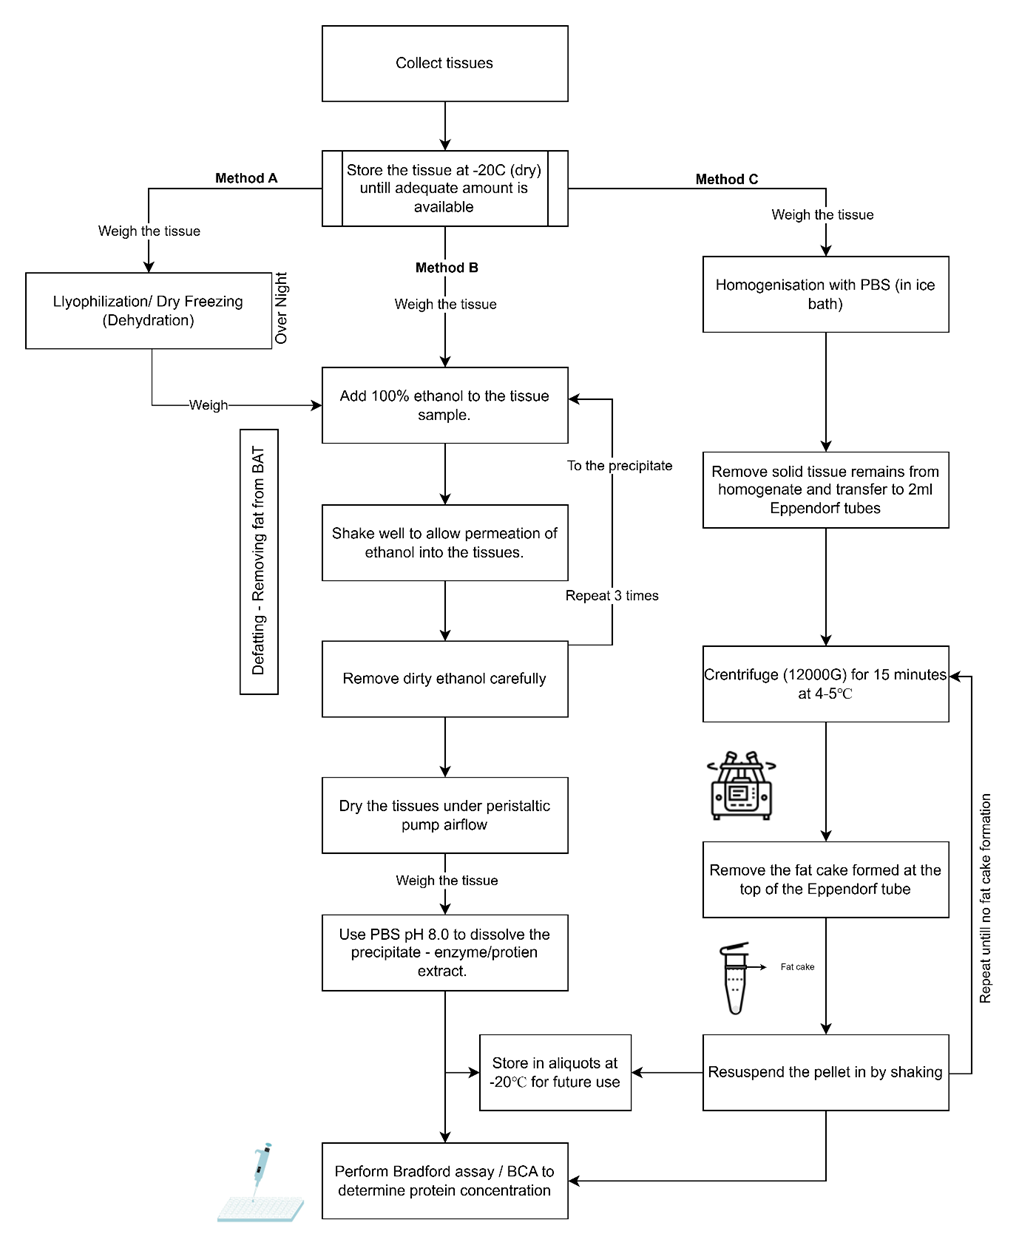
\includegraphics{images/clipboard-2471847056.png}

}

\caption{\label{fig-methodflow}Flow diagram of steps involved in
extracting SSAO from rat brown adipose tissue using Method A, Method B
and Method C}

\end{figure}%

\subsection{\texorpdfstring{\textbf{Protein
Quantification}}{Protein Quantification}}\label{sec-protein-quantification}

Bradford and BCA assays were performed to determine the concentration of
proteins in each extract. Bradford assay quantifies the protein
concentration by measuring the amino acid residues that binds to the
Coomassie Brilliant Blue G-250 dye.

Proteins present in the sample bind to the dye resulting in bright blue
appearance which can be measure at 595nm (Noble and Bailey 2009).
Alternatively, Bicinchoninic acid (BCA) assay was also performed due to
its high sensitivity and tolerance for interference. BCA measures the
protein concentration in two steps, first (biuret reaction) the peptide
bonds in the sample reduce the cupric ions in the reagent to cuprous
ions and then one cuprous ion chelates with 2 molecules of BCA to
produce an intense purple complex (Noble and Bailey 2009). This can be
measured at 562nm, as per the manufacturer's instructions.

Upon obtaining absorbances of undiluted stock samples that do not fit
inside the standard curve, the stock samples were diluted and read
again. The protein concentrations for the stock samples were calculated
by correcting the concentration of the diluted sample with the dilution
factor.

Known concentrations of Bovine Serum Albumin (BSA) is used to prepare a
standard curve which was used to interpolate absorbances obtained from
unknown samples (Noble \& Bailey, 2009). 10 mg of BSA was weighed and
dissolved in 10ml of deionised water to prepare a 1mg/ml stock BSA
standard. The 1mg/ml stock was used to prepare further dilutions as per
table 1.

\begin{longtable}[]{@{}
  >{\raggedright\arraybackslash}p{(\columnwidth - 4\tabcolsep) * \real{0.2500}}
  >{\raggedright\arraybackslash}p{(\columnwidth - 4\tabcolsep) * \real{0.3750}}
  >{\raggedright\arraybackslash}p{(\columnwidth - 4\tabcolsep) * \real{0.3750}}@{}}
\caption{BSA Standard dilution}\tabularnewline
\toprule\noalign{}
\begin{minipage}[b]{\linewidth}\raggedright
BSA Stock Volume
\end{minipage} & \begin{minipage}[b]{\linewidth}\raggedright
Deionised water volume (ml)
\end{minipage} & \begin{minipage}[b]{\linewidth}\raggedright
Final concentration (mg/ml)
\end{minipage} \\
\midrule\noalign{}
\endfirsthead
\toprule\noalign{}
\begin{minipage}[b]{\linewidth}\raggedright
BSA Stock Volume
\end{minipage} & \begin{minipage}[b]{\linewidth}\raggedright
Deionised water volume (ml)
\end{minipage} & \begin{minipage}[b]{\linewidth}\raggedright
Final concentration (mg/ml)
\end{minipage} \\
\midrule\noalign{}
\endhead
\bottomrule\noalign{}
\endlastfoot
0.8 & 0.2 & 0.8 \\
0.6 & 0.4 & 0.6 \\
0.4 & 0.6 & 0.4 \\
0.2 & 0.8 & 0.2 \\
\end{longtable}

\subsubsection{\texorpdfstring{\textbf{Bradford
assay}}{Bradford assay}}\label{bradford-assay}

10µl of each standard (2 replicates) and extracts (5 replicates) from
each method was pipetted into each well of a 96 well plate with 200µl of
Bradford reagent. Deionized water was used as blank for standards, and
PBS was used as the blank for samples. 200µl of Bradford reagent was
added to the wells containing the blanks. The plates were read using BMG
Labtech CLARIOstar plate reader at 595nm. The stock sample from all
methods were diluted 10-fold and the absorbance was corrected with the
dilution factor. The absorbance readings were transferred to excel and
then to GraphPad prism to plot standard curves and estimate unknown
protein concentrations from the linear standard curve equation. However,
for the purpose of displaying the results, same analysis are performed
using R.

\begin{Shaded}
\begin{Highlighting}[]
\FunctionTok{library}\NormalTok{(tidyverse)}
\CommentTok{\# Data: Standard Concentration and Absorbance values}
\NormalTok{bradford\_sc }\OtherTok{\textless{}{-}} \FunctionTok{tibble}\NormalTok{(}
  \AttributeTok{standard\_Concentration =} \FunctionTok{c}\NormalTok{(}\FloatTok{1.0}\NormalTok{, }\FloatTok{0.8}\NormalTok{, }\FloatTok{0.6}\NormalTok{, }\FloatTok{0.4}\NormalTok{, }\FloatTok{0.2}\NormalTok{, }\FloatTok{0.0}\NormalTok{),}
  \AttributeTok{absorbance\_1 =} \FunctionTok{c}\NormalTok{(}\FloatTok{0.682}\NormalTok{, }\FloatTok{0.592}\NormalTok{, }\FloatTok{0.499}\NormalTok{, }\FloatTok{0.334}\NormalTok{, }\FloatTok{0.138}\NormalTok{, }\DecValTok{0}\NormalTok{),}
  \AttributeTok{absorbance\_2 =} \FunctionTok{c}\NormalTok{(}\FloatTok{0.725}\NormalTok{, }\FloatTok{0.61}\NormalTok{, }\FloatTok{0.493}\NormalTok{, }\FloatTok{0.324}\NormalTok{, }\FloatTok{0.161}\NormalTok{, }\DecValTok{0}\NormalTok{)}
\NormalTok{)}

\CommentTok{\# Calculate the mean absorbance}
\NormalTok{bradford\_sc}\SpecialCharTok{$}\NormalTok{mean\_absorbance }\OtherTok{\textless{}{-}} \FunctionTok{rowMeans}\NormalTok{(bradford\_sc[, }\FunctionTok{c}\NormalTok{(}\StringTok{"absorbance\_1"}\NormalTok{, }\StringTok{"absorbance\_2"}\NormalTok{)])}

\CommentTok{\# Fit a linear model}
\NormalTok{brad\_model }\OtherTok{\textless{}{-}} \FunctionTok{lm}\NormalTok{(mean\_absorbance }\SpecialCharTok{\textasciitilde{}}\NormalTok{ standard\_Concentration, }\AttributeTok{data =}\NormalTok{ bradford\_sc)}

\CommentTok{\# Extract the equation and R{-}squared value}
\NormalTok{coefficients }\OtherTok{\textless{}{-}} \FunctionTok{coef}\NormalTok{(brad\_model)}
\NormalTok{intercept }\OtherTok{\textless{}{-}} \FunctionTok{round}\NormalTok{(coefficients[}\DecValTok{1}\NormalTok{], }\DecValTok{4}\NormalTok{)}
\NormalTok{slope }\OtherTok{\textless{}{-}} \FunctionTok{round}\NormalTok{(coefficients[}\DecValTok{2}\NormalTok{], }\DecValTok{4}\NormalTok{)}
\NormalTok{r\_squared }\OtherTok{\textless{}{-}} \FunctionTok{round}\NormalTok{(}\FunctionTok{summary}\NormalTok{(brad\_model)}\SpecialCharTok{$}\NormalTok{r.squared, }\DecValTok{4}\NormalTok{)}
\NormalTok{equation }\OtherTok{\textless{}{-}} \FunctionTok{paste0}\NormalTok{(}\StringTok{"y = "}\NormalTok{, slope, }\StringTok{"x + "}\NormalTok{, intercept)}

\CommentTok{\# Plotting the standard curve}
\FunctionTok{ggplot}\NormalTok{(bradford\_sc, }\FunctionTok{aes}\NormalTok{(}\AttributeTok{x =}\NormalTok{ standard\_Concentration, }\AttributeTok{y =}\NormalTok{ mean\_absorbance)) }\SpecialCharTok{+}
  \FunctionTok{geom\_point}\NormalTok{() }\SpecialCharTok{+}
  \FunctionTok{geom\_smooth}\NormalTok{(}\AttributeTok{method =} \StringTok{"lm"}\NormalTok{, }\AttributeTok{se =} \ConstantTok{FALSE}\NormalTok{, }\AttributeTok{color =} \StringTok{"blue"}\NormalTok{) }\SpecialCharTok{+}
  \FunctionTok{labs}\NormalTok{(}
    \AttributeTok{title =} \StringTok{"Bradford Assay {-} BSA Standard Curve"}\NormalTok{,}
    \AttributeTok{x =} \StringTok{"BSA Standard Concentration (mg/mL)"}\NormalTok{,}
    \AttributeTok{y =} \StringTok{"Mean Absorbance"}
\NormalTok{  ) }\SpecialCharTok{+}
  \FunctionTok{annotate}\NormalTok{(}\StringTok{"text"}\NormalTok{, }\AttributeTok{x =} \FloatTok{0.75}\NormalTok{, }\AttributeTok{y =} \FloatTok{0.1}\NormalTok{, }\AttributeTok{label =} \FunctionTok{paste}\NormalTok{(equation, }\StringTok{"}\SpecialCharTok{\textbackslash{}n}\StringTok{R² = "}\NormalTok{, r\_squared), }\AttributeTok{color =} \StringTok{"blue"}\NormalTok{) }\SpecialCharTok{+}
  \FunctionTok{theme\_classic}\NormalTok{()}
\end{Highlighting}
\end{Shaded}

\begin{figure}[H]

\centering{

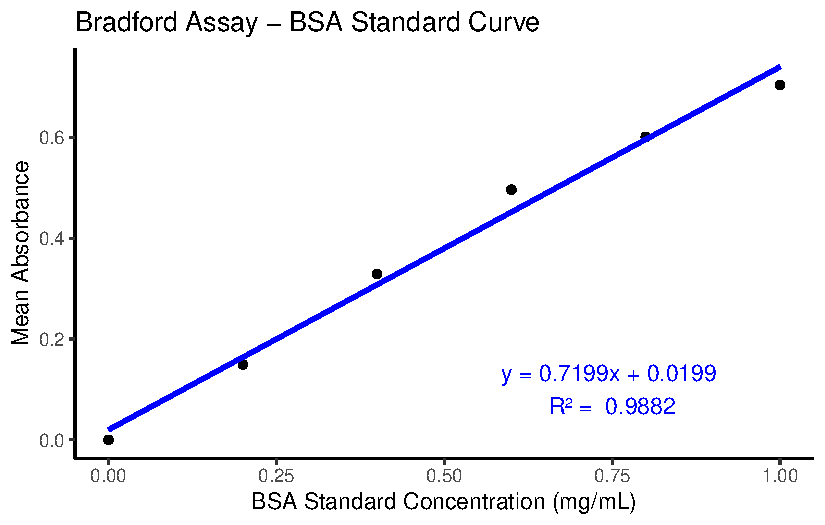
\includegraphics{materials_and_methods_files/figure-pdf/fig-brad-stdcurve-1.pdf}

}

\caption{\label{fig-brad-stdcurve}Standard Curve for BSA protein
concentration by Bradford assay. The absorbance was measured at 595nm
using BMG Labtech SPECTROstar plate reader.}

\end{figure}%

\subsubsection{\texorpdfstring{\textbf{BCA
assay}}{BCA assay}}\label{bca-assay}

BCA assay was performed to estimate the protein concentration in the
extracts obtained from Method A, Method B, and Method C. 25µl of
standard and sample were pipetted into each well of a clear flatbottom
96 well plate with 200µl of BCA reagent. The plates were incubated at
37℃ for 30 minutes and absorbance was measured at 562nm using the BMG
Labtech CLARIOstar plate reader. The stock sample from all methods were
diluted 10-fold and the absorbance was corrected with the dilution
factor.

\begin{Shaded}
\begin{Highlighting}[]
\FunctionTok{library}\NormalTok{(tidyverse)}
\CommentTok{\# Data: Standard Concentration and Absorbance values}
\NormalTok{bca\_sc }\OtherTok{\textless{}{-}} \FunctionTok{tibble}\NormalTok{(}
  \AttributeTok{standard\_Concentration =} \FunctionTok{c}\NormalTok{(}\FloatTok{1.0}\NormalTok{, }\FloatTok{0.8}\NormalTok{, }\FloatTok{0.6}\NormalTok{, }\FloatTok{0.4}\NormalTok{, }\FloatTok{0.2}\NormalTok{, }\FloatTok{0.0}\NormalTok{),}
  \AttributeTok{absorbance\_1 =} \FunctionTok{c}\NormalTok{(}\FloatTok{1.263}\NormalTok{, }\FloatTok{0.976}\NormalTok{, }\FloatTok{0.749}\NormalTok{, }\FloatTok{0.602}\NormalTok{, }\FloatTok{0.291}\NormalTok{, }\DecValTok{0}\NormalTok{),}
  \AttributeTok{absorbance\_2 =} \FunctionTok{c}\NormalTok{(}\FloatTok{1.162}\NormalTok{, }\FloatTok{0.943}\NormalTok{, }\FloatTok{0.663}\NormalTok{, }\FloatTok{0.498}\NormalTok{, }\FloatTok{0.266}\NormalTok{, }\DecValTok{0}\NormalTok{)}
\NormalTok{)}

\NormalTok{bca\_sc}\SpecialCharTok{$}\NormalTok{mean\_absorbance }\OtherTok{\textless{}{-}} \FunctionTok{rowMeans}\NormalTok{(bca\_sc[, }\FunctionTok{c}\NormalTok{(}\StringTok{"absorbance\_1"}\NormalTok{, }\StringTok{"absorbance\_2"}\NormalTok{)])}

\CommentTok{\# Fit a linear model}
\NormalTok{bca\_model }\OtherTok{\textless{}{-}} \FunctionTok{lm}\NormalTok{(mean\_absorbance }\SpecialCharTok{\textasciitilde{}}\NormalTok{ standard\_Concentration, }\AttributeTok{data =}\NormalTok{ bca\_sc)}

\CommentTok{\# Extract the equation and R{-}squared value}
\NormalTok{coefficients }\OtherTok{\textless{}{-}} \FunctionTok{coef}\NormalTok{(bca\_model)}
\NormalTok{intercept }\OtherTok{\textless{}{-}} \FunctionTok{round}\NormalTok{(coefficients[}\DecValTok{1}\NormalTok{], }\DecValTok{4}\NormalTok{)}
\NormalTok{slope }\OtherTok{\textless{}{-}} \FunctionTok{round}\NormalTok{(coefficients[}\DecValTok{2}\NormalTok{], }\DecValTok{4}\NormalTok{)}
\NormalTok{r\_squared }\OtherTok{\textless{}{-}} \FunctionTok{round}\NormalTok{(}\FunctionTok{summary}\NormalTok{(bca\_model)}\SpecialCharTok{$}\NormalTok{r.squared, }\DecValTok{4}\NormalTok{)}
\NormalTok{equation }\OtherTok{\textless{}{-}} \FunctionTok{paste0}\NormalTok{(}\StringTok{"y = "}\NormalTok{, slope, }\StringTok{"x + "}\NormalTok{, intercept)}

\CommentTok{\# Plotting the standard curve}
\FunctionTok{ggplot}\NormalTok{(bca\_sc, }\FunctionTok{aes}\NormalTok{(}\AttributeTok{x =}\NormalTok{ standard\_Concentration, }\AttributeTok{y =}\NormalTok{ mean\_absorbance)) }\SpecialCharTok{+}
  \FunctionTok{geom\_point}\NormalTok{() }\SpecialCharTok{+}
  \FunctionTok{geom\_smooth}\NormalTok{(}\AttributeTok{method =} \StringTok{"lm"}\NormalTok{, }\AttributeTok{se =} \ConstantTok{FALSE}\NormalTok{, }\AttributeTok{color =} \StringTok{"blue"}\NormalTok{) }\SpecialCharTok{+}
  \FunctionTok{labs}\NormalTok{(}
    \AttributeTok{title =} \StringTok{"BCA Assay {-} BSA Standard Curve"}\NormalTok{,}
    \AttributeTok{x =} \StringTok{"BSA Standard Concentration (mg/mL)"}\NormalTok{,}
    \AttributeTok{y =} \StringTok{"Mean Absorbance"}
\NormalTok{  ) }\SpecialCharTok{+}
  \FunctionTok{annotate}\NormalTok{(}\StringTok{"text"}\NormalTok{, }\AttributeTok{x =} \FloatTok{0.75}\NormalTok{, }\AttributeTok{y =} \FloatTok{0.1}\NormalTok{, }\AttributeTok{label =} \FunctionTok{paste}\NormalTok{(equation, }\StringTok{"}\SpecialCharTok{\textbackslash{}n}\StringTok{R² = "}\NormalTok{, r\_squared), }\AttributeTok{color =} \StringTok{"blue"}\NormalTok{) }\SpecialCharTok{+}
  \FunctionTok{theme\_classic}\NormalTok{()}
\end{Highlighting}
\end{Shaded}

\begin{figure}[H]

\centering{

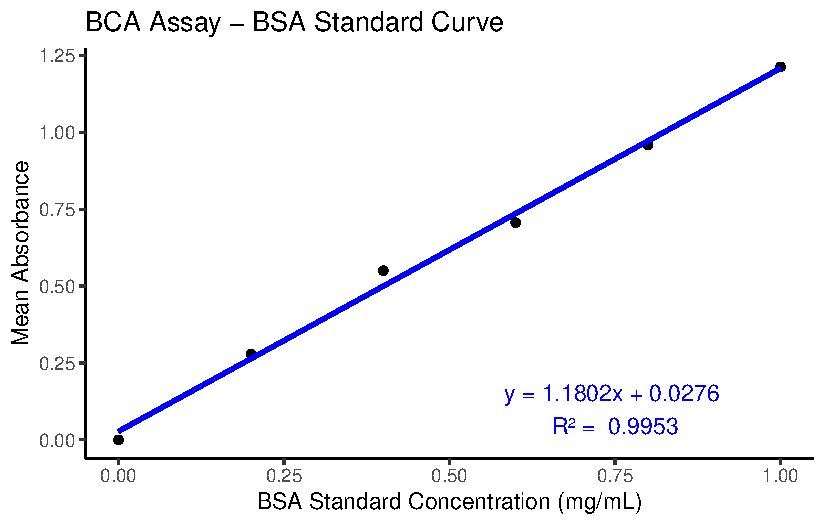
\includegraphics{materials_and_methods_files/figure-pdf/fig-bca-stdcurve-1.pdf}

}

\caption{\label{fig-bca-stdcurve}Standard Curve for BSA protein
concentration by BCA assay. The abosorbance was measured at 562nm using
BMG labtech SPECTROstar plate reader}

\end{figure}%

\subsection{\texorpdfstring{\textbf{Measurement of SSAO
activity.}}{Measurement of SSAO activity.}}\label{sec-measureSSAO}

SSAO activity is estimated by measuring the levels of hydrogen peroxide
(H\textsubscript{2}O\textsubscript{2}) produced in the samples. is
produced when benzylamine is catalysed by SSAO. Concentration of
H\textsubscript{2}O\textsubscript{2} produced in the reaction directly
corresponds to SSAO activity levels. Amplex\textsuperscript{®} red assay
is a highly specific fluorescence-based assay that can be used to
measure levels in the samples.

\subsubsection{\texorpdfstring{\textbf{Amplex}\textsuperscript{®}
\textbf{red monoamine oxidase assay}
\{\#sec-amplex®-red-monoamine-oxidase-assay\}}{Amplex® red monoamine oxidase assay \{\#sec-amplex®-red-monoamine-oxidase-assay\}}}\label{amplex-red-monoamine-oxidase-assay-sec-amplex-red-monoamine-oxidase-assay}

Amplex\textsuperscript{®} red is a colourless, non-fluorescent compound
that converts into resorufin in presence of
H\textsubscript{2}O\textsubscript{2} and Horseradish peroxidase.
Resorufin is a highly fluorescent product which has an absorption and
fluorescence emission maxima of approximately 571 nm and 585 nm,
respectively (Cai et al. 2022; Karakuzu et al. 2019).
Amplex\textsuperscript{®} red monoamine oxidase kit was obtained from
Thermo-Fisher scientific to measure the SSAO activity in the samples
prepared from various methods. The stock solutions for
Amplex\textsuperscript{®} red, HRP,
H\textsubscript{2}O\textsubscript{2}, Benzylamine, and Resorufin were
prepared as per manufacturer instructions

\begin{longtable}[]{@{}llll@{}}
\caption{Stock solution preparation for Amplex\textsuperscript{®} red
monoamine oxidase
assay}\label{tbl-amplex-red-stock-solution-prep}\tabularnewline
\toprule\noalign{}
Stock solution & Quantity/Volume & Diluent Volume & Stock Conc. \\
\midrule\noalign{}
\endfirsthead
\toprule\noalign{}
Stock solution & Quantity/Volume & Diluent Volume & Stock Conc. \\
\midrule\noalign{}
\endhead
\bottomrule\noalign{}
\endlastfoot
Amplex® red & 1Vial & 250µl DMSO & 20mM \\
5X reaction buffer & 5ml & 20ml dH2O & 1X buffer \\
HRP & 1Vial & 1ml 1X buffer & 200U/ml \\
Benzylamine & 1Vial & 1.2ml dH2O & 100mM \\
Resorufin & 1Vial & 1ml dH2O & 2mM \\
\end{longtable}

The stock solutions were used to prepare a reaction mixture containing
400µM Amplex\textsuperscript{®} red, 2U/ml HRP, and appropriate
substrate concentration. For example, 2000 µl of the reaction mixture
was prepared by combining 40µl Amplex\textsuperscript{®} red
stock(20mM), 20µl HRP stock(200U/ml), 1900µl sodium phosphate buffer (pH
7.4) (1X reaction buffer), and 40µl of benzylamine solution of the
desired concentration (Table~\ref{tbl-substrate-solution-prep}) . A
reaction mixture without substrate was prepared by replacing the
substrate with same volume of 1X reaction buffer. For measuring the
inhibitory activity of caffeine and simvastatin on SSAO, 10µL of each
inhibitor at 0 .1, 1, and 10mM concentration were added to the samples
and incubated for 15 minutes prior to adding the reaction mixture
containing the substrates triggering the enzyme reaction.

\begin{longtable}[]{@{}
  >{\raggedright\arraybackslash}p{(\columnwidth - 6\tabcolsep) * \real{0.2500}}
  >{\raggedright\arraybackslash}p{(\columnwidth - 6\tabcolsep) * \real{0.2500}}
  >{\raggedright\arraybackslash}p{(\columnwidth - 6\tabcolsep) * \real{0.2500}}
  >{\raggedright\arraybackslash}p{(\columnwidth - 6\tabcolsep) * \real{0.2500}}@{}}
\caption{Benzylamine substrate dilution for preparation of
Amplex\textsuperscript{®} red monoamine oxidase assay reaction
mixture.}\label{tbl-substrate-solution-prep}\tabularnewline
\toprule\noalign{}
\begin{minipage}[b]{\linewidth}\raggedright
Benzylamine Dilution
\end{minipage} & \begin{minipage}[b]{\linewidth}\raggedright
Stock volume
\end{minipage} & \begin{minipage}[b]{\linewidth}\raggedright
dH2O - Diluent Volume
\end{minipage} & \begin{minipage}[b]{\linewidth}\raggedright
Final concentration
\end{minipage} \\
\midrule\noalign{}
\endfirsthead
\toprule\noalign{}
\begin{minipage}[b]{\linewidth}\raggedright
Benzylamine Dilution
\end{minipage} & \begin{minipage}[b]{\linewidth}\raggedright
Stock volume
\end{minipage} & \begin{minipage}[b]{\linewidth}\raggedright
dH2O - Diluent Volume
\end{minipage} & \begin{minipage}[b]{\linewidth}\raggedright
Final concentration
\end{minipage} \\
\midrule\noalign{}
\endhead
\bottomrule\noalign{}
\endlastfoot
Dilution 1 & 20µl of 100mM Benz & 1980µl & 1 mM \\
Dilution 2 & 1000µl of Dilution 1 & 1000µl & 0.5 mM \\
Dilution 3 & 1000µl of Dilution 2 & 1000µl & 0.25 mM \\
Dilution 4 & 1000µl of Dilution 3 & 1000µl & 0.125 mM \\
Dilution 5 & 1000µl of Dilution 4 & 1000µl & 0.0625 mM \\
\end{longtable}

Known concentrations of resorufin were prepared to produce a standard
curve. This standard curve is used to measure the moles of resorufin
produced as a result of SSAO activity in the samples. 120µl of each
resorufin standard dilution was pipetted in duplicates in individual
wells of a 96 opaque flatbottom well plate for the standard curve. For
samples, 60µl of sample prepared from method A, method B, and method C
were pipetted in individual wells and 60µl of reaction mixture
containing 10mM benzylamine substrate was added to the wells containing
the sample. The plates were incubated at 37℃ for 30 minutes prior to
measuring the fluorescence using BMG Labtech CLARIOstar plus plate
reader.

For continuous measurement of SSAO activity, the plates containing SSAO
without the reaction mixture were incubated at 37℃, and the incubator
attached to BMG Labtech CLARIOstar plate reader was also set at 37℃
during the analysis. For inhibitor kinetics measurements, the inhibitors
at different concentrations were added to the sample and were incubated
at 37℃ for 15 minutes without the reaction mixture.

\begin{longtable}[]{@{}lll@{}}
\caption{Resorufin dilution preparation for Amplex\textsuperscript{®}
red monoamine oxidase assay standard
curve.}\label{tbl-resorufin-soln-prep}\tabularnewline
\toprule\noalign{}
Resorufin Stock & dH2O (ml) & Final Concentration (µM) \\
\midrule\noalign{}
\endfirsthead
\toprule\noalign{}
Resorufin Stock & dH2O (ml) & Final Concentration (µM) \\
\midrule\noalign{}
\endhead
\bottomrule\noalign{}
\endlastfoot
Stock 2mM -- 20µl & 1980 µl & 20 µM \\
Stock 20 µM -- 100 µl & 100 µl & 10 µM \\
Stock 20 µM -- 80 µl & 120 µl & 8 µM \\
Stock 20 µM -- 60 µl & 140 µl & 6 µM \\
Stock 20 µM -- 40 µl & 160 µl & 4 µM \\
Stock 20 µM -- 20 µl & 180 µl & 2 µM \\
\end{longtable}

\begin{Shaded}
\begin{Highlighting}[]
\FunctionTok{library}\NormalTok{(tidyverse)}
\CommentTok{\# Data: Standard Concentration and Absorbance values}
\NormalTok{reso\_sc }\OtherTok{\textless{}{-}} \FunctionTok{tibble}\NormalTok{(}
  \AttributeTok{standard\_Concentration =} \FunctionTok{c}\NormalTok{(}\FloatTok{1.0}\NormalTok{, }\FloatTok{0.8}\NormalTok{, }\FloatTok{0.6}\NormalTok{, }\FloatTok{0.4}\NormalTok{, }\FloatTok{0.2}\NormalTok{, }\FloatTok{0.0}\NormalTok{),}
  \AttributeTok{absorbance\_1 =} \FunctionTok{c}\NormalTok{(}\DecValTok{233718}\NormalTok{, }\DecValTok{173498}\NormalTok{, }\DecValTok{136768}\NormalTok{, }\DecValTok{90371}\NormalTok{, }\DecValTok{49091}\NormalTok{, }\DecValTok{0}\NormalTok{),}
  \AttributeTok{absorbance\_2 =} \FunctionTok{c}\NormalTok{(}\DecValTok{231342}\NormalTok{, }\DecValTok{178368}\NormalTok{, }\DecValTok{141037}\NormalTok{, }\DecValTok{91900}\NormalTok{, }\DecValTok{48934}\NormalTok{, }\DecValTok{0}\NormalTok{)}
\NormalTok{)}

\NormalTok{reso\_sc}\SpecialCharTok{$}\NormalTok{mean\_absorbance }\OtherTok{\textless{}{-}} \FunctionTok{rowMeans}\NormalTok{(reso\_sc[, }\FunctionTok{c}\NormalTok{(}\StringTok{"absorbance\_1"}\NormalTok{, }\StringTok{"absorbance\_2"}\NormalTok{)])}

\CommentTok{\# Fit a linear model}
\NormalTok{reso\_model }\OtherTok{\textless{}{-}} \FunctionTok{lm}\NormalTok{(mean\_absorbance }\SpecialCharTok{\textasciitilde{}}\NormalTok{ standard\_Concentration, }\AttributeTok{data =}\NormalTok{ reso\_sc)}

\CommentTok{\# Extract the equation and R{-}squared value}
\NormalTok{coefficients }\OtherTok{\textless{}{-}} \FunctionTok{coef}\NormalTok{(reso\_model)}
\NormalTok{intercept }\OtherTok{\textless{}{-}} \FunctionTok{round}\NormalTok{(coefficients[}\DecValTok{1}\NormalTok{], }\DecValTok{0}\NormalTok{)}
\NormalTok{slope }\OtherTok{\textless{}{-}} \FunctionTok{round}\NormalTok{(coefficients[}\DecValTok{2}\NormalTok{], }\DecValTok{0}\NormalTok{)}
\NormalTok{r\_squared }\OtherTok{\textless{}{-}} \FunctionTok{round}\NormalTok{(}\FunctionTok{summary}\NormalTok{(reso\_model)}\SpecialCharTok{$}\NormalTok{r.squared, }\DecValTok{4}\NormalTok{)}
\NormalTok{equation }\OtherTok{\textless{}{-}} \FunctionTok{paste0}\NormalTok{(}\StringTok{"y = "}\NormalTok{, slope, }\StringTok{"x + "}\NormalTok{, intercept)}

\CommentTok{\# Plotting the standard curve}
\FunctionTok{ggplot}\NormalTok{(reso\_sc, }\FunctionTok{aes}\NormalTok{(}\AttributeTok{x =}\NormalTok{ standard\_Concentration, }\AttributeTok{y =}\NormalTok{ mean\_absorbance)) }\SpecialCharTok{+}
  \FunctionTok{geom\_point}\NormalTok{() }\SpecialCharTok{+}
  \FunctionTok{geom\_smooth}\NormalTok{(}\AttributeTok{method =} \StringTok{"lm"}\NormalTok{, }\AttributeTok{se =} \ConstantTok{FALSE}\NormalTok{, }\AttributeTok{color =} \StringTok{"blue"}\NormalTok{) }\SpecialCharTok{+}
  \FunctionTok{labs}\NormalTok{(}
    \AttributeTok{title =} \StringTok{"Amplex Red Assay {-} Resorufin Standard Curve"}\NormalTok{,}
    \AttributeTok{x =} \StringTok{"Resorufin Standard Concentration (µM)"}\NormalTok{,}
    \AttributeTok{y =} \StringTok{"Corrected RFU"}
\NormalTok{  ) }\SpecialCharTok{+}
  \FunctionTok{annotate}\NormalTok{(}\StringTok{"text"}\NormalTok{, }\AttributeTok{x =} \FloatTok{0.75}\NormalTok{, }\AttributeTok{y =} \DecValTok{5000}\NormalTok{, }\AttributeTok{label =} \FunctionTok{paste}\NormalTok{(equation, }\StringTok{"}\SpecialCharTok{\textbackslash{}n}\StringTok{R² = "}\NormalTok{, r\_squared), }\AttributeTok{color =} \StringTok{"blue"}\NormalTok{) }\SpecialCharTok{+}
  \FunctionTok{theme\_classic}\NormalTok{()}
\end{Highlighting}
\end{Shaded}

\begin{figure}[H]

\centering{

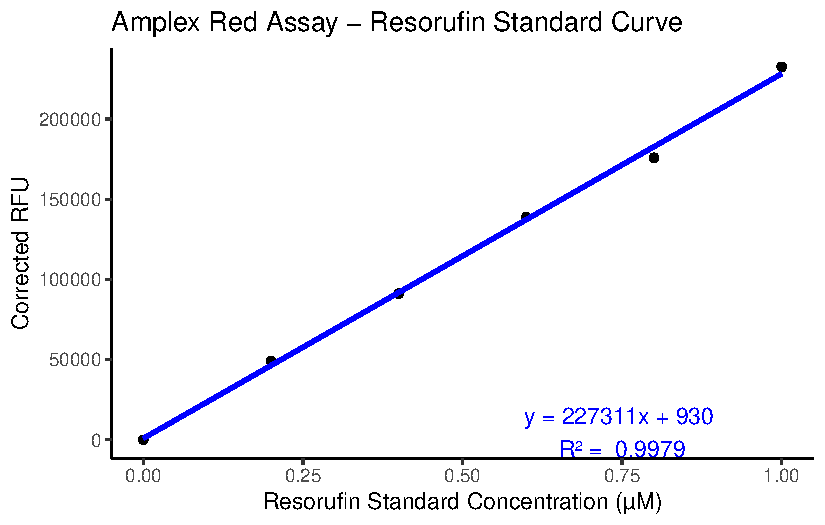
\includegraphics{materials_and_methods_files/figure-pdf/fig-reso-stdcurve-1.pdf}

}

\caption{\label{fig-reso-stdcurve}Standard Curve of Resorufin by Amplex®
red monoamine oxidase assay. RFU measured at 585mM emission maxima using
BMG Labtech CLARIOstar plus fluorescence plate reader.}

\end{figure}%

\textbf{\emph{Instrument settings for BMG Labtech CLARIOstar plus plate
reader.}}

A new protocol was created in the instrument for
Amplex\textsuperscript{®} red monoamine oxidase assay in plate mode and
endpoint mode. The protocols were set to measure fluorescence at an
excitation range of 540±20 and emission range of 590±20 as resorufin has
fluorescence emission maxima of approximately 585 nm. Gain settings and
focal length for the assays were set based on the wells containing 10 µM
resorufin as they are optimal for highest level of fluorescence.~ Gain
settings for plate mode were set at 90\% with a gain of 963 and a focal
length of 7.6 to yield consistent fluorescent across multiple readings.
These initial values were standardised from 10 µM resorufin fluorescence
readings. For a continuous kinetic assessment, plate mode with the
following settings were used. These settings were used to read the
fluorescence of each well every 30s for 10 minutes. The RFUs were used
to calculate the initial velocity of the enzymatic reaction.

\begin{longtable}[]{@{}ll@{}}
\caption{\emph{BMG Labtech CLARIOstar settings for plate mode
measurements of continuous kinetic
activity.}}\label{tbl-clairostar-instrument-setting}\tabularnewline
\toprule\noalign{}
Setting & Value \\
\midrule\noalign{}
\endfirsthead
\toprule\noalign{}
Setting & Value \\
\midrule\noalign{}
\endhead
\bottomrule\noalign{}
\endlastfoot
Optic & Top optic \\
Settling time & 0.5 \\
Measurement Start time & 0.0s \\
Number of intervals & 20 \\
Number of flashes & 20 \\
Interval time & 30s \\
\end{longtable}

\subsection{\texorpdfstring{\textbf{Statistical and data
analysis:}}{Statistical and data analysis:}}\label{statistical-and-data-analysis}

For the purposes of creating this Quarto book, data analysis was
performed using R. The results produced from the R code presented in
this manuscript were verified to match the results obtained from graphad
analysis.

All the data obtained from were recorded and formatted in Microsoft
excel. Further analysis such as generating a standard curve,
interpolating, and extrapolating values from standard curve for unknown
samples, and regression analysis was performed in GraphPad prism 10.
Slopes and intercepts represented in all graphs were calculated using
linear regression. Km, Ki, and Vmax values were calculated using
nonlinear regression using preset functions such as Michaelis Menten
equation and competitive inhibition in GraphPad prism. No parametric or
non-parametric analysis was performed in this project, as the number of
experiments does not meet the minimum sample size required for such
statistical analysis.

\bookmarksetup{startatroot}

\chapter{Results}\label{results}

The extracts obtained from each method were quantified using Bradford
and BCA assays. These samples were diluted 10-fold to fit the
absorbances obtained into the standard curve. The protein concentrations
of the dilutes samples were then calculated using the standard curve.
These results were corrected with the dilution factor to calculate the
estimated protein concentration of undiluted samples. The results are
tabulated and presented as mean Table~\ref{tbl-proteinestimate} and
compared in Figure~\ref{fig-proteinesti}. Amplex\textsuperscript{®} red
monoamine oxidase assay was used to determine the SSAO activity in the
samples from each method after treating the sample with the
Amplex\textsuperscript{®} red reaction mixture with 10mM benzylamine as
substrate and incubating at 37 ℃ for 30 minutes before measuring the
fluorescence. The results of SSAO activity from each sample is presented
in Table~\ref{tbl-ssaoactivity} and Figure~\ref{fig-ssaoactivity} .

\section{Method A}\label{method-a}

The tissues collected for a period of 4 days were weighed and freeze
dried using a freeze dryer to dehydrate the tissue. 11.1g of tissue were
freeze dried resulting in a loss of 71.1\% of weight(water) and 3.1g of
dehydrated tissue was obtained. Defatting of the dehydrated tissue
caused a further loss of 1g of fat weight, resulting in 2.1g of tissue.
Bradford assay and BCA assay were performed to estimate the protein
concentration in the extract obtained from this method A. Only one
independent experiment was performed using Method A (refer to 4.2.1) due
to unavailability of the freeze dryer during the project. The estimated
protein concentration of the extract obtained from method A is 4.2 mg/ml
(estimated by Bradford assay) and 4.5 mg/ml (estimated by the BCA
assay). The SSAO activity was measured with 10mM Benzylamine as
substrate and was found to be 2.02 µmol
H\textsubscript{2}O\textsubscript{2} /mg protein.

\section{Method B}\label{method-b}

Three independent experiments were performed by method B
Section~\ref{sec-method-b} for extracting SSAO from rat BAT. Frozen
tissues collected over 4 days were used for each experiment. Tissue
weights are presented in Table~\ref{tbl-defat} and the percentage of fat
lost was calculated from the dried tissue weight after treatment with
100\%EtOH. Bradford and BCA assays were performed to estimate the
protein concentrations in each extract and the results are presented and
compared as mean in Table~\ref{tbl-proteinestimate} and
Figure~\ref{fig-proteinesti} . The average amount of estimated protein
is 6.07 and 6.27 mg/ml by Bradford and BCA assays respectively. The
average SSAO activity was measured with 10mM Benzylamine was found to be
1.64 µmol H\textsubscript{2}O\textsubscript{2} /mg protein
Table~\ref{tbl-ssaoactivity} .

\begin{Shaded}
\begin{Highlighting}[]
\FunctionTok{library}\NormalTok{(tidyverse)}
\FunctionTok{library}\NormalTok{(knitr)}
\FunctionTok{library}\NormalTok{(patchwork)}
\NormalTok{defat\_results}\OtherTok{\textless{}{-}} \FunctionTok{tibble}\NormalTok{(}
  \AttributeTok{Experiment\_ID =} \FunctionTok{c}\NormalTok{(}\StringTok{"Experiment 1"}\NormalTok{, }\StringTok{"Experiment 2"}\NormalTok{, }\StringTok{"Experiment 3"}\NormalTok{),}
  \AttributeTok{Frozen\_weight\_g =}\FunctionTok{as.numeric}\NormalTok{(}\FunctionTok{c}\NormalTok{(}\FloatTok{10.81}\NormalTok{, }\FloatTok{9.64}\NormalTok{, }\FloatTok{10.25}\NormalTok{)),}
  \AttributeTok{Defatted\_dried\_weight\_g =} \FunctionTok{as.numeric}\NormalTok{(}\FunctionTok{c}\NormalTok{(}\FloatTok{4.62}\NormalTok{, }\FloatTok{5.91}\NormalTok{, }\FloatTok{7.31}\NormalTok{)),}
\NormalTok{) }\SpecialCharTok{|\textgreater{}} 
  \FunctionTok{mutate}\NormalTok{(}
    \AttributeTok{percentage\_fat\_lost =} \DecValTok{100}\SpecialCharTok{*}\NormalTok{(Frozen\_weight\_g }\SpecialCharTok{{-}}\NormalTok{ Defatted\_dried\_weight\_g)}\SpecialCharTok{/}\NormalTok{Frozen\_weight\_g}
\NormalTok{    )}
\FunctionTok{kable}\NormalTok{(defat\_results)}
\end{Highlighting}
\end{Shaded}

\begin{longtable}[]{@{}
  >{\raggedright\arraybackslash}p{(\columnwidth - 6\tabcolsep) * \real{0.1892}}
  >{\raggedleft\arraybackslash}p{(\columnwidth - 6\tabcolsep) * \real{0.2162}}
  >{\raggedleft\arraybackslash}p{(\columnwidth - 6\tabcolsep) * \real{0.3243}}
  >{\raggedleft\arraybackslash}p{(\columnwidth - 6\tabcolsep) * \real{0.2703}}@{}}

\toprule\noalign{}
\begin{minipage}[b]{\linewidth}\raggedright
Experiment\_ID
\end{minipage} & \begin{minipage}[b]{\linewidth}\raggedleft
Frozen\_weight\_g
\end{minipage} & \begin{minipage}[b]{\linewidth}\raggedleft
Defatted\_dried\_weight\_g
\end{minipage} & \begin{minipage}[b]{\linewidth}\raggedleft
percentage\_fat\_lost
\end{minipage} \\
\midrule\noalign{}
\endhead
\bottomrule\noalign{}
\endlastfoot
Experiment 1 & 10.81 & 4.62 & 57.26179 \\
Experiment 2 & 9.64 & 5.91 & 38.69295 \\
Experiment 3 & 10.25 & 7.31 & 28.68293 \\

\caption{\label{tbl-defat}Weights of rat BAT used in method B for
protein extraction.}

\tabularnewline

\end{longtable}

\section{\texorpdfstring{\textbf{Method C}}{Method C}}\label{method-c}

Three independent experiments were performed by Method C
Section~\ref{sec-method-c} . The tissues were weighed before cutting
into tiny pieces for homogenisation. Since there was no ideal way to
measure the amount of fat removed by centrifugation, percentage of fat
lost was not calculated for extracts obtained from method C. The average
estimated protein concentration for extracts obtained by method C is
5.27 and 5.43 mg/ml by Bradford and BCA assays respectively. The average
SSAO activity from samples obtained by method C was 0.02 µmol
H\textsubscript{2}O\textsubscript{2} /mg protein.

\begin{Shaded}
\begin{Highlighting}[]
\FunctionTok{library}\NormalTok{(tidyverse)}
\FunctionTok{library}\NormalTok{(knitr)}
\NormalTok{bradford\_BCA}\OtherTok{\textless{}{-}} \FunctionTok{tibble}\NormalTok{(}
  \AttributeTok{Experiment\_ID =} \FunctionTok{c}\NormalTok{(}\StringTok{"Experiment 1"}\NormalTok{, }\StringTok{"Experiment 2"}\NormalTok{, }\StringTok{"Experiment 3"}\NormalTok{, }
                    \StringTok{"Experiment 1"}\NormalTok{, }\StringTok{"Experiment 2"}\NormalTok{, }\StringTok{"Experiment 3"}\NormalTok{),}
  \AttributeTok{Method\_A =} \FunctionTok{as.numeric}\NormalTok{(}\FunctionTok{c}\NormalTok{(}\FloatTok{4.2}\NormalTok{, }\ConstantTok{NA}\NormalTok{, }\ConstantTok{NA}\NormalTok{, }\FloatTok{4.5}\NormalTok{, }\ConstantTok{NA}\NormalTok{, }\ConstantTok{NA}\NormalTok{)),}
  \AttributeTok{Method\_B =} \FunctionTok{c}\NormalTok{(}\FloatTok{6.4}\NormalTok{, }\FloatTok{5.8}\NormalTok{, }\FloatTok{6.0}\NormalTok{, }\FloatTok{6.5}\NormalTok{, }\FloatTok{6.1}\NormalTok{, }\FloatTok{6.2}\NormalTok{),}
  \AttributeTok{Method\_C =} \FunctionTok{c}\NormalTok{(}\FloatTok{5.1}\NormalTok{, }\FloatTok{4.9}\NormalTok{, }\FloatTok{5.8}\NormalTok{, }\FloatTok{5.4}\NormalTok{, }\DecValTok{5}\NormalTok{, }\FloatTok{5.9}\NormalTok{),}
  \AttributeTok{Assay =} \FunctionTok{c}\NormalTok{(}\StringTok{"Bradford"}\NormalTok{, }\StringTok{"Bradford"}\NormalTok{, }\StringTok{"Bradford"}\NormalTok{, }\StringTok{"BCA"}\NormalTok{, }\StringTok{"BCA"}\NormalTok{, }\StringTok{"BCA"}\NormalTok{)}
\NormalTok{)}
\FunctionTok{kable}\NormalTok{(bradford\_BCA)}
\end{Highlighting}
\end{Shaded}

\begin{longtable}[]{@{}lrrrl@{}}

\toprule\noalign{}
Experiment\_ID & Method\_A & Method\_B & Method\_C & Assay \\
\midrule\noalign{}
\endhead
\bottomrule\noalign{}
\endlastfoot
Experiment 1 & 4.2 & 6.4 & 5.1 & Bradford \\
Experiment 2 & NA & 5.8 & 4.9 & Bradford \\
Experiment 3 & NA & 6.0 & 5.8 & Bradford \\
Experiment 1 & 4.5 & 6.5 & 5.4 & BCA \\
Experiment 2 & NA & 6.1 & 5.0 & BCA \\
Experiment 3 & NA & 6.2 & 5.9 & BCA \\

\caption{\label{tbl-proteinestimate}Estimated protein concentration
(mg/ml) by Bradford and BCA assay for samples obtained by Method A (One
independent experiment), and Method B and Method C (3 independent
experiments)}

\tabularnewline

\end{longtable}

\begin{Shaded}
\begin{Highlighting}[]
\NormalTok{mean\_data }\OtherTok{\textless{}{-}}
\NormalTok{  bradford\_BCA }\SpecialCharTok{|\textgreater{}} 
  \FunctionTok{group\_by}\NormalTok{(Assay) }\SpecialCharTok{|\textgreater{}} 
  \FunctionTok{summarise}\NormalTok{(}\FunctionTok{across}\NormalTok{(}\FunctionTok{starts\_with}\NormalTok{(}\StringTok{"method"}\NormalTok{), mean, }\AttributeTok{na.rm =} \ConstantTok{TRUE}\NormalTok{)) }\SpecialCharTok{|\textgreater{}} 
  \FunctionTok{pivot\_longer}\NormalTok{(}\AttributeTok{cols =} \FunctionTok{starts\_with}\NormalTok{(}\StringTok{"method"}\NormalTok{),}
               \AttributeTok{names\_to =} \StringTok{"Method"}\NormalTok{,}
               \AttributeTok{values\_to =} \StringTok{"Mean"}\NormalTok{)}

\FunctionTok{ggplot}\NormalTok{(mean\_data, }\FunctionTok{aes}\NormalTok{(}\AttributeTok{x =}\NormalTok{ Method, }\AttributeTok{y =}\NormalTok{ Mean, }\AttributeTok{fill =}\NormalTok{ Assay)) }\SpecialCharTok{+}
  \FunctionTok{geom\_bar}\NormalTok{(}\AttributeTok{stat =} \StringTok{"identity"}\NormalTok{, }\AttributeTok{position =} \FunctionTok{position\_dodge}\NormalTok{(}\AttributeTok{width =} \FloatTok{0.9}\NormalTok{))}\SpecialCharTok{+} 
  \FunctionTok{scale\_y\_continuous}\NormalTok{(}\AttributeTok{limits =} \FunctionTok{c}\NormalTok{(}\DecValTok{0}\NormalTok{, }\DecValTok{7}\NormalTok{))}\SpecialCharTok{+}
  \FunctionTok{labs}\NormalTok{(}
    \AttributeTok{title =} \StringTok{"Protein estimates by Bradford assay (mg/ml)"}\NormalTok{, }
    \AttributeTok{x =} \ConstantTok{NULL}\NormalTok{, }
    \AttributeTok{y =} \StringTok{"Average protein}\SpecialCharTok{\textbackslash{}n}\StringTok{concentration estimate (mg/ml)"}
\NormalTok{  ) }\SpecialCharTok{+}
  \FunctionTok{theme\_minimal}\NormalTok{() }\SpecialCharTok{+}
  \FunctionTok{scale\_fill\_manual}\NormalTok{(}\AttributeTok{values =} \FunctionTok{c}\NormalTok{(}\StringTok{"Bradford"} \OtherTok{=} \StringTok{"black"}\NormalTok{, }\StringTok{"BCA"} \OtherTok{=} \StringTok{"grey"}\NormalTok{)) }\SpecialCharTok{+}
  \FunctionTok{theme}\NormalTok{(}
    \AttributeTok{plot.title =} \FunctionTok{element\_text}\NormalTok{(}\AttributeTok{size =} \DecValTok{14}\NormalTok{, }\AttributeTok{hjust =} \FloatTok{0.5}\NormalTok{),}
    \AttributeTok{axis.title.y =} \FunctionTok{element\_text}\NormalTok{(}\AttributeTok{size =} \DecValTok{12}\NormalTok{, }\AttributeTok{margin =} \FunctionTok{margin}\NormalTok{(}\AttributeTok{t =} \DecValTok{0}\NormalTok{, }\AttributeTok{r =} \DecValTok{15}\NormalTok{, }\AttributeTok{b =} \DecValTok{0}\NormalTok{, }\AttributeTok{l =} \DecValTok{0}\NormalTok{)),}
    \AttributeTok{axis.text.x =} \FunctionTok{element\_text}\NormalTok{(}\AttributeTok{size =} \DecValTok{10}\NormalTok{),}
    \AttributeTok{axis.text.y =} \FunctionTok{element\_text}\NormalTok{(}\AttributeTok{size =} \DecValTok{10}\NormalTok{),}
    \AttributeTok{legend.title =} \FunctionTok{element\_text}\NormalTok{(}\AttributeTok{size =} \DecValTok{10}\NormalTok{),}
    \AttributeTok{legend.text =} \FunctionTok{element\_text}\NormalTok{(}\AttributeTok{size =} \DecValTok{9}\NormalTok{),}
    \AttributeTok{legend.position =} \StringTok{"right"}\NormalTok{,}
    \AttributeTok{plot.margin =} \FunctionTok{margin}\NormalTok{(}\DecValTok{10}\NormalTok{, }\DecValTok{10}\NormalTok{, }\DecValTok{10}\NormalTok{, }\DecValTok{10}\NormalTok{)}
\NormalTok{  ) }\SpecialCharTok{+}
  \FunctionTok{geom\_text}\NormalTok{(}
    \FunctionTok{aes}\NormalTok{(}\AttributeTok{label =} \FunctionTok{round}\NormalTok{(Mean, }\DecValTok{2}\NormalTok{)),}
    \AttributeTok{vjust =} \SpecialCharTok{{-}}\FloatTok{0.5}\NormalTok{,}
    \AttributeTok{position =} \FunctionTok{position\_dodge}\NormalTok{(}\AttributeTok{width =} \FloatTok{0.9}\NormalTok{),}
    \AttributeTok{size =} \DecValTok{3}
\NormalTok{  )}\SpecialCharTok{+} \FunctionTok{theme\_classic}\NormalTok{()}
\end{Highlighting}
\end{Shaded}

\begin{figure}[H]

\centering{

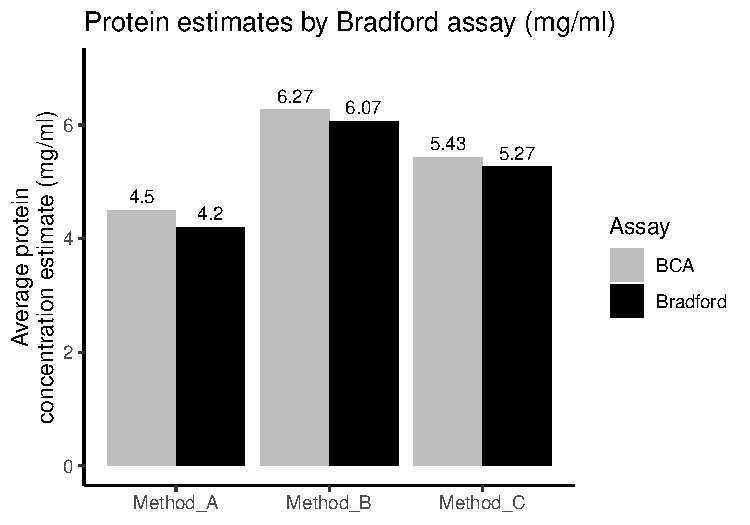
\includegraphics{results_files/figure-pdf/fig-proteinesti-1.pdf}

}

\caption{\label{fig-proteinesti}Comparision of average protein
concentration estimate in extracts obtained from Method\_A, Method\_B,
and Method\_C by BCA and Bradford assays.}

\end{figure}%

\begin{Shaded}
\begin{Highlighting}[]
\FunctionTok{library}\NormalTok{(tidyverse)}
\FunctionTok{library}\NormalTok{(knitr)}
\NormalTok{ssao\_activity}\OtherTok{\textless{}{-}} \FunctionTok{tibble}\NormalTok{(}
  \AttributeTok{Experiment\_ID =} \FunctionTok{c}\NormalTok{(}\StringTok{"Experiment 1"}\NormalTok{, }\StringTok{"Experiment 2"}\NormalTok{, }\StringTok{"Experiment 3"}\NormalTok{),}
  \AttributeTok{Method\_A =} \FunctionTok{as.numeric}\NormalTok{(}\FunctionTok{c}\NormalTok{(}\FloatTok{2.018182}\NormalTok{, }\ConstantTok{NA}\NormalTok{, }\ConstantTok{NA}\NormalTok{)),}
  \AttributeTok{Method\_B =} \FunctionTok{c}\NormalTok{(}\FloatTok{1.553474}\NormalTok{, }\FloatTok{1.72336}\NormalTok{, }\FloatTok{1.649069}\NormalTok{),}
  \AttributeTok{Method\_C =} \FunctionTok{c}\NormalTok{(}\FloatTok{0.024903}\NormalTok{, }\FloatTok{0.013653}\NormalTok{, }\FloatTok{0.011098}\NormalTok{),}
\NormalTok{)}

\NormalTok{means\_row }\OtherTok{\textless{}{-}} \FunctionTok{tibble}\NormalTok{(}
  \AttributeTok{Experiment\_ID =} \StringTok{"Mean"}\NormalTok{,}
  \AttributeTok{Method\_A =} \FunctionTok{mean}\NormalTok{(ssao\_activity}\SpecialCharTok{$}\NormalTok{Method\_A, }\AttributeTok{na.rm =} \ConstantTok{TRUE}\NormalTok{),}
  \AttributeTok{Method\_B =} \FunctionTok{mean}\NormalTok{(ssao\_activity}\SpecialCharTok{$}\NormalTok{Method\_B, }\AttributeTok{na.rm =} \ConstantTok{TRUE}\NormalTok{),}
  \AttributeTok{Method\_C =} \FunctionTok{mean}\NormalTok{(ssao\_activity}\SpecialCharTok{$}\NormalTok{Method\_C, }\AttributeTok{na.rm =} \ConstantTok{TRUE}\NormalTok{)}
\NormalTok{)}

\NormalTok{ssao\_activity\_with\_means }\OtherTok{\textless{}{-}} \FunctionTok{bind\_rows}\NormalTok{(ssao\_activity, means\_row)}
\FunctionTok{kable}\NormalTok{(ssao\_activity\_with\_means)}
\end{Highlighting}
\end{Shaded}

\begin{longtable}[]{@{}lrrr@{}}

\toprule\noalign{}
Experiment\_ID & Method\_A & Method\_B & Method\_C \\
\midrule\noalign{}
\endhead
\bottomrule\noalign{}
\endlastfoot
Experiment 1 & 2.018182 & 1.553474 & 0.0249030 \\
Experiment 2 & NA & 1.723360 & 0.0136530 \\
Experiment 3 & NA & 1.649069 & 0.0110980 \\
Mean & 2.018182 & 1.641968 & 0.0165513 \\

\caption{\label{tbl-ssaoactivity}SSAO activity corrected to protein
concentration from respective BCA results for Method A (One independent
experiment), and Method B and Method C (3 independent experiments}

\tabularnewline

\end{longtable}

\begin{Shaded}
\begin{Highlighting}[]
\NormalTok{means\_row }\SpecialCharTok{|\textgreater{}} \FunctionTok{pivot\_longer}\NormalTok{(}\AttributeTok{cols =} \FunctionTok{starts\_with}\NormalTok{(}\StringTok{"Method"}\NormalTok{),}
                          \AttributeTok{names\_to =} \StringTok{"Method"}\NormalTok{,}
                          \AttributeTok{values\_to =} \StringTok{"Mean"}\NormalTok{) }\SpecialCharTok{|\textgreater{}} 
  \FunctionTok{ggplot}\NormalTok{(}\FunctionTok{aes}\NormalTok{(}\AttributeTok{x =}\NormalTok{ Method, }\AttributeTok{y =}\NormalTok{ Mean))}\SpecialCharTok{+}
  \FunctionTok{geom\_bar}\NormalTok{(}\AttributeTok{stat =} \StringTok{"identity"}\NormalTok{, }\AttributeTok{fill =} \StringTok{"black"}\NormalTok{, }\AttributeTok{width =} \FloatTok{0.5}
\NormalTok{           )}\SpecialCharTok{+} \FunctionTok{theme\_classic}\NormalTok{()}\SpecialCharTok{+}
  \FunctionTok{coord\_cartesian}\NormalTok{(}\AttributeTok{ylim =} \FunctionTok{c}\NormalTok{(}\DecValTok{0}\NormalTok{, }\FloatTok{2.5}\NormalTok{))}\SpecialCharTok{+}
  \FunctionTok{geom\_text}\NormalTok{(}\FunctionTok{aes}\NormalTok{(}\AttributeTok{label =} \FunctionTok{round}\NormalTok{(Mean, }\DecValTok{2}\NormalTok{)),}
    \AttributeTok{vjust =} \SpecialCharTok{{-}}\FloatTok{0.5}\NormalTok{,}
    \AttributeTok{position =} \FunctionTok{position\_dodge}\NormalTok{(}\AttributeTok{width =} \FloatTok{0.9}\NormalTok{),}
    \AttributeTok{size =} \DecValTok{3}\NormalTok{)}\SpecialCharTok{+}
  \FunctionTok{labs}\NormalTok{(}\AttributeTok{title =} \StringTok{"SSAO activity"}\NormalTok{,}
       \AttributeTok{x =} \ConstantTok{NULL}\NormalTok{,}
       \AttributeTok{y =} \StringTok{"SSAO activity}\SpecialCharTok{\textbackslash{}n}\StringTok{ µmol H2O2 /mg protein "}\NormalTok{)}
\end{Highlighting}
\end{Shaded}

\begin{figure}[H]

\centering{

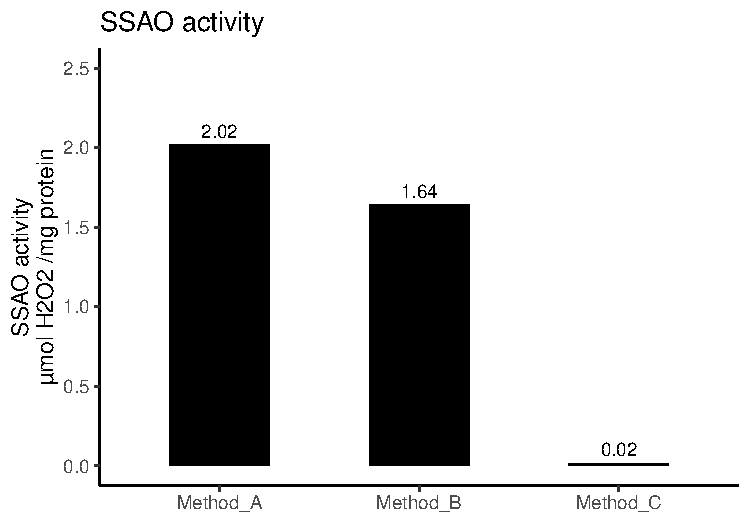
\includegraphics{results_files/figure-pdf/fig-ssaoactivity-1.pdf}

}

\caption{\label{fig-ssaoactivity}Comparison SSAO activity corrected to
protein concentration from respective BCA results for Method A (One
independent experiment), and Method B and Method C (3 independent
experiments).}

\end{figure}%

\section{Enzyme Kinetics}\label{enzyme-kinetics}

The extract obtained from Experiment 1 of method B is used to measure
the kinetic activity of SSAO by Amplex\textsuperscript{®} red monoamine
oxidase assay. The SSAO activity was measured as described in
Section~\ref{sec-measureSSAO} . For measuring the continuous kinetic
activity of SSAO, the instrument was setup in plate mode which measured
the fluorescence every 30 seconds for 10 minutes. The fluorescence
measurements resulting from the reaction mixture were used as blanks and
all the values were corrected accordingly. The gain settings and focal
length were maintained constant to obtain consistent readings.

Resorufin at different concentrations was used to establish a standard
curve to determine the slope and offset using a linear regression curve.
The fluorescence readings were exported into excel and formatted to
ensure a consistent data format for processing. The mean of the
replicate readings was converted into equivalent
H\textsubscript{2}O\textsubscript{2} concentrations using the resorufin
standard curve equation. These values were plotted against time in
minutes to calculate the change in H\textsubscript{2}O\textsubscript{2}
concentration over time using linear regression.

Individual curves were plotted for values obtained from each benzylamine
concentration.

\begin{equation}\phantomsection\label{eq-mm}{
{V0} = \frac{Vmax * [S]}{Km + [S]}
}\end{equation}

\begin{Shaded}
\begin{Highlighting}[]
\FunctionTok{library}\NormalTok{(broom)}
\FunctionTok{library}\NormalTok{(ggpubr)}

\CommentTok{\# Importing the data from a csv file}
\NormalTok{kinetic\_data }\OtherTok{\textless{}{-}} \FunctionTok{read\_csv}\NormalTok{(}\StringTok{"E:/LearningR/rforlearn/GIT/academic\_works/kinetic\_data.csv"}\NormalTok{)}

\CommentTok{\# Pivoting the data to fit the visualisation needs}

\NormalTok{kinetic\_data\_pivot }\OtherTok{\textless{}{-}}\NormalTok{ kinetic\_data }\SpecialCharTok{|\textgreater{}} 
  \FunctionTok{pivot\_longer}\NormalTok{(}
    \AttributeTok{cols =} \SpecialCharTok{!}\NormalTok{(}\FunctionTok{starts\_with}\NormalTok{(}\StringTok{"Time"}\NormalTok{)),}
    \AttributeTok{names\_to =} \FunctionTok{c}\NormalTok{(}\StringTok{"test\_group"}\NormalTok{, }\StringTok{"inhibitor\_concn"}\NormalTok{, }\StringTok{"substrate\_concn"}\NormalTok{),}
    \AttributeTok{names\_sep =} \StringTok{"\_"}\NormalTok{,}
    \AttributeTok{values\_to =} \StringTok{"ssao\_activity"}
\NormalTok{  ) }\SpecialCharTok{|\textgreater{}} \FunctionTok{mutate}\NormalTok{(}\AttributeTok{inhibitor\_concn =} \FunctionTok{parse\_number}\NormalTok{(inhibitor\_concn),}
              \AttributeTok{substrate\_concn =} \FunctionTok{parse\_number}\NormalTok{(substrate\_concn))}

\CommentTok{\# Isolating the ssao activity for control group for plot}

\NormalTok{kinetic\_data\_pivot }\SpecialCharTok{|\textgreater{}} 
  \FunctionTok{group\_by}\NormalTok{(test\_group) }\SpecialCharTok{|\textgreater{}} 
  \FunctionTok{filter}\NormalTok{(test\_group }\SpecialCharTok{==} \StringTok{"Control"}\NormalTok{) }\SpecialCharTok{|\textgreater{}} \FunctionTok{mutate}\NormalTok{(}\AttributeTok{substrate\_concn =} \FunctionTok{factor}\NormalTok{(substrate\_concn)) }\SpecialCharTok{|\textgreater{}} 
  \FunctionTok{ggplot}\NormalTok{(}\FunctionTok{aes}\NormalTok{(}\AttributeTok{x =} \StringTok{\textasciigrave{}}\AttributeTok{Time (min)}\StringTok{\textasciigrave{}}\NormalTok{, }
             \AttributeTok{y =}\NormalTok{ ssao\_activity, }
             \AttributeTok{color =}\NormalTok{ substrate\_concn, }
             \AttributeTok{group =}\NormalTok{ substrate\_concn))}\SpecialCharTok{+} 
  \FunctionTok{geom\_point}\NormalTok{() }\SpecialCharTok{+} 
  \FunctionTok{geom\_smooth}\NormalTok{(}
    \AttributeTok{method =} \StringTok{"lm"}\NormalTok{,}
    \AttributeTok{formula =}\NormalTok{ y }\SpecialCharTok{\textasciitilde{}}\NormalTok{ x,}
    \AttributeTok{se =} \ConstantTok{FALSE}\NormalTok{,}
\NormalTok{    )}\SpecialCharTok{+}
  \FunctionTok{labs}\NormalTok{(}
    \AttributeTok{title =} \StringTok{"SSAO kinetics {-} Control"}\NormalTok{,}
    \AttributeTok{y =} \StringTok{"SSAO activity }\SpecialCharTok{\textbackslash{}n}\StringTok{ µmol H2O2/mg protein"}\NormalTok{, }\AttributeTok{color =} \StringTok{"Substrate Conc. (mM)"}
\NormalTok{  )}\SpecialCharTok{+} \FunctionTok{theme\_classic2}\NormalTok{()}
\end{Highlighting}
\end{Shaded}

\begin{figure}[H]

{\centering 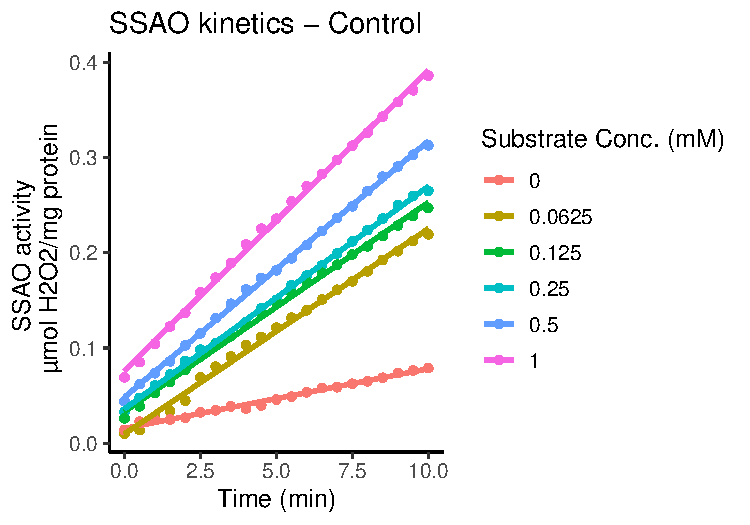
\includegraphics{results_files/figure-pdf/fig - ssao_activity_control-1.pdf}

}

\caption{SSAO activity measured over 10 minutes using benzylamine as
substrate}

\end{figure}%

The slope of these curves represents the initial velocity of each enzyme
reaction at different substrate concentrations and reported as
V\textsubscript{0} (µmol H\textsubscript{2}O\textsubscript{2}/min/mg
protein).

\begin{Shaded}
\begin{Highlighting}[]
\CommentTok{\#|}
\CommentTok{\# Creating a separate df for the control group for deriving initial velocity}

\NormalTok{kinetic\_data\_pivot\_control }\OtherTok{\textless{}{-}}\NormalTok{ kinetic\_data\_pivot }\SpecialCharTok{|\textgreater{}} \FunctionTok{filter}\NormalTok{(test\_group }\SpecialCharTok{==} \StringTok{"Control"}\NormalTok{)}


\CommentTok{\# lm modeling to generate slope for each substrate concentration}

\NormalTok{lm\_results }\OtherTok{\textless{}{-}}\NormalTok{ kinetic\_data\_pivot\_control }\SpecialCharTok{|\textgreater{}} 
  \FunctionTok{group\_by}\NormalTok{(substrate\_concn) }\SpecialCharTok{|\textgreater{}} 
  \FunctionTok{do}\NormalTok{(}\AttributeTok{model =} \FunctionTok{lm}\NormalTok{(ssao\_activity }\SpecialCharTok{\textasciitilde{}} \StringTok{\textasciigrave{}}\AttributeTok{Time (min)}\StringTok{\textasciigrave{}}\NormalTok{, }\AttributeTok{data =}\NormalTok{ .)) }\SpecialCharTok{|\textgreater{}} 
  \FunctionTok{mutate}\NormalTok{(}
  \AttributeTok{intercept =} \FunctionTok{coef}\NormalTok{(model)[[}\DecValTok{1}\NormalTok{]],}
  \AttributeTok{slope =} \FunctionTok{coef}\NormalTok{(model)[[}\DecValTok{2}\NormalTok{]],}
  \AttributeTok{equation =} \FunctionTok{sprintf}\NormalTok{(}\StringTok{"y = \%.4fx + \%.4f"}\NormalTok{, slope, intercept))}

\CommentTok{\# SSAO activity {-} initial velocity printed into a separate df}
\NormalTok{ssao\_control\_Vo }\OtherTok{\textless{}{-}} \FunctionTok{select}\NormalTok{(lm\_results, substrate\_concn, slope)}

\CommentTok{\# renaming the columns to S and V for easier use}
\NormalTok{ssao\_control\_Vo }\OtherTok{\textless{}{-}}\NormalTok{ ssao\_control\_Vo }\SpecialCharTok{|\textgreater{}} 
  \FunctionTok{rename}\NormalTok{(}\FunctionTok{c}\NormalTok{(}\StringTok{\textquotesingle{}V\textquotesingle{}} \OtherTok{=}\NormalTok{ slope, }\StringTok{\textquotesingle{}S\textquotesingle{}} \OtherTok{=}\NormalTok{ substrate\_concn))}

\NormalTok{table\_ssao\_control\_iniV }\OtherTok{\textless{}{-}}\NormalTok{ ssao\_control\_Vo }\SpecialCharTok{|\textgreater{}} 
  \FunctionTok{rename}\NormalTok{(}\FunctionTok{c}\NormalTok{(}\StringTok{\textquotesingle{}Initial Velocity\textquotesingle{}} \OtherTok{=} \StringTok{"V"}\NormalTok{, }
           \StringTok{\textquotesingle{}Substrate concentration\textquotesingle{}} \OtherTok{=} \StringTok{"S"}\NormalTok{))}
\FunctionTok{kable}\NormalTok{(}\FunctionTok{tibble}\NormalTok{(table\_ssao\_control\_iniV), }\AttributeTok{format =} \StringTok{"html"}\NormalTok{, }\AttributeTok{align =} \StringTok{"c"}\NormalTok{)}
\end{Highlighting}
\end{Shaded}

\begin{longtable}[]{@{}cc@{}}

\toprule\noalign{}
Substrate concentration & Initial Velocity \\
\midrule\noalign{}
\endhead
\bottomrule\noalign{}
\endlastfoot
0.0000 & 0.0062583 \\
0.0625 & 0.0215376 \\
0.1250 & 0.0219468 \\
0.2500 & 0.0233723 \\
0.5000 & 0.0268804 \\
1.0000 & 0.0315220 \\

\caption{\label{tbl-iniV}Initial Velocity for ssao activity for each
substrate concentration calculated by linear regression.}

\tabularnewline

\end{longtable}

The initial velocity for each substrate concentration was tabulated and
analysed using non-linear regression Michaelis-Menten kinetic model
(Equation~\ref{eq-mm}) to generate the Michaelis-Menten curve
Figure~\ref{fig-mmplot} and determine Km for benzylamine and Vmax values
(A. 2005).

\begin{Shaded}
\begin{Highlighting}[]
\CommentTok{\# Kinetic modelling to produce mm plots}

\CommentTok{\# Define the Michaelis{-}Menten equation}
\NormalTok{mm\_equation }\OtherTok{\textless{}{-}} \ControlFlowTok{function}\NormalTok{(S, Vm, Km) \{}
\NormalTok{  (Vm }\SpecialCharTok{*}\NormalTok{ S) }\SpecialCharTok{/}\NormalTok{ (Km }\SpecialCharTok{+}\NormalTok{ S)}
\NormalTok{\}}

\CommentTok{\# non{-}linear fitting}
\NormalTok{mm\_fit }\OtherTok{\textless{}{-}} \FunctionTok{nls}\NormalTok{(V}\SpecialCharTok{\textasciitilde{}} \FunctionTok{mm\_equation}\NormalTok{(S, Vm, Km),}
              \AttributeTok{data =}\NormalTok{ ssao\_control\_Vo,}
              \AttributeTok{start =} \FunctionTok{list}\NormalTok{(}\AttributeTok{Vm =} \FunctionTok{max}\NormalTok{(ssao\_control\_Vo}\SpecialCharTok{$}\NormalTok{V), }\AttributeTok{Km =} \FunctionTok{median}\NormalTok{(ssao\_control\_Vo}\SpecialCharTok{$}\NormalTok{S)))}

\CommentTok{\# Extracting the calculated parameters from above model}
\NormalTok{params }\OtherTok{\textless{}{-}} \FunctionTok{summary}\NormalTok{(mm\_fit)}\SpecialCharTok{$}\NormalTok{parameters}
\NormalTok{Km     }\OtherTok{\textless{}{-}}\NormalTok{ params[}\StringTok{"Km"}\NormalTok{, }\StringTok{"Estimate"}\NormalTok{]}
\NormalTok{Vm     }\OtherTok{\textless{}{-}}\NormalTok{ params[}\StringTok{"Vm"}\NormalTok{, }\StringTok{"Estimate"}\NormalTok{]}
\NormalTok{Vm\_se  }\OtherTok{\textless{}{-}}\NormalTok{ params[}\StringTok{"Vm"}\NormalTok{, }\StringTok{"Std. Error"}\NormalTok{]}
\NormalTok{Km\_se  }\OtherTok{\textless{}{-}}\NormalTok{ params[}\StringTok{"Km"}\NormalTok{, }\StringTok{"Std. Error"}\NormalTok{]}

\CommentTok{\# Generating points for the fitted curve}
\NormalTok{S\_curve }\OtherTok{\textless{}{-}} \FunctionTok{seq}\NormalTok{(}\DecValTok{0}\NormalTok{, }\FunctionTok{max}\NormalTok{(ssao\_control\_Vo}\SpecialCharTok{$}\NormalTok{S), }\AttributeTok{length.out =} \DecValTok{100}\NormalTok{)}
\NormalTok{V\_curve }\OtherTok{\textless{}{-}} \FunctionTok{predict}\NormalTok{(mm\_fit, }\AttributeTok{newdata =} \FunctionTok{list}\NormalTok{(}\AttributeTok{S =}\NormalTok{ S\_curve))}

\CommentTok{\# mm\_plot generation}
\FunctionTok{ggplot}\NormalTok{(ssao\_control\_Vo, }\FunctionTok{aes}\NormalTok{(}\AttributeTok{x =}\NormalTok{ S, }\AttributeTok{y =}\NormalTok{ V)) }\SpecialCharTok{+}
  \FunctionTok{geom\_point}\NormalTok{(}\AttributeTok{size =} \DecValTok{3}\NormalTok{)}\SpecialCharTok{+}
  \FunctionTok{geom\_line}\NormalTok{(}\AttributeTok{data =} \FunctionTok{data.frame}\NormalTok{(}\AttributeTok{S =}\NormalTok{ S\_curve, }\AttributeTok{V =}\NormalTok{ V\_curve), }\AttributeTok{color =} \StringTok{"blue"}\NormalTok{)}\SpecialCharTok{+}
  \FunctionTok{labs}\NormalTok{(}\AttributeTok{title =} \StringTok{"Micheales{-}Menten plot for SSAO kinetics"}\NormalTok{,}
       \AttributeTok{x =} \StringTok{"Substrate Concentration (mM)"}\NormalTok{,}
       \AttributeTok{y =} \StringTok{"Initial Velocity }\SpecialCharTok{\textbackslash{}n}\StringTok{ (µmol H2O2/min/mg protein)"}\NormalTok{)}\SpecialCharTok{+}
  \FunctionTok{theme\_classic2}\NormalTok{()}\SpecialCharTok{+}
  \FunctionTok{annotate}\NormalTok{(}\StringTok{"text"}\NormalTok{, }\AttributeTok{x =} \FunctionTok{max}\NormalTok{(ssao\_control\_Vo}\SpecialCharTok{$}\NormalTok{S), }\AttributeTok{y =} \FunctionTok{min}\NormalTok{(ssao\_control\_Vo}\SpecialCharTok{$}\NormalTok{V),}
           \AttributeTok{label =} \FunctionTok{sprintf}\NormalTok{(}\StringTok{"Vmax = \%.4f ± \%.4f µmol H2O2/min}
\StringTok{                           }\SpecialCharTok{\textbackslash{}n}\StringTok{Km = \%.4f ± \%.4f mM"}\NormalTok{, }
\NormalTok{                           Vm, Vm\_se, Km, Km\_se),}
           \AttributeTok{hjust =} \DecValTok{1}\NormalTok{, }\AttributeTok{vjust =} \DecValTok{0}\NormalTok{)}
\end{Highlighting}
\end{Shaded}

\begin{figure}[H]

\centering{

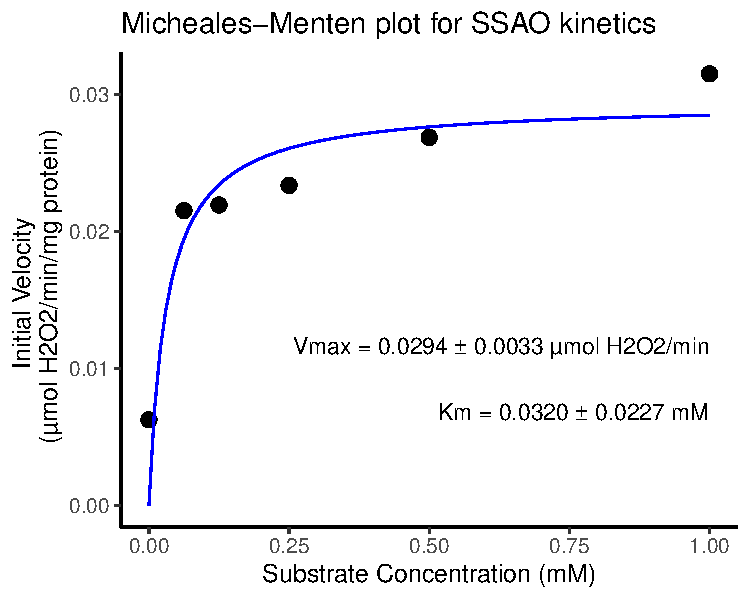
\includegraphics{results_files/figure-pdf/fig-mmplot-1.pdf}

}

\caption{\label{fig-mmplot}Micheales Menten plot for SSAO enzyme
kinetics using benzylamine as substrate}

\end{figure}%

From the nonlinear Michaelis Menten kinetic model, the Km and Vmax
values were determined to be 0.03193mM and 0.02941 µmol
H\textsubscript{2}O\textsubscript{2}/min, respectively.

\section{\texorpdfstring{\textbf{Enzyme
Inhibition}}{Enzyme Inhibition}}\label{enzyme-inhibition}

A key objective of this project is to measure the influence of caffeine
and simvastatin on SSAO activity. 10mM caffeine stock solution was
prepared by dissolving 19.4mg of caffeine in 10ml of
dH\textsubscript{2}O. Further dilutions of 1 and 0.1 mM were prepared
from the 10Mm stock solution and were used to in the kinetic
experiments. Similarly, 100mM simvastatin stock was prepared by directly
adding 4.78ml of DMSO to the vial containing 200mg of simvastatin
powder. 10, 1, and 0.1mM dilutions of simvastatin were prepared from the
100mM stock solution.

To study the effect of these inhibitors, 10µL of each inhibitor at
different concentrations were added to wells containing 60µL of SSAO
extract prepared by Method B (Experiment 1) in triplicate. The plates
were incubated at 37℃ prior to adding the reaction mixtures containing
different concentrations of the substrate.

The enzyme activity was initiated by adding the reaction mixtures the
containing substrate and the fluorescence measurements were started as
quickly as possible. The fluorescence values of control samples without
inhibitors, and samples containing inhibitors were measured every 30
seconds for 10 minutes. This data was exported to excel and was
formatted for further analysis. The fluorescence readings were converted
to equivalent H\textsubscript{2}O\textsubscript{2} concentrations using
the resorufin standard curve equation. These values were plotted against
time in minutes to obtain the initial velocity. The rate of hydrogen
peroxide formation is provided in the appendix1 for all the kinetic
experiments performed without and with different concentrations of the
inhibitors. The initial velocity of each group of substrate
concentrations with and without inhibitors were transferred to GraphPad
to plot a nonlinear regression curve using the competitive inhibition
kinetic model. This analysis was performed to calculate the Ki, Km, and
Vmax of the inhibition reaction. The nonlinear regression model for
competitive inhibition uses the following equation (A. 2005):

\begin{equation}\phantomsection\label{eq-nlm-CI}{
Km obs = Km*{(1+\frac{[I]}{Ki})}
}\end{equation}

\[
Y = \frac{Vmax*X}{Kmobs + X}
\]

Two-way ANOVA and Ad-Hoc Tukey's comparison was performed to compare the
difference in kinetic velocity between control and samples treated with
different concentrations of the inhibitor. A significant difference in
the initial velocities between different concentrations of the inhibitor
and the control is represented with a p-value less than 0.05.

\subsection{SSAO inhibition by
Simvastatin}\label{ssao-inhibition-by-simvastatin}

From the competitive inhibition model Equation~\ref{eq-nlm-CI} , the
K\textsubscript{i} for simvastatin was calculated to be 2.145 mM and the
K\textsubscript{m} and V\textsubscript{max} for benzylamine on SSAO were
0.01893 mM and 0.02385 µM H\textsubscript{2}O\textsubscript{2}/min
respectively ( Figure~\ref{fig-SIM-CI} ,
Table~\ref{tbl-sim-nlm-parameters} ). The initial velocities for each
simvastatin-treated SSAO sample were determined by performing linear
regression on the curve of H₂O₂ formation over time, as illustrated in
Figure~\ref{fig-ssao-sim-activity} and Table~\ref{tbl-sim-ini-v} .

\begin{Shaded}
\begin{Highlighting}[]
\NormalTok{kinetic\_data\_pivot }\SpecialCharTok{|\textgreater{}} 
  \FunctionTok{group\_by}\NormalTok{(test\_group) }\SpecialCharTok{|\textgreater{}} 
  \FunctionTok{filter}\NormalTok{(test\_group }\SpecialCharTok{==} \StringTok{"SIM"}\NormalTok{) }\SpecialCharTok{|\textgreater{}} 
  \FunctionTok{mutate}\NormalTok{(}\AttributeTok{substrate\_concn =} \FunctionTok{factor}\NormalTok{(substrate\_concn)) }\SpecialCharTok{|\textgreater{}} 
  \FunctionTok{ggplot}\NormalTok{(}\FunctionTok{aes}\NormalTok{(}\AttributeTok{x =} \StringTok{\textasciigrave{}}\AttributeTok{Time (min)}\StringTok{\textasciigrave{}}\NormalTok{, }
             \AttributeTok{y =}\NormalTok{ ssao\_activity, }
             \AttributeTok{color =}\NormalTok{ substrate\_concn, }
             \AttributeTok{group =}\NormalTok{ substrate\_concn))}\SpecialCharTok{+} 
  \FunctionTok{geom\_point}\NormalTok{() }\SpecialCharTok{+} 
  \FunctionTok{geom\_smooth}\NormalTok{(}\AttributeTok{method =}\NormalTok{ lm, }\AttributeTok{se =} \ConstantTok{FALSE}\NormalTok{)}\SpecialCharTok{+} 
  \FunctionTok{scale\_x\_continuous}\NormalTok{(}\AttributeTok{breaks =} \FunctionTok{c}\NormalTok{(}\DecValTok{0}\NormalTok{,}\DecValTok{5}\NormalTok{,}\DecValTok{10}\NormalTok{))}\SpecialCharTok{+}
  \FunctionTok{labs}\NormalTok{(}\AttributeTok{title =} \StringTok{"SSAO activity in the presence of 0.1, 1, and 10mM simvastatin"}\NormalTok{,}
       \AttributeTok{y =} \StringTok{"SSAO activity }\SpecialCharTok{\textbackslash{}n}\StringTok{ µmol H2O2/mg protein"}\NormalTok{,}
       \AttributeTok{color =} \StringTok{"Substrate Concn. (mM)"}\NormalTok{)}\SpecialCharTok{+}
  \FunctionTok{facet\_wrap}\NormalTok{(}\SpecialCharTok{\textasciitilde{}}\NormalTok{ inhibitor\_concn)}\SpecialCharTok{+}
  \FunctionTok{theme\_classic2}\NormalTok{()}\SpecialCharTok{+}
  \FunctionTok{theme}\NormalTok{(}\AttributeTok{legend.position =} \StringTok{"right"}\NormalTok{)}\SpecialCharTok{+}
  \FunctionTok{theme}\NormalTok{(}
    \AttributeTok{plot.title =} \FunctionTok{element\_text}\NormalTok{(}\AttributeTok{size =} \DecValTok{10}\NormalTok{, }\AttributeTok{hjust =} \FloatTok{0.5}\NormalTok{),}
    \AttributeTok{axis.title.y =} \FunctionTok{element\_text}\NormalTok{(}\AttributeTok{size =} \DecValTok{10}\NormalTok{, }\AttributeTok{margin =} \FunctionTok{margin}\NormalTok{(}\AttributeTok{t =} \DecValTok{0}\NormalTok{, }\AttributeTok{r =} \DecValTok{15}\NormalTok{, }\AttributeTok{b =} \DecValTok{0}\NormalTok{, }\AttributeTok{l =} \DecValTok{0}\NormalTok{)),}
    \AttributeTok{axis.text.x =} \FunctionTok{element\_text}\NormalTok{(}\AttributeTok{size =} \DecValTok{10}\NormalTok{),}
    \AttributeTok{axis.text.y =} \FunctionTok{element\_text}\NormalTok{(}\AttributeTok{size =} \DecValTok{10}\NormalTok{),}
    \AttributeTok{legend.title =} \FunctionTok{element\_text}\NormalTok{(}\AttributeTok{size =} \DecValTok{8}\NormalTok{),}
    \AttributeTok{legend.text =} \FunctionTok{element\_text}\NormalTok{(}\AttributeTok{size =} \DecValTok{6}\NormalTok{),}
    \AttributeTok{plot.margin =} \FunctionTok{margin}\NormalTok{(}\DecValTok{10}\NormalTok{, }\DecValTok{10}\NormalTok{,}\DecValTok{10}\NormalTok{, }\DecValTok{10}\NormalTok{)}
\NormalTok{  )}\SpecialCharTok{+}
  \FunctionTok{guides}\NormalTok{(}\AttributeTok{colour =} \FunctionTok{guide\_legend}\NormalTok{(}\AttributeTok{ncol =} \DecValTok{1}\NormalTok{, }\AttributeTok{position =} \StringTok{"right"}\NormalTok{))}
\end{Highlighting}
\end{Shaded}

\begin{figure}[H]

\centering{

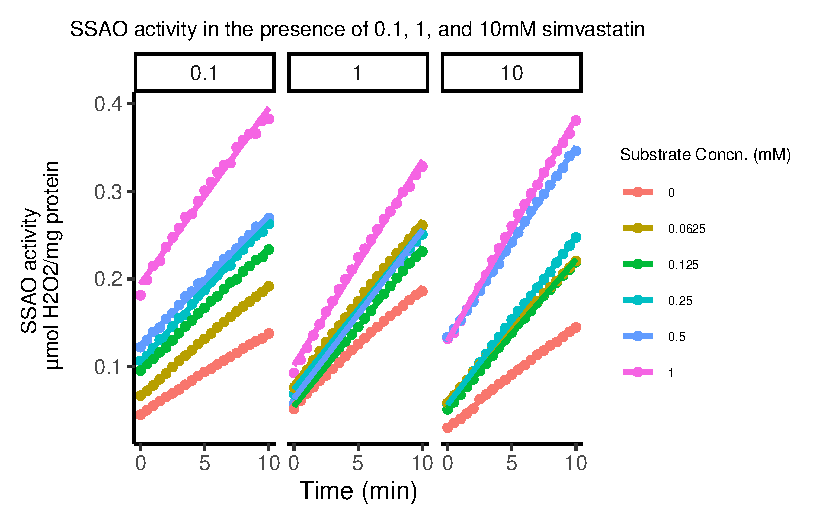
\includegraphics{results_files/figure-pdf/fig-ssao-sim-activity-1.pdf}

}

\caption{\label{fig-ssao-sim-activity}SSAO activity measured over 10
minutes with benzylamine as a substrate (1, 0.5, 0.25, 0.125, 0.0625mM)
and in the presence of simvastatin (SIM) at 0.1, 1, 10mM concentration.
SSAO activity is presented as µM H2O2/mg protein. A -- SSAO activity in
presence of 0.1mM SIM, B -- SSAO activity in the presence of 1mM SIM, C
-- SSAO activity in the presence of 10mM SIM.}

\end{figure}%

\begin{Shaded}
\begin{Highlighting}[]
\NormalTok{kinetic\_data\_pivot\_sim }\OtherTok{\textless{}{-}}\NormalTok{ kinetic\_data\_pivot }\SpecialCharTok{|\textgreater{}} \FunctionTok{filter}\NormalTok{(test\_group }\SpecialCharTok{==} \StringTok{"SIM"}\NormalTok{)}


\CommentTok{\# lm modeling to generate slope for each substrate concentration}

\NormalTok{lm\_results\_sim }\OtherTok{\textless{}{-}}\NormalTok{ kinetic\_data\_pivot\_sim }\SpecialCharTok{|\textgreater{}} 
  \FunctionTok{group\_by}\NormalTok{(substrate\_concn, inhibitor\_concn) }\SpecialCharTok{|\textgreater{}} 
  \FunctionTok{do}\NormalTok{(}\AttributeTok{model =} \FunctionTok{lm}\NormalTok{(ssao\_activity }\SpecialCharTok{\textasciitilde{}} \StringTok{\textasciigrave{}}\AttributeTok{Time (min)}\StringTok{\textasciigrave{}}\NormalTok{, }\AttributeTok{data =}\NormalTok{ .)) }\SpecialCharTok{|\textgreater{}} 
  \FunctionTok{mutate}\NormalTok{(}
  \AttributeTok{intercept =} \FunctionTok{coef}\NormalTok{(model)[[}\DecValTok{1}\NormalTok{]],}
  \AttributeTok{slope =} \FunctionTok{coef}\NormalTok{(model)[[}\DecValTok{2}\NormalTok{]],}
  \AttributeTok{equation =} \FunctionTok{sprintf}\NormalTok{(}\StringTok{"y = \%.4fx + \%.4f"}\NormalTok{, slope, intercept))}

\NormalTok{lm\_results\_sim }\SpecialCharTok{|\textgreater{}} \FunctionTok{pivot\_wider}\NormalTok{(}
  \AttributeTok{id\_cols =}\NormalTok{ substrate\_concn,}
  \AttributeTok{names\_from =}\NormalTok{ inhibitor\_concn,}
  \AttributeTok{values\_from =}\NormalTok{ slope}
\NormalTok{) }\SpecialCharTok{|\textgreater{}} \FunctionTok{rename}\NormalTok{(}\StringTok{\textquotesingle{}Substrate Concentration (mM)\textquotesingle{}} \OtherTok{=} \StringTok{"substrate\_concn"}\NormalTok{,}
            \StringTok{\textquotesingle{}SIM 10 mM\textquotesingle{}} \OtherTok{=} \StringTok{"0.1"}\NormalTok{,}
            \StringTok{\textquotesingle{}SIM 1 mM\textquotesingle{}} \OtherTok{=} \StringTok{"1"}\NormalTok{,}
            \StringTok{\textquotesingle{}SIM 0.1 mM\textquotesingle{}} \OtherTok{=} \StringTok{"10"}
\NormalTok{            ) }\SpecialCharTok{|\textgreater{}} \FunctionTok{kable}\NormalTok{(}\AttributeTok{align =} \StringTok{"c"}\NormalTok{)}
\end{Highlighting}
\end{Shaded}

\begin{longtable}[]{@{}cccc@{}}

\toprule\noalign{}
Substrate Concentration (mM) & SIM 10 mM & SIM 1 mM & SIM 0.1 mM \\
\midrule\noalign{}
\endhead
\bottomrule\noalign{}
\endlastfoot
0.0000 & 0.0091990 & 0.0133830 & 0.0115535 \\
0.0625 & 0.0125717 & 0.0185989 & 0.0161799 \\
0.1250 & 0.0139309 & 0.0180983 & 0.0169519 \\
0.2500 & 0.0159289 & 0.0181323 & 0.0190872 \\
0.5000 & 0.0147374 & 0.0191430 & 0.0217997 \\
1.0000 & 0.0200087 & 0.0232822 & 0.0254066 \\

\caption{\label{tbl-sim-ini-v}Initial velocities of SSAO activity in the
presence of simvastatin at 0.1, 1, and 1mM concentrations.}

\tabularnewline

\end{longtable}

\begin{Shaded}
\begin{Highlighting}[]
\FunctionTok{library}\NormalTok{(minpack.lm)}
\CommentTok{\# Create the dataset}
\NormalTok{data }\OtherTok{\textless{}{-}} \FunctionTok{data.frame}\NormalTok{(}
  \AttributeTok{S =} \FunctionTok{rep}\NormalTok{(}\FunctionTok{c}\NormalTok{(}\DecValTok{0}\NormalTok{, }\FloatTok{0.0625}\NormalTok{, }\FloatTok{0.125}\NormalTok{, }\FloatTok{0.25}\NormalTok{, }\FloatTok{0.5}\NormalTok{, }\DecValTok{1}\NormalTok{), }\AttributeTok{each =} \DecValTok{4}\NormalTok{),}
  \AttributeTok{I =} \FunctionTok{rep}\NormalTok{(}\FunctionTok{c}\NormalTok{(}\DecValTok{0}\NormalTok{, }\DecValTok{10}\NormalTok{, }\DecValTok{1}\NormalTok{, }\FloatTok{0.1}\NormalTok{)),}
  \AttributeTok{V =} \FunctionTok{c}\NormalTok{(}\FloatTok{0.006258}\NormalTok{, }\FloatTok{0.01155}\NormalTok{, }\FloatTok{0.01338}\NormalTok{, }\FloatTok{0.009199}\NormalTok{,}
        \FloatTok{0.02154}\NormalTok{, }\FloatTok{0.01257}\NormalTok{, }\FloatTok{0.0186}\NormalTok{, }\FloatTok{0.01618}\NormalTok{,}
        \FloatTok{0.02195}\NormalTok{, }\FloatTok{0.01393}\NormalTok{, }\FloatTok{0.0181}\NormalTok{, }\FloatTok{0.01695}\NormalTok{,}
        \FloatTok{0.02337}\NormalTok{, }\FloatTok{0.01593}\NormalTok{, }\FloatTok{0.01813}\NormalTok{, }\FloatTok{0.01909}\NormalTok{,}
        \FloatTok{0.02688}\NormalTok{, }\FloatTok{0.01474}\NormalTok{, }\FloatTok{0.01914}\NormalTok{, }\FloatTok{0.0218}\NormalTok{,}
        \FloatTok{0.03152}\NormalTok{, }\FloatTok{0.02001}\NormalTok{, }\FloatTok{0.02328}\NormalTok{, }\FloatTok{0.02541}\NormalTok{))}

\CommentTok{\# Define the competitive inhibition model function using GraphPad\textquotesingle{}s equation}
\NormalTok{comp\_inhib }\OtherTok{\textless{}{-}} \ControlFlowTok{function}\NormalTok{(S, I, Vmax, Km, Ki) \{}
\NormalTok{  Km\_obs }\OtherTok{\textless{}{-}}\NormalTok{ Km }\SpecialCharTok{*}\NormalTok{ (}\DecValTok{1} \SpecialCharTok{+}\NormalTok{ I }\SpecialCharTok{/}\NormalTok{ Ki)}
\NormalTok{  (Vmax }\SpecialCharTok{*}\NormalTok{ S) }\SpecialCharTok{/}\NormalTok{ (Km\_obs }\SpecialCharTok{+}\NormalTok{ S)}
\NormalTok{\}}

\CommentTok{\# Set initial parameter values (using GraphPad\textquotesingle{}s results)}
\NormalTok{start\_vals }\OtherTok{\textless{}{-}} \FunctionTok{list}\NormalTok{(}\AttributeTok{Vmax =} \FloatTok{0.1}\NormalTok{, }\AttributeTok{Km =} \FloatTok{0.1}\NormalTok{, }\AttributeTok{Ki =} \FloatTok{0.1}\NormalTok{)}

\CommentTok{\# Fit the model using nlsLM for more robust fitting}
\NormalTok{sim\_fit }\OtherTok{\textless{}{-}} \FunctionTok{nlsLM}\NormalTok{(V }\SpecialCharTok{\textasciitilde{}} \FunctionTok{comp\_inhib}\NormalTok{(S, I, Vmax, Km, Ki), }
             \AttributeTok{data =}\NormalTok{ data, }
             \AttributeTok{start =}\NormalTok{ start\_vals,}
             \AttributeTok{lower =} \FunctionTok{c}\NormalTok{(}\AttributeTok{Vmax =} \DecValTok{0}\NormalTok{, }\AttributeTok{Km =} \DecValTok{0}\NormalTok{, }\AttributeTok{Ki =} \DecValTok{0}\NormalTok{),}
             \AttributeTok{control =} \FunctionTok{nls.lm.control}\NormalTok{(}\AttributeTok{maxiter =} \DecValTok{1000}\NormalTok{, }\AttributeTok{maxfev =} \DecValTok{1000}\NormalTok{))}

\CommentTok{\# Extract the fitted parameters}
\NormalTok{sim\_params }\OtherTok{\textless{}{-}} \FunctionTok{coef}\NormalTok{(sim\_fit)}
\NormalTok{sim\_summary\_fit }\OtherTok{\textless{}{-}} \FunctionTok{summary}\NormalTok{(sim\_fit)}


\CommentTok{\# Calculate R{-}squared}
\NormalTok{ss\_total }\OtherTok{\textless{}{-}} \FunctionTok{sum}\NormalTok{((data}\SpecialCharTok{$}\NormalTok{V }\SpecialCharTok{{-}} \FunctionTok{mean}\NormalTok{(data}\SpecialCharTok{$}\NormalTok{V))}\SpecialCharTok{\^{}}\DecValTok{2}\NormalTok{)}
\NormalTok{ss\_residual }\OtherTok{\textless{}{-}} \FunctionTok{sum}\NormalTok{(}\FunctionTok{residuals}\NormalTok{(sim\_fit)}\SpecialCharTok{\^{}}\DecValTok{2}\NormalTok{)}
\NormalTok{r\_squared }\OtherTok{\textless{}{-}} \DecValTok{1} \SpecialCharTok{{-}}\NormalTok{ (ss\_residual }\SpecialCharTok{/}\NormalTok{ ss\_total)}

\NormalTok{sim\_nlm\_values }\OtherTok{\textless{}{-}} \FunctionTok{c}\NormalTok{(}
\NormalTok{Km }\OtherTok{\textless{}{-}} \FunctionTok{sprintf}\NormalTok{(}\StringTok{"\%.5f"}\NormalTok{, sim\_params[}\StringTok{"Km"}\NormalTok{]),}
\NormalTok{Vmax }\OtherTok{\textless{}{-}} \FunctionTok{sprintf}\NormalTok{(}\StringTok{"\%.5f"}\NormalTok{, sim\_params[}\StringTok{"Vmax"}\NormalTok{]),}
\NormalTok{Ki }\OtherTok{\textless{}{-}} \FunctionTok{sprintf}\NormalTok{(}\StringTok{"\%.5f"}\NormalTok{, sim\_params[}\StringTok{"Ki"}\NormalTok{]),}
\NormalTok{r\_squaredv }\OtherTok{\textless{}{-}} \FunctionTok{sprintf}\NormalTok{(}\StringTok{"\%.5f"}\NormalTok{, r\_squared))}



\CommentTok{\# MM Plot}
\FunctionTok{ggplot}\NormalTok{(data, }\FunctionTok{aes}\NormalTok{(}\AttributeTok{x =}\NormalTok{ S, }\AttributeTok{y =}\NormalTok{ V, }\AttributeTok{color =} \FunctionTok{factor}\NormalTok{(I))) }\SpecialCharTok{+}
  \FunctionTok{geom\_point}\NormalTok{(}\AttributeTok{size =} \DecValTok{3}\NormalTok{) }\SpecialCharTok{+}
  \FunctionTok{geom\_line}\NormalTok{(}\AttributeTok{data =} \FunctionTok{data.frame}\NormalTok{(}\AttributeTok{S =} \FunctionTok{rep}\NormalTok{(}\FunctionTok{seq}\NormalTok{(}\DecValTok{0}\NormalTok{, }\FunctionTok{max}\NormalTok{(data}\SpecialCharTok{$}\NormalTok{S), }\AttributeTok{length.out =} \DecValTok{100}\NormalTok{), }\DecValTok{4}\NormalTok{),}
                              \AttributeTok{I =} \FunctionTok{rep}\NormalTok{(}\FunctionTok{c}\NormalTok{(}\DecValTok{0}\NormalTok{, }\FloatTok{0.1}\NormalTok{, }\DecValTok{1}\NormalTok{, }\DecValTok{10}\NormalTok{), }\AttributeTok{each =} \DecValTok{100}\NormalTok{)) }\SpecialCharTok{|\textgreater{}} 
              \FunctionTok{mutate}\NormalTok{(}\AttributeTok{V =} \FunctionTok{comp\_inhib}\NormalTok{(S, I, sim\_params[}\StringTok{"Vmax"}\NormalTok{], }
\NormalTok{                                    sim\_params[}\StringTok{"Km"}\NormalTok{], }
\NormalTok{                                    sim\_params[}\StringTok{"Ki"}\NormalTok{])),}
            \FunctionTok{aes}\NormalTok{(}\AttributeTok{x =}\NormalTok{ S, }\AttributeTok{y =}\NormalTok{ V, }\AttributeTok{color =} \FunctionTok{factor}\NormalTok{(I))) }\SpecialCharTok{+}
  \FunctionTok{labs}\NormalTok{(}\AttributeTok{title =} \StringTok{"Competitive Inhibition of SSAO by simvastatin"}\NormalTok{,}
       \AttributeTok{x =} \StringTok{"Substrate Concentration (mM)"}\NormalTok{,}
       \AttributeTok{y =} \StringTok{"Initial Velocity }\SpecialCharTok{\textbackslash{}n}\StringTok{(µmol H2O2/min/mg protein)"}\NormalTok{,}
       \AttributeTok{color =} \StringTok{"Simvastatin Concentration (mM)"}\NormalTok{) }\SpecialCharTok{+}
  \FunctionTok{theme\_classic2}\NormalTok{() }\SpecialCharTok{+}
  \FunctionTok{scale\_color\_brewer}\NormalTok{(}\AttributeTok{palette =} \StringTok{"Set1"}\NormalTok{)}\SpecialCharTok{+}
  \FunctionTok{annotate}\NormalTok{(}\StringTok{"text"}\NormalTok{, }
           \AttributeTok{x =} \FloatTok{0.75}\NormalTok{, }\AttributeTok{y =} \FloatTok{0.01}\NormalTok{,}
           \AttributeTok{label =} \FunctionTok{sprintf}\NormalTok{(}\StringTok{"Vmax = \%.4f}\SpecialCharTok{\textbackslash{}n}\StringTok{Km = \%.4f}\SpecialCharTok{\textbackslash{}n}\StringTok{ Ki = \%.4f"}\NormalTok{, }
\NormalTok{                           sim\_params[}\StringTok{"Vmax"}\NormalTok{], }
\NormalTok{                           sim\_params[}\StringTok{"Km"}\NormalTok{], }
\NormalTok{                           sim\_params[}\StringTok{"Ki"}\NormalTok{]))}\SpecialCharTok{+}
  \FunctionTok{theme}\NormalTok{(}\AttributeTok{legend.position =} \StringTok{"bottom"}\NormalTok{)}\SpecialCharTok{+}
  \FunctionTok{guides}\NormalTok{(}\AttributeTok{colour =} \FunctionTok{guide\_legend}\NormalTok{(}\AttributeTok{nrow =} \DecValTok{1}\NormalTok{))}
\end{Highlighting}
\end{Shaded}

\begin{figure}[H]

\centering{

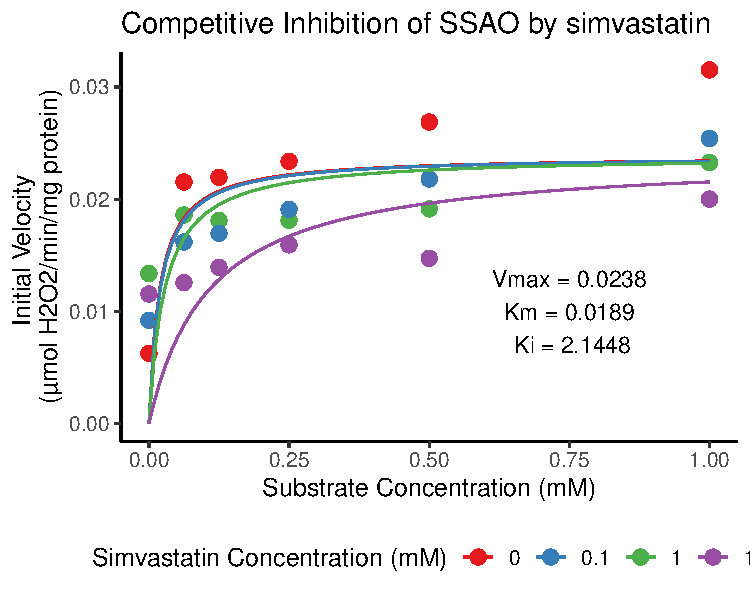
\includegraphics{results_files/figure-pdf/fig-SIM-CI-1.pdf}

}

\caption{\label{fig-SIM-CI}SSAO inhibition by simvastatin calculated by
non-linear competetive inhibition model}

\end{figure}%

\begin{Shaded}
\begin{Highlighting}[]
\NormalTok{sim\_ssao\_nlm\_results }\OtherTok{\textless{}{-}} \FunctionTok{tibble}\NormalTok{(}\AttributeTok{Parameters\_SIM\_SSAO =} \FunctionTok{c}\NormalTok{(}\StringTok{"Km"}\NormalTok{, }\StringTok{"Vmax"}\NormalTok{, }\StringTok{"Ki"}\NormalTok{, }\StringTok{"R{-}squared"}\NormalTok{), }
                               \AttributeTok{Values =}\NormalTok{ sim\_nlm\_values)}
\FunctionTok{kable}\NormalTok{(sim\_ssao\_nlm\_results)}
\end{Highlighting}
\end{Shaded}

\begin{longtable}[]{@{}ll@{}}

\toprule\noalign{}
Parameters\_SIM\_SSAO & Values \\
\midrule\noalign{}
\endhead
\bottomrule\noalign{}
\endlastfoot
Km & 0.01893 \\
Vmax & 0.02385 \\
Ki & 2.14483 \\
R-squared & 0.17029 \\

\caption{\label{tbl-sim-nlm-parameters}Non linear fit parameters for
SSAO inhibition by simvastatin}

\tabularnewline

\end{longtable}

\subsection{SSAO inhibition by
Caffeine}\label{ssao-inhibition-by-caffeine}

Like simvastatin, caffeine also follows the competitive inhibition model
( Equation~\ref{eq-nlm-CI} ) and the K\textsubscript{i} for caffeine was
calculated from one independent experiment ( Figure~\ref{fig-CAF-CI} ).
The K\textsubscript{i} value for caffeine calculated from competitive
inhibition model is 6.768mM and the K\textsubscript{m} and
V\textsubscript{max} for benzylamine on SSAO were 0.02903mM and 0.02850
µM H\textsubscript{2}O\textsubscript{2}/min, respectively (
Figure~\ref{fig-CAF-CI} and Table~\ref{tbl-nlm-caf-fit} ).

\begin{Shaded}
\begin{Highlighting}[]
\NormalTok{kinetic\_data\_pivot }\SpecialCharTok{|\textgreater{}} 
  \FunctionTok{group\_by}\NormalTok{(test\_group) }\SpecialCharTok{|\textgreater{}} 
  \FunctionTok{filter}\NormalTok{(test\_group }\SpecialCharTok{==} \StringTok{"CAF"}\NormalTok{) }\SpecialCharTok{|\textgreater{}} 
  \FunctionTok{mutate}\NormalTok{(}\AttributeTok{substrate\_concn =} \FunctionTok{factor}\NormalTok{(substrate\_concn)) }\SpecialCharTok{|\textgreater{}} 
  \FunctionTok{ggplot}\NormalTok{(}\FunctionTok{aes}\NormalTok{(}\AttributeTok{x =} \StringTok{\textasciigrave{}}\AttributeTok{Time (min)}\StringTok{\textasciigrave{}}\NormalTok{, }
             \AttributeTok{y =}\NormalTok{ ssao\_activity, }
             \AttributeTok{color =}\NormalTok{ substrate\_concn, }
             \AttributeTok{group =}\NormalTok{ substrate\_concn))}\SpecialCharTok{+} 
  \FunctionTok{geom\_point}\NormalTok{() }\SpecialCharTok{+} 
  \FunctionTok{labs}\NormalTok{(}\AttributeTok{title =} \StringTok{"SSAO activity in the presence of 0.1, 1, and 10mM caffeine"}\NormalTok{,}
       \AttributeTok{y =} \StringTok{"SSAO activity }\SpecialCharTok{\textbackslash{}n}\StringTok{ µmol H2O2/mg protein"}\NormalTok{,}
       \AttributeTok{color =} \StringTok{"Substrate Concn. (mM)"}\NormalTok{)}\SpecialCharTok{+}
  \FunctionTok{geom\_smooth}\NormalTok{(}\AttributeTok{method =}\NormalTok{ lm, }\AttributeTok{se =} \ConstantTok{FALSE}\NormalTok{)}\SpecialCharTok{+} 
  \FunctionTok{facet\_wrap}\NormalTok{(}\SpecialCharTok{\textasciitilde{}}\NormalTok{ inhibitor\_concn)}\SpecialCharTok{+}
  \FunctionTok{scale\_x\_continuous}\NormalTok{(}\AttributeTok{breaks =} \FunctionTok{c}\NormalTok{(}\DecValTok{0}\NormalTok{,}\DecValTok{5}\NormalTok{,}\DecValTok{10}\NormalTok{))}\SpecialCharTok{+}
  \FunctionTok{theme\_classic2}\NormalTok{()}\SpecialCharTok{+}
  \FunctionTok{theme}\NormalTok{(}\AttributeTok{legend.position =} \StringTok{"right"}\NormalTok{)}\SpecialCharTok{+}
  \FunctionTok{theme}\NormalTok{(}
    \AttributeTok{plot.title =} \FunctionTok{element\_text}\NormalTok{(}\AttributeTok{size =} \DecValTok{10}\NormalTok{, }\AttributeTok{hjust =} \FloatTok{0.5}\NormalTok{),}
    \AttributeTok{axis.title.y =} \FunctionTok{element\_text}\NormalTok{(}\AttributeTok{size =} \DecValTok{10}\NormalTok{, }\AttributeTok{margin =} \FunctionTok{margin}\NormalTok{(}\AttributeTok{t =} \DecValTok{0}\NormalTok{, }\AttributeTok{r =} \DecValTok{15}\NormalTok{, }\AttributeTok{b =} \DecValTok{0}\NormalTok{, }\AttributeTok{l =} \DecValTok{0}\NormalTok{)),}
    \AttributeTok{axis.text.x =} \FunctionTok{element\_text}\NormalTok{(}\AttributeTok{size =} \DecValTok{10}\NormalTok{),}
    \AttributeTok{axis.text.y =} \FunctionTok{element\_text}\NormalTok{(}\AttributeTok{size =} \DecValTok{10}\NormalTok{),}
    \AttributeTok{legend.title =} \FunctionTok{element\_text}\NormalTok{(}\AttributeTok{size =} \DecValTok{8}\NormalTok{),}
    \AttributeTok{legend.text =} \FunctionTok{element\_text}\NormalTok{(}\AttributeTok{size =} \DecValTok{6}\NormalTok{),}
    \AttributeTok{plot.margin =} \FunctionTok{margin}\NormalTok{(}\DecValTok{8}\NormalTok{, }\DecValTok{8}\NormalTok{, }\DecValTok{8}\NormalTok{, }\DecValTok{8}\NormalTok{)}
\NormalTok{  )}\SpecialCharTok{+}
  \FunctionTok{guides}\NormalTok{(}\AttributeTok{colour =} \FunctionTok{guide\_legend}\NormalTok{(}\AttributeTok{ncol =} \DecValTok{1}\NormalTok{))}
\end{Highlighting}
\end{Shaded}

\begin{figure}[H]

\centering{

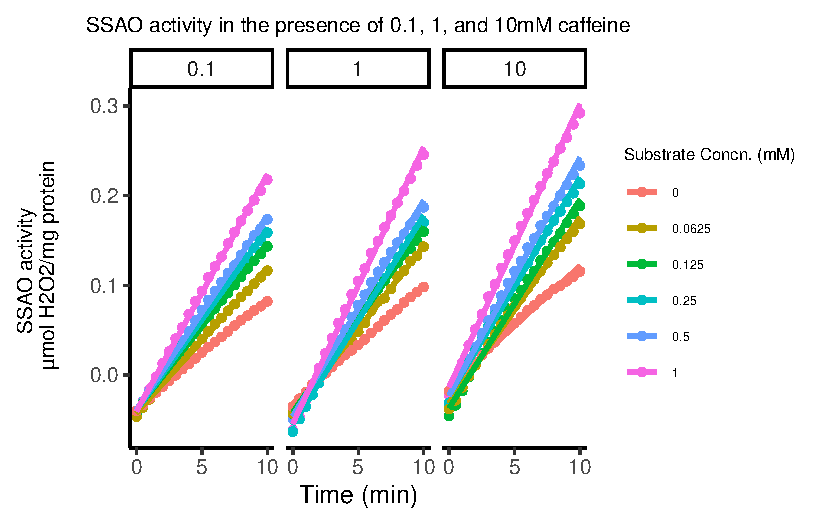
\includegraphics{results_files/figure-pdf/fig-ssao-activity-plot-caf-1.pdf}

}

\caption{\label{fig-ssao-activity-plot-caf}SSAO activity measured over
10 minutes with benzylamine as a substrate (1, 0.5, 0.25, 0.125,
0.0625mM) and in the presence of caffeine (CAF) at 0.1, 1, 10mM
concentration. SSAO activity is presented as µM H2O2/mg protein. A --
SSAO activity in presence of 0.1mM CAF, B -- SSAO activity in the
presence of 1mM CAF, C -- SSAO activity in the presence of 10mM CAF.}

\end{figure}%

\begin{Shaded}
\begin{Highlighting}[]
\NormalTok{kinetic\_data\_pivot\_caf }\OtherTok{\textless{}{-}}\NormalTok{ kinetic\_data\_pivot }\SpecialCharTok{|\textgreater{}} \FunctionTok{filter}\NormalTok{(test\_group }\SpecialCharTok{==} \StringTok{"CAF"}\NormalTok{)}


\CommentTok{\# lm modeling to generate slope for each substrate concentration}

\NormalTok{lm\_results\_caf }\OtherTok{\textless{}{-}}\NormalTok{ kinetic\_data\_pivot\_caf }\SpecialCharTok{|\textgreater{}} 
  \FunctionTok{group\_by}\NormalTok{(substrate\_concn, inhibitor\_concn) }\SpecialCharTok{|\textgreater{}} 
  \FunctionTok{do}\NormalTok{(}\AttributeTok{model =} \FunctionTok{lm}\NormalTok{(ssao\_activity }\SpecialCharTok{\textasciitilde{}} \StringTok{\textasciigrave{}}\AttributeTok{Time (min)}\StringTok{\textasciigrave{}}\NormalTok{, }\AttributeTok{data =}\NormalTok{ .)) }\SpecialCharTok{|\textgreater{}} 
  \FunctionTok{mutate}\NormalTok{(}
  \AttributeTok{intercept =} \FunctionTok{coef}\NormalTok{(model)[[}\DecValTok{1}\NormalTok{]],}
  \AttributeTok{slope =} \FunctionTok{coef}\NormalTok{(model)[[}\DecValTok{2}\NormalTok{]],}
  \AttributeTok{equation =} \FunctionTok{sprintf}\NormalTok{(}\StringTok{"y = \%.4fx + \%.4f"}\NormalTok{, slope, intercept))}

\NormalTok{lm\_results\_caf }\SpecialCharTok{|\textgreater{}} \FunctionTok{pivot\_wider}\NormalTok{(}
  \AttributeTok{id\_cols =}\NormalTok{ substrate\_concn,}
  \AttributeTok{names\_from =}\NormalTok{ inhibitor\_concn,}
  \AttributeTok{values\_from =}\NormalTok{ slope}
\NormalTok{) }\SpecialCharTok{|\textgreater{}} \FunctionTok{rename}\NormalTok{(}\StringTok{\textquotesingle{}Substrate Concentration (mM)\textquotesingle{}} \OtherTok{=} \StringTok{"substrate\_concn"}\NormalTok{,}
            \StringTok{\textquotesingle{}CAF 10 mM\textquotesingle{}} \OtherTok{=} \StringTok{"10"}\NormalTok{,}
            \StringTok{\textquotesingle{}CAF 1 mM\textquotesingle{}} \OtherTok{=} \StringTok{"1"}\NormalTok{,}
            \StringTok{\textquotesingle{}CAF 0.1 mM\textquotesingle{}} \OtherTok{=} \StringTok{"0.1"}
\NormalTok{            ) }\SpecialCharTok{|\textgreater{}} \FunctionTok{kable}\NormalTok{(}\AttributeTok{align =} \StringTok{"c"}\NormalTok{)}
\end{Highlighting}
\end{Shaded}

\begin{longtable}[]{@{}cccc@{}}

\toprule\noalign{}
Substrate Concentration (mM) & CAF 0.1 mM & CAF 1 mM & CAF 10 mM \\
\midrule\noalign{}
\endhead
\bottomrule\noalign{}
\endlastfoot
0.0000 & 0.0122429 & 0.0131826 & 0.0134182 \\
0.0625 & 0.0161367 & 0.0185402 & 0.0206733 \\
0.1250 & 0.0185621 & 0.0206289 & 0.0232647 \\
0.2500 & 0.0202061 & 0.0233087 & 0.0242922 \\
0.5000 & 0.0215960 & 0.0240157 & 0.0265001 \\
1.0000 & 0.0263826 & 0.0308273 & 0.0314966 \\

\caption{\label{tbl-caf-ini-v}Initial velocities of SSAO activity in the
presence of caffeine at 0.1, 1, and 1mM concentrations.}

\tabularnewline

\end{longtable}

\begin{Shaded}
\begin{Highlighting}[]
\FunctionTok{library}\NormalTok{(minpack.lm)  }\CommentTok{\# For more robust nonlinear fitting}

\CommentTok{\# Create the dataset}
\NormalTok{data }\OtherTok{\textless{}{-}} \FunctionTok{data.frame}\NormalTok{(}
  \AttributeTok{S =} \FunctionTok{rep}\NormalTok{(}\FunctionTok{c}\NormalTok{(}\DecValTok{0}\NormalTok{, }\FloatTok{0.0625}\NormalTok{, }\FloatTok{0.125}\NormalTok{, }\FloatTok{0.25}\NormalTok{, }\FloatTok{0.5}\NormalTok{, }\DecValTok{1}\NormalTok{), }\AttributeTok{each =} \DecValTok{4}\NormalTok{),}
  \AttributeTok{I =} \FunctionTok{rep}\NormalTok{(}\FunctionTok{c}\NormalTok{(}\DecValTok{0}\NormalTok{, }\FloatTok{0.1}\NormalTok{, }\DecValTok{1}\NormalTok{, }\DecValTok{10}\NormalTok{)),}
  \AttributeTok{V =} \FunctionTok{c}\NormalTok{(}\FloatTok{0.006258}\NormalTok{, }\FloatTok{0.01342}\NormalTok{, }\FloatTok{0.01318}\NormalTok{, }\FloatTok{0.01224}\NormalTok{,}
        \FloatTok{0.02154}\NormalTok{, }\FloatTok{0.02067}\NormalTok{, }\FloatTok{0.01854}\NormalTok{, }\FloatTok{0.01614}\NormalTok{,}
        \FloatTok{0.02195}\NormalTok{, }\FloatTok{0.02326}\NormalTok{, }\FloatTok{0.02063}\NormalTok{, }\FloatTok{0.01856}\NormalTok{,}
        \FloatTok{0.02337}\NormalTok{, }\FloatTok{0.02429}\NormalTok{, }\FloatTok{0.02331}\NormalTok{, }\FloatTok{0.02021}\NormalTok{,}
        \FloatTok{0.02688}\NormalTok{, }\FloatTok{0.0265}\NormalTok{, }\FloatTok{0.02402}\NormalTok{, }\FloatTok{0.0216}\NormalTok{,}
        \FloatTok{0.03152}\NormalTok{, }\FloatTok{0.0315}\NormalTok{, }\FloatTok{0.03083}\NormalTok{, }\FloatTok{0.02638}\NormalTok{))}

\CommentTok{\# Define the competitive inhibition model function using GraphPad\textquotesingle{}s equation}
\NormalTok{comp\_inhib }\OtherTok{\textless{}{-}} \ControlFlowTok{function}\NormalTok{(S, I, Vmax, Km, Ki) \{}
\NormalTok{  Km\_obs }\OtherTok{\textless{}{-}}\NormalTok{ Km }\SpecialCharTok{*}\NormalTok{ (}\DecValTok{1} \SpecialCharTok{+}\NormalTok{ I }\SpecialCharTok{/}\NormalTok{ Ki)}
\NormalTok{  (Vmax }\SpecialCharTok{*}\NormalTok{ S) }\SpecialCharTok{/}\NormalTok{ (Km\_obs }\SpecialCharTok{+}\NormalTok{ S)}
\NormalTok{\}}

\CommentTok{\# Set initial parameter values (using GraphPad\textquotesingle{}s results)}
\NormalTok{start\_vals }\OtherTok{\textless{}{-}} \FunctionTok{list}\NormalTok{(}\AttributeTok{Vmax =} \FloatTok{0.1}\NormalTok{, }\AttributeTok{Km =} \FloatTok{0.1}\NormalTok{, }\AttributeTok{Ki =} \FloatTok{0.1}\NormalTok{)}

\CommentTok{\# Fit the model using nlsLM for more robust fitting}
\NormalTok{fit }\OtherTok{\textless{}{-}} \FunctionTok{nlsLM}\NormalTok{(V }\SpecialCharTok{\textasciitilde{}} \FunctionTok{comp\_inhib}\NormalTok{(S, I, Vmax, Km, Ki), }
             \AttributeTok{data =}\NormalTok{ data, }
             \AttributeTok{start =}\NormalTok{ start\_vals,}
             \AttributeTok{lower =} \FunctionTok{c}\NormalTok{(}\AttributeTok{Vmax =} \DecValTok{0}\NormalTok{, }\AttributeTok{Km =} \DecValTok{0}\NormalTok{, }\AttributeTok{Ki =} \DecValTok{0}\NormalTok{),}
             \AttributeTok{control =} \FunctionTok{nls.lm.control}\NormalTok{(}\AttributeTok{maxiter =} \DecValTok{1000}\NormalTok{, }\AttributeTok{maxfev =} \DecValTok{1000}\NormalTok{))}

\CommentTok{\# Extract the fitted parameters}
\NormalTok{params }\OtherTok{\textless{}{-}} \FunctionTok{coef}\NormalTok{(fit)}
\NormalTok{summary\_fit }\OtherTok{\textless{}{-}} \FunctionTok{summary}\NormalTok{(fit)}
\CommentTok{\# R{-}squared}
\NormalTok{ss\_total }\OtherTok{\textless{}{-}} \FunctionTok{sum}\NormalTok{((data}\SpecialCharTok{$}\NormalTok{V }\SpecialCharTok{{-}} \FunctionTok{mean}\NormalTok{(data}\SpecialCharTok{$}\NormalTok{V))}\SpecialCharTok{\^{}}\DecValTok{2}\NormalTok{)}
\NormalTok{ss\_residual }\OtherTok{\textless{}{-}} \FunctionTok{sum}\NormalTok{(}\FunctionTok{residuals}\NormalTok{(fit)}\SpecialCharTok{\^{}}\DecValTok{2}\NormalTok{)}
\NormalTok{r\_squared }\OtherTok{\textless{}{-}} \DecValTok{1} \SpecialCharTok{{-}}\NormalTok{ (ss\_residual }\SpecialCharTok{/}\NormalTok{ ss\_total)}

\NormalTok{caf\_nlm\_values }\OtherTok{\textless{}{-}} \FunctionTok{c}\NormalTok{(}
\NormalTok{Km }\OtherTok{\textless{}{-}} \FunctionTok{sprintf}\NormalTok{(}\StringTok{"\%.5f"}\NormalTok{, params[}\StringTok{"Km"}\NormalTok{]),}
\NormalTok{Vmax }\OtherTok{\textless{}{-}} \FunctionTok{sprintf}\NormalTok{(}\StringTok{"\%.5f"}\NormalTok{, params[}\StringTok{"Vmax"}\NormalTok{]),}
\NormalTok{Ki }\OtherTok{\textless{}{-}} \FunctionTok{sprintf}\NormalTok{(}\StringTok{"\%.5f"}\NormalTok{, params[}\StringTok{"Ki"}\NormalTok{]),}
\NormalTok{r\_squaredv }\OtherTok{\textless{}{-}} \FunctionTok{sprintf}\NormalTok{(}\StringTok{"\%.5f"}\NormalTok{, r\_squared))}




\FunctionTok{ggplot}\NormalTok{(data, }\FunctionTok{aes}\NormalTok{(}\AttributeTok{x =}\NormalTok{ S, }\AttributeTok{y =}\NormalTok{ V, }\AttributeTok{color =} \FunctionTok{factor}\NormalTok{(I))) }\SpecialCharTok{+}
  \FunctionTok{geom\_point}\NormalTok{(}\AttributeTok{size =} \DecValTok{3}\NormalTok{) }\SpecialCharTok{+}
  \FunctionTok{geom\_line}\NormalTok{(}\AttributeTok{data =} \FunctionTok{data.frame}\NormalTok{(}\AttributeTok{S =} \FunctionTok{rep}\NormalTok{(}\FunctionTok{seq}\NormalTok{(}\DecValTok{0}\NormalTok{, }\FunctionTok{max}\NormalTok{(data}\SpecialCharTok{$}\NormalTok{S), }\AttributeTok{length.out =} \DecValTok{100}\NormalTok{), }\DecValTok{4}\NormalTok{),}
                              \AttributeTok{I =} \FunctionTok{rep}\NormalTok{(}\FunctionTok{c}\NormalTok{(}\DecValTok{0}\NormalTok{, }\FloatTok{0.1}\NormalTok{, }\DecValTok{1}\NormalTok{, }\DecValTok{10}\NormalTok{), }\AttributeTok{each =} \DecValTok{100}\NormalTok{)) }\SpecialCharTok{\%\textgreater{}\%}
              \FunctionTok{mutate}\NormalTok{(}\AttributeTok{V =} \FunctionTok{comp\_inhib}\NormalTok{(S, I, params[}\StringTok{"Vmax"}\NormalTok{], params[}\StringTok{"Km"}\NormalTok{], params[}\StringTok{"Ki"}\NormalTok{])),}
            \FunctionTok{aes}\NormalTok{(}\AttributeTok{x =}\NormalTok{ S, }\AttributeTok{y =}\NormalTok{ V, }\AttributeTok{color =} \FunctionTok{factor}\NormalTok{(I))) }\SpecialCharTok{+}
  \FunctionTok{labs}\NormalTok{(}\AttributeTok{title =} \StringTok{"Competitive Inhibition of SSAO by caffeine"}\NormalTok{,}
       \AttributeTok{x =} \StringTok{"Substrate Concentration (mM)"}\NormalTok{,}
       \AttributeTok{y =} \StringTok{"Initial Velocity }\SpecialCharTok{\textbackslash{}n}\StringTok{(µmol H2O2/min/mg protein)"}\NormalTok{,}
       \AttributeTok{color =} \StringTok{"Caffeine Conc. (mM)"}\NormalTok{) }\SpecialCharTok{+}
  \FunctionTok{theme\_classic2}\NormalTok{() }\SpecialCharTok{+}
  \FunctionTok{scale\_color\_brewer}\NormalTok{(}\AttributeTok{palette =} \StringTok{"Set1"}\NormalTok{)}\SpecialCharTok{+}
  \FunctionTok{annotate}\NormalTok{(}\StringTok{"text"}\NormalTok{, }
           \AttributeTok{x =} \FloatTok{0.75}\NormalTok{, }\AttributeTok{y =} \FloatTok{0.01}\NormalTok{,}
           \AttributeTok{label =} \FunctionTok{sprintf}\NormalTok{(}\StringTok{"Vmax = \%.2f}\SpecialCharTok{\textbackslash{}n}\StringTok{Km = \%.4f}\SpecialCharTok{\textbackslash{}n}\StringTok{ Ki = \%.4f"}\NormalTok{,}
\NormalTok{                           params[}\StringTok{"Vmax"}\NormalTok{], }
\NormalTok{                           params[}\StringTok{"Km"}\NormalTok{], }
\NormalTok{                           params[}\StringTok{"Ki"}\NormalTok{]))}\SpecialCharTok{+}
  \FunctionTok{theme}\NormalTok{(}\AttributeTok{legend.position =} \StringTok{"bottom"}\NormalTok{)}\SpecialCharTok{+}
  \FunctionTok{guides}\NormalTok{(}\AttributeTok{colour =} \FunctionTok{guide\_legend}\NormalTok{(}\AttributeTok{nrow =} \DecValTok{1}\NormalTok{))}
\end{Highlighting}
\end{Shaded}

\begin{figure}[H]

\centering{

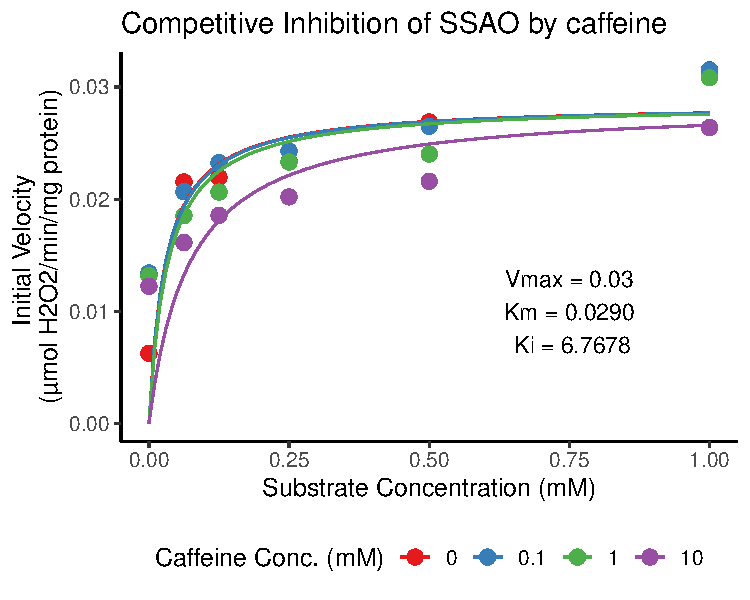
\includegraphics{results_files/figure-pdf/fig-CAF-CI-1.pdf}

}

\caption{\label{fig-CAF-CI}SSAO inhibition by caffeine, calculated by
non-linear competetive inhibition model.}

\end{figure}%

\begin{Shaded}
\begin{Highlighting}[]
\NormalTok{caf\_ssao\_nlm\_results }\OtherTok{\textless{}{-}} \FunctionTok{tibble}\NormalTok{(}\AttributeTok{Parameters\_CAF\_SSAO =} \FunctionTok{c}\NormalTok{(}\StringTok{"Km"}\NormalTok{, }\StringTok{"Vmax"}\NormalTok{, }\StringTok{"Ki"}\NormalTok{, }\StringTok{"R{-}squared"}\NormalTok{), }
                               \AttributeTok{Values =}\NormalTok{ caf\_nlm\_values)}
\FunctionTok{kable}\NormalTok{(caf\_ssao\_nlm\_results)}
\end{Highlighting}
\end{Shaded}

\begin{longtable}[]{@{}ll@{}}

\toprule\noalign{}
Parameters\_CAF\_SSAO & Values \\
\midrule\noalign{}
\endhead
\bottomrule\noalign{}
\endlastfoot
Km & 0.02903 \\
Vmax & 0.02850 \\
Ki & 6.76781 \\
R-squared & 0.28889 \\

\caption{\label{tbl-nlm-caf-fit}Non linear fit parameters for SSAO
inhibition by caffeine}

\tabularnewline

\end{longtable}

\bookmarksetup{startatroot}

\chapter{Discussion}\label{discussion}

SSAO has been studied in various cells and tissue groups that include
smooth muscle cells, intestinal tissue, heart, lungs, white adipose
tissue, brown adipose tissue, kidney, retina and placenta in models such
as mice, rats, and rabbits (Abella et al. 2003; BARRAND, FOX, and
CALLINGHAM 1984; Barrant and Callingham 1984; María Carmen Iglesias-Osma
et al. 2004; C. Li et al. 2019; Manasieva et al. 2022, 2023; Wang et al.
2018). SSAO has been detected in various tissue types in the human body
as it is widely distributed in the form of serum SSAO/VAP-1 or membrane
bound SSAO (Dunkel et al. 2008).

Membrane bound SSAO are found in adipose tissues, and vascular smooth
muscle endothelial cells in rats, mice and humans. Brown adipose tissues
were chosen to be the source of SSAO for this project to support
effective use of tissues extracted from rats. A major challenge in
extracting proteins and enzymes from adipose tissues is the higher
concentration of lipids. Hence methods that propose to remove the fat
from adipose tissues were identified and modified to fit the objectives
of the experiments. The key steps used to successfully extract SSAO
were, defatting the tissues with ethanol and dissolving the proteins in
PBS with a pH of 8.0.

Method A involved rehydrating the tissues using a freeze-dryer.
Dehydrating prior to defatting the tissues were ideal as the water
present in the tissues is miscible with ethanol, this can lead to loss
of proteins while defatting the tissues.

BCA and Bradford results for protein concentrations obtained by each
method were compared to identify a suitable method with highest quantity
of proteins. Experiment 1 of method B produced a 6.5 mg protein/ml by
BCA assay. Protein concentration estimated by BCA was considered for
downstream calculations as BCA is relatively more sensitive than
Bradford (Noble and Bailey 2009). An advantage with BCA is that it
possesses a higher tolerance for interfering species (Noble and Bailey
2009).

Method A was not repeated due to freeze dryer unavailability for
dehydration. Hence only one independent experiment was performed by
method A. Method A also produced a more efficient fat removal with
57.3\% loss in weight owing to fat and water. Method B and C were not
dehydrated before defatting, which is the potential cause for a lower
fat loss percentage with 38.7\% and 28.7\% respectively. PBS with pH 8.0
was used to dissolve the proteins as SSAO is highly stable at an optimum
pH of 8.0 and the water in the buffer dissolves the proteins present in
the tissue (Stevanato et al. 2011). While the samples were treated with
PBS, a lower temperature was maintained to prevent loss of protein
activity.~ Method C involved using a tissue homogeniser, which is prone
to generate heat when grinding the tissue. Hence, the homogenisation
setup was modified to hold the tissues in an ice bath while homogenising
at lower speeds. The tissues were homogenised with PBS instead of a
lysis buffer like RIPA to keep the buffer uniform across all methods.
The RIPA buffer contains higher concentrations of surfactants which can
potentially hinder assays such as Bradford (Noble and Bailey 2009). The
average estimated protein concentration of the extract obtained from
method C was 5.43 mg/ml and 5.27 mg/ml by Bradford and BCA assays
respectively. The extract obtained by method C had no significant SSAO
activity with 0.016554 µmol H\textsubscript{2}O\textsubscript{2} /mg
protein. In contrast, extracts obtained in experiment 1 by methods A and
B produced 2.018 and 1.641 µmol H\textsubscript{2}O\textsubscript{2}/mg
protein SSAO levels respectively. Method B was chosen to perform further
enzyme kinetic experiments. The SSAO activities measured by Amplex
\textsuperscript{®} red are corrected to per mg protein levels
calculated from BCA. After the preliminary results from experiment 1,
two more independent experiments were performed by method B and method
C. The protein concentration estimates by Bradford and BCA assays were
closer to results from experiment 1. This was also the case for SSAO
level measurements in extracts from methods B and C. Since extracts
obtained by method C did not have viable SSAO activity, the extract
obtained from method B was used for further analysis. In comparing the
quantity of proteins extracted by other methods (Bioprotocol, CST, and
RELi) with method A, method B and method C, the protocols from the
literature show significantly higher quantities than the methods used in
this project Figure~\ref{fig-protein_extraction_comparision}. The
protocols from the literature use Mice BAT for extracting proteins.
Hence to provide a fair comparison in protocols, samples from the same
animal needs to be used.

\begin{Shaded}
\begin{Highlighting}[]
\FunctionTok{library}\NormalTok{(tidyverse)}

\NormalTok{comp\_table }\OtherTok{\textless{}{-}} \FunctionTok{tibble}\NormalTok{(}\AttributeTok{Replicate =} \FunctionTok{fct}\NormalTok{(}\FunctionTok{c}\NormalTok{(}\StringTok{"1"}\NormalTok{, }\StringTok{"2"}\NormalTok{, }\StringTok{"3"}\NormalTok{, }\StringTok{"4"}\NormalTok{)),}
       \AttributeTok{Bioprotocol =} \FunctionTok{c}\NormalTok{(}\FloatTok{0.04115}\NormalTok{, }\FloatTok{0.0431}\NormalTok{, }\FloatTok{0.0374}\NormalTok{, }\FloatTok{0.04}\NormalTok{),}
       \AttributeTok{CST =} \FunctionTok{c}\NormalTok{(}\FloatTok{0.04892}\NormalTok{, }\FloatTok{0.08024}\NormalTok{, }\FloatTok{0.068}\NormalTok{, }\ConstantTok{NA}\NormalTok{),}
       \AttributeTok{RELi =} \FunctionTok{c}\NormalTok{(}\FloatTok{0.054944}\NormalTok{, }\FloatTok{0.037152}\NormalTok{, }\FloatTok{0.034784}\NormalTok{, }\ConstantTok{NA}\NormalTok{),}
       \AttributeTok{Method\_A =} \FunctionTok{c}\NormalTok{(}\FloatTok{0.004167}\NormalTok{, }\ConstantTok{NA}\NormalTok{, }\ConstantTok{NA}\NormalTok{, }\ConstantTok{NA}\NormalTok{),}
       \AttributeTok{Method\_B =} \FunctionTok{c}\NormalTok{(}\FloatTok{0.006743}\NormalTok{, }\FloatTok{0.006328}\NormalTok{, }\FloatTok{0.006432}\NormalTok{, }\ConstantTok{NA}\NormalTok{),}
       \AttributeTok{Method\_C =} \FunctionTok{c}\NormalTok{(}\FloatTok{0.005268}\NormalTok{, }\FloatTok{0.004878}\NormalTok{, }\FloatTok{0.005756}\NormalTok{, }\ConstantTok{NA}\NormalTok{)}
\NormalTok{       )}

\NormalTok{comp\_table }\SpecialCharTok{|\textgreater{}} 
  \FunctionTok{pivot\_longer}\NormalTok{(}
    \AttributeTok{cols =} \SpecialCharTok{!}\NormalTok{Replicate,}
    \AttributeTok{names\_to =} \StringTok{"Protocol"}\NormalTok{,}
    \AttributeTok{values\_to =} \StringTok{"Protein\_Estimate"}
\NormalTok{  ) }\SpecialCharTok{|\textgreater{}} \FunctionTok{group\_by}\NormalTok{(Protocol) }\SpecialCharTok{|\textgreater{}} \FunctionTok{summarise}\NormalTok{(}\AttributeTok{mean =} \FunctionTok{mean}\NormalTok{(Protein\_Estimate, }\AttributeTok{na.rm =} \ConstantTok{TRUE}\NormalTok{)) }\SpecialCharTok{|\textgreater{}} 
  \FunctionTok{ggplot}\NormalTok{(}\FunctionTok{aes}\NormalTok{(}\AttributeTok{x =} \FunctionTok{fct\_reorder}\NormalTok{(Protocol, }\FunctionTok{desc}\NormalTok{(mean)), }
             \AttributeTok{y =}\NormalTok{ mean, }\AttributeTok{fill =}\NormalTok{ Protocol))}\SpecialCharTok{+}
  \FunctionTok{geom\_bar}\NormalTok{(}\AttributeTok{stat =} \StringTok{"identity"}\NormalTok{, }
           \AttributeTok{na.rm =} \ConstantTok{FALSE}\NormalTok{, }
           \AttributeTok{orientation =} \StringTok{"x"}\NormalTok{,}
           \AttributeTok{show.legend =} \ConstantTok{FALSE}\NormalTok{)}\SpecialCharTok{+}
    \FunctionTok{geom\_text}\NormalTok{(}\FunctionTok{aes}\NormalTok{(}\AttributeTok{label =} \FunctionTok{round}\NormalTok{(mean, }\DecValTok{4}\NormalTok{)),}
    \AttributeTok{vjust =} \SpecialCharTok{{-}}\FloatTok{0.5}\NormalTok{,}
    \AttributeTok{position =} \FunctionTok{position\_dodge}\NormalTok{(}\AttributeTok{width =} \FloatTok{0.9}\NormalTok{),}
    \AttributeTok{size =} \DecValTok{3}\NormalTok{)}\SpecialCharTok{+}
  \FunctionTok{labs}\NormalTok{(}
    \AttributeTok{x =} \ConstantTok{NULL}\NormalTok{,}
    \AttributeTok{y =} \StringTok{"Average Protein Conc. }\SpecialCharTok{\textbackslash{}n}\StringTok{ (mg/ml/mg BAT/ml Buffer)"}
\NormalTok{  )}\SpecialCharTok{+}
  \FunctionTok{theme\_classic}\NormalTok{()}
\end{Highlighting}
\end{Shaded}

\begin{figure}[H]

\centering{

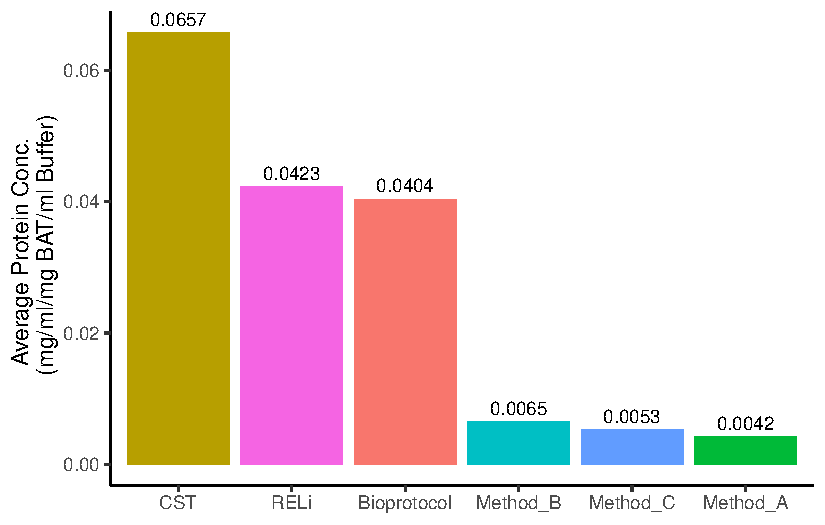
\includegraphics{discussion_files/figure-pdf/fig-protein_extraction_comparision-1.pdf}

}

\caption{\label{fig-protein_extraction_comparision}Comparison of protein
extracted by different methods in literature with methods used in this
study. The protein concentration measured by BCA is plotted in mg/ml/mg
BAT/ml buffer used (An \& Scherer, 2020; Diaz Marin et al., 2019).}

\end{figure}%

\begin{Shaded}
\begin{Highlighting}[]
\FunctionTok{library}\NormalTok{(knitr)}
\FunctionTok{kable}\NormalTok{(comp\_table)}
\end{Highlighting}
\end{Shaded}

\begin{longtable}[]{@{}
  >{\raggedright\arraybackslash}p{(\columnwidth - 12\tabcolsep) * \real{0.1515}}
  >{\raggedleft\arraybackslash}p{(\columnwidth - 12\tabcolsep) * \real{0.1818}}
  >{\raggedleft\arraybackslash}p{(\columnwidth - 12\tabcolsep) * \real{0.1212}}
  >{\raggedleft\arraybackslash}p{(\columnwidth - 12\tabcolsep) * \real{0.1364}}
  >{\raggedleft\arraybackslash}p{(\columnwidth - 12\tabcolsep) * \real{0.1364}}
  >{\raggedleft\arraybackslash}p{(\columnwidth - 12\tabcolsep) * \real{0.1364}}
  >{\raggedleft\arraybackslash}p{(\columnwidth - 12\tabcolsep) * \real{0.1364}}@{}}

\toprule\noalign{}
\begin{minipage}[b]{\linewidth}\raggedright
Replicate
\end{minipage} & \begin{minipage}[b]{\linewidth}\raggedleft
Bioprotocol
\end{minipage} & \begin{minipage}[b]{\linewidth}\raggedleft
CST
\end{minipage} & \begin{minipage}[b]{\linewidth}\raggedleft
RELi
\end{minipage} & \begin{minipage}[b]{\linewidth}\raggedleft
Method\_A
\end{minipage} & \begin{minipage}[b]{\linewidth}\raggedleft
Method\_B
\end{minipage} & \begin{minipage}[b]{\linewidth}\raggedleft
Method\_C
\end{minipage} \\
\midrule\noalign{}
\endhead
\bottomrule\noalign{}
\endlastfoot
1 & 0.04115 & 0.04892 & 0.054944 & 0.004167 & 0.006743 & 0.005268 \\
2 & 0.04310 & 0.08024 & 0.037152 & NA & 0.006328 & 0.004878 \\
3 & 0.03740 & 0.06800 & 0.034784 & NA & 0.006432 & 0.005756 \\
4 & 0.04000 & NA & NA & NA & NA & NA \\

\caption{\label{tbl-protein_comparision}A comparision of the amount of
protein (mg/ml/mg BAT/ml) extracted from BAT by different methods in the
literature and the methods used in this project}

\tabularnewline

\end{longtable}

Since there are no published methods for extracting SSAO from brown
adipose tissues in rats, the results of this study cannot be compared to
estimate correlations.

Comparative analysis using parametric or non-parametric tests was not
performed due to the limited number of experiments. Performing
statistical tests with such a small sample size would likely increase
the margin of error and reduce the confidence in the results. Therefore,
the findings were only tabulated and plotted to clearly present the
outcomes obtained in this study.

\textbf{SSAO Kinetics:}

The Km values for benzylamine as a substrate for SSAO extracted from
various species have been reported in the literature (Yraola et al.
2007). Since this study uses rats - \emph{Rattus Norvegicus} as the
source of SSAO, the results obtained are compared with Km values
estimated from same species of sample source. A study by Yraola et al
has reported a Km value of 0.0127 mM for benzylamine as a substrate for
SSAO obtained from rats (Yraola et al. 2007). This correlates with the
\textbf{Km value of 0.03193 mM} obtained from this study for benzylamine
as a substrate of SSAO obtained from rat brown adipose tissue (Yraola et
al. 2007). Moreover, the same brown adipose tissue was used by both the
studies to extract the SSAO enzyme.

Ki values for Caffeine or Simvastatin have not been reported on brown
adipose tissue SSAO obtained from \emph{Rattus Norvegicus.} This study
is the first to report the Ki values from caffeine and simvastatin on
SSAO obtained from rats. However, a study by Sun P et al., has reported
that simvastatin has reduced the release of membrane bound SSAO into
circulation and thus preventing leukocyte adhesion and OGD mediated
increase in vascular permeability (Sun et al. 2018). This study by Sun
et al., measures the levels of SSAO by western blotting and does not
provide a Ki value for simvastatin. A study by Che et al., reported that
administration of caffeine to male Wistar rats caused a reduction in
SSAO quantities due to accumulation of caffeine (Che et al. 2012). But
no Ki values have been reported in the literature. \textbf{The Ki values
obtained from this project are 2.145 and 6.768 mM for simvastatin and
caffeine respectively.} The Ki values obtained are outside the inhibitor
concentration range used to calculate them, indicating a need to repeat
the inhibition experiments with updated concentrations that reflect the
current Ki values. The fact that these Ki values fall within the
millimolar range suggests that both compounds are not potent inhibitors
of SSAO.

However, it's important to note that these results are based on a single
independent experiment. Additionally, this study did not use inhibitors
with known Ki values as controls, which limits the ability to accurately
compare the inhibition effects of different compounds. Future research
should focus on addressing these limitations to improve accuracy and
reduce errors, leading to more reliable results.

\bookmarksetup{startatroot}

\chapter{Limitations and future
works}\label{limitations-and-future-works}

\begin{enumerate}
\def\labelenumi{\arabic{enumi}.}
\tightlist
\item
  To analyse the extract from rat BAT for more specificity of substrates
  to distinguish the type of SSAO present. This can be achieved by
  comparing the reaction rates by using different substrates such as
  tyramine and benzylamine along with known inhibitors of other classes
  of deamination enzymes such as the monoamine oxidases (MAO - A and MAO
  - B).
\item
  Reanalyse the inhibition properties of simvastatin and caffeine with
  additional controls such as inhibitors such as the MDL72794A,
  PXS-4728A, methylhydrazine and semi carbazide. This could potentially
  increase the reliability of the inhibition kinetic results.
  Optimisation of inhibitor concentrations to reevaluate the Ki for
  simvastatin and caffeine.
\item
  Conduct a larger number of independent experiments to enhance the
  confidence interval and reduce error.
\item
  No subsequent assays were performed to verify complete elimination of
  fats by any of the methods used.
\item
  The extracts were stored at -20℃ instead of -80℃ (standard practice),
  which could have affected the stability of the enzymes present in the
  extracts leading to a reduced activity.
\end{enumerate}

\bookmarksetup{startatroot}

\chapter{Conclusion}\label{conclusion}

This study presents a comprehensive methodology for extracting SSAO from
rat brown adipose tissues, demonstrating effective protein
quantification through Bradford and BCA assays, even after defatting
with 100\% ethanol. Despite storage at -20°C, the samples retained
quantifiable SSAO activity, as measured by the Amplex\textsuperscript{®}
Red monoamine oxidase assay. The kinetic parameters obtained for SSAO,
with a Km of 0.03193 using benzylamine as a substrate, align closely
with previously published results under similar conditions.

However, the Ki values for caffeine and simvastatin were derived from a
single experiment, leading to a wider error margin and lower confidence
in these results. Additionally, these Ki values fall within the
millimolar range, suggesting that both compounds may not be potent
inhibitors of SSAO. It is also worth noting that these values were
outside the inhibitor concentration range used in their calculation,
indicating a need for repeated experiments with adjusted concentrations
that reflect the current Ki values. Moreover, the absence of inhibitors
with known Ki values as controls limits the ability to accurately
compare the inhibition effects of different compounds.

In conclusion, while the study successfully establishes a reliable
method for SSAO extraction and activity measurement, further experiments
with improved controls and optimized conditions are necessary to yield
more reliable Ki values for caffeine and simvastatin. Addressing these
limitations in future research will enhance the accuracy and robustness
of the findings.

\bookmarksetup{startatroot}

\chapter*{References}\label{references}
\addcontentsline{toc}{chapter}{References}

\markboth{References}{References}

\phantomsection\label{refs}
\begin{CSLReferences}{1}{0}
\bibitem[\citeproctext]{ref-Copeland.R.A.2005}
A., Copeland R. 2005. {``Evaluation of Enzyme Inhibitors in Drug
Discovery. A Guide for Medicinal Chemists and Pharmacologists.''}
\emph{Methods of Biochemical Analysis} 46: 1--265.

\bibitem[\citeproctext]{ref-Abella2003}
Abella, Anna, Luc Marti, Marta Camps, Marc Claret, J. Fernández-Alvarez,
Ramon Gomis, Anna Gumà, et al. 2003. {``Semicarbazide-Sensitive Amine
Oxidase/Vascular Adhesion Protein-1 Activity Exerts an Antidiabetic
Action in Goto-Kakizaki Rats.''} \emph{Diabetes} 52 (April): 1004--13.
\url{https://doi.org/10.2337/DIABETES.52.4.1004}.

\bibitem[\citeproctext]{ref-An2020}
An, Yu A., and Philipp E. Scherer. 2020. {``Mouse Adipose Tissue Protein
Extraction.''} \emph{Bio-Protocol} 10 (June).
\url{https://doi.org/10.21769/BIOPROTOC.3631}.

\bibitem[\citeproctext]{ref-Arvilommi1997}
Arvilommi, Anna Maija, Marko Salmi, and Sirpa Jalkanen. 1997.
{``Organ-Selective Regulation of Vascular Adhesion Protein-1 Expression
in Man.''} \emph{European Journal of Immunology} 27 (July): 1794--1800.
\url{https://doi.org/10.1002/EJI.1830270730}.

\bibitem[\citeproctext]{ref-BARRAND1984}
BARRAND, MARGERY A., SHEILA A. FOX, and BRIAN A. CALLINGHAM. 1984.
{``Amine Oxidase Activities in Brown Adipose Tissue of the Rat:
Identification of Semicarbazide‐sensitive (Clorgyline‐resistant)
Activity at the Fat Cell Membrane.''} \emph{Journal of Pharmacy and
Pharmacology} 36: 652--58.
\url{https://doi.org/10.1111/j.2042-7158.1984.tb04837.x}.

\bibitem[\citeproctext]{ref-Barrant1984}
Barrant, M. A., and B. A. Callingham. 1984. {``Solubilization and Some
Properties of a Semicarbazide-Sensitive Amine Oxidase in Brown Adipose
Tissue of the Rat.''} \emph{The Biochemical Journal} 222: 467--75.
\url{https://doi.org/10.1042/BJ2220467}.

\bibitem[\citeproctext]{ref-Belligoli2019}
Belligoli, Anna, Chiara Compagnin, Marta Sanna, Francesca Favaretto,
Roberto Fabris, Luca Busetto, Mirto Foletto, et al. 2019.
{``Characterization of Subcutaneous and Omental Adipose Tissue in
Patients with Obesity and with Different Degrees of Glucose
Impairment.''} \emph{Scientific Reports} 9 (August): 11333.
\url{https://doi.org/10.1038/S41598-019-47719-Y}.

\bibitem[\citeproctext]{ref-Blondin2020}
Blondin, Denis P., Soren Nielsen, Eline N. Kuipers, Mai C. Severinsen,
Verena H. Jensen, Stéphanie Miard, Naja Z. Jespersen, et al. 2020.
{``Human Brown Adipocyte Thermogenesis Is Driven by Β2-AR
Stimulation.''} \emph{Cell Metabolism} 32 (August): 287--300.e7.
\url{https://doi.org/10.1016/J.CMET.2020.07.005}.

\bibitem[\citeproctext]{ref-Boomsma2000}
Boomsma, F., P. J. De Kam, G. Tjeerdsma, A. H. Van Den Meiracker, and D.
J. Van Veldhuisen. 2000. {``Plasma Semicarbazide-Sensitive Amine Oxidase
(SSAO) Is an Independent Prognostic Marker for Mortality in Chronic
Heart Failure.''} \emph{European Heart Journal} 21: 1859--63.
\url{https://doi.org/10.1053/EUHJ.2000.2176}.

\bibitem[\citeproctext]{ref-Buxf6rgeson2022}
Börgeson, Emma, Jeremie Boucher, and Carolina E. Hagberg. 2022. {``Of
Mice and Men: Pinpointing Species Differences in Adipose Tissue
Biology.''} \emph{Frontiers in Cell and Developmental Biology} 10
(September): 1003118.
\url{https://doi.org/10.3389/FCELL.2022.1003118/BIBTEX}.

\bibitem[\citeproctext]{ref-Bour2009}
Bour, Sandy, Sylvie Caspar-Bauguil, Zsuzsa Iffiú-Soltész, Maryse
Nibbelink, Béatrice Cousin, Mari Miiluniemi, Marko Salmi, et al. 2009.
{``Semicarbazide-Sensitive Amine Oxidase/Vascular Adhesion Protein-1
Deficiency Reduces Leukocyte Infiltration into Adipose Tissue and Favors
Fat Deposition.''} \emph{The American Journal of Pathology} 174:
1075--83. \url{https://doi.org/10.2353/AJPATH.2009.080612}.

\bibitem[\citeproctext]{ref-Cai2022}
Cai, Limeng, Yuqi Wang, Ying Yang, and Hao Wu. 2022. {``A Low-Cost,
Enzyme-Coupled Fluorescent Assay for Rapid Quantification of Glycolysis
Rate of Cells.''} \emph{Analytical and Bioanalytical Chemistry} 414
(February): 1987--97.
\url{https://doi.org/10.1007/S00216-021-03834-2/METRICS}.

\bibitem[\citeproctext]{ref-Carpuxe9nuxe92019}
Carpéné, Christian, Nathalie Boulet, Alice Chaplin, and Josep Mercader.
2019. {``Past, Present and Future Anti-Obesity Effects of
Flavin-Containing and/or Copper-Containing Amine Oxidase Inhibitors.''}
\emph{Medicines (Basel, Switzerland)} 6 (January): 9.
\url{https://doi.org/10.3390/MEDICINES6010009}.

\bibitem[\citeproctext]{ref-Chait2020}
Chait, Alan, and Laura J. den Hartigh. 2020. {``Adipose Tissue
Distribution, Inflammation and Its Metabolic Consequences, Including
Diabetes and Cardiovascular Disease.''} \emph{Frontiers in
Cardiovascular Medicine} 7 (February).
\url{https://doi.org/10.3389/FCVM.2020.00022}.

\bibitem[\citeproctext]{ref-Che2012}
Che, Baoquan, Lin Wang, Zhe Zhang, Yongqian Zhang, and Yulin Deng. 2012.
{``Distribution and Accumulation of Caffeine in Rat Tissues and Its
Inhibition on Semicarbazide-Sensitive Amine Oxidase.''}
\emph{NeuroToxicology} 33 (October): 1248--53.
\url{https://doi.org/10.1016/J.NEURO.2012.07.004}.

\bibitem[\citeproctext]{ref-Chew2023}
Chew, Nicholas W. S., Cheng Han Ng, Darren Jun Hao Tan, Gwyneth Kong,
Chaoxing Lin, Yip Han Chin, Wen Hui Lim, et al. 2023. {``The Global
Burden of Metabolic Disease: Data from 2000 to 2019.''} \emph{Cell
Metabolism} 35 (March): 414--428.e3.
\url{https://doi.org/10.1016/j.cmet.2023.02.003}.

\bibitem[\citeproctext]{ref-Chusyd2016}
Chusyd, Daniella E., Donghai Wang, Derek M. Huffman, and Tim R. Nagy.
2016. {``Relationships Between Rodent White Adipose Fat Pads and Human
White Adipose Fat Depots.''} \emph{Frontiers in Nutrition} 3 (April).
\url{https://doi.org/10.3389/FNUT.2016.00010}.

\bibitem[\citeproctext]{ref-Danielli2022}
Danielli, Marianna, Roisin Clare Thomas, Lauren Marie Quinn, and Bee
Kang Tan. 2022. {``Vascular Adhesion Protein-1 (VAP-1) in Vascular
Inflammatory Diseases: A Narrative Review.''} \emph{Vasa - European
Journal of Vascular Medicine} 51 (November): 341--50.
\url{https://doi.org/10.1024/0301-1526/a001031}.

\bibitem[\citeproctext]{ref-Dezse2020}
Dezse, K. E., W. P. Frank, and C. A. C. Baptista. 2020. {``Fat Removal
During Acetone Dehydration and Defatting Phases of Plastination.''}
\emph{Journal of Plastination} 32: 26--30.
\url{https://doi.org/10.56507/MBJO3692}.

\bibitem[\citeproctext]{ref-Dunkel2008}
Dunkel, P., A. Gelain, D. Barlocco, N. Haider, K. Gyires, B. Sperlagh,
K. Magyar, E. Maccioni, A. Fadda, and P. Matyus. 2008.
{``Semicarbazide-Sensitive Amine Oxidase/Vascular Adhesion Protein 1:
Recent Developments Concerning Substrates and Inhibitors of a Promising
Therapeutic Target.''} \emph{Current Medicinal Chemistry} 15 (July):
1827--39. \url{https://doi.org/10.2174/092986708785133022}.

\bibitem[\citeproctext]{ref-Hernandez-Guillamon2010}
Hernandez-Guillamon, Mar, Lidia Garcia-Bonilla, Montse Solé, Victoria
Sosti, Mireia Parés, Mireia Campos, Arantxa Ortega-Aznar, et al. 2010.
{``Plasma VAP-1/SSAO Activity Predicts Intracranial Hemorrhages and
Adverse Neurological Outcome After Tissue Plasminogen Activator
Treatment in Stroke.''} \emph{Stroke} 41: 1528--35.
\url{https://doi.org/10.1161/STROKEAHA.110.584623}.

\bibitem[\citeproctext]{ref-Iglesias-Osma2005}
Iglesias-Osma, Maria Carmen, Sandy Bour, Maria Jose Garcia-Barrado,
Virgile Visentin, Maria Francisca Pastor, Xavier Testar, Luc Marti, et
al. 2005. {``Methylamine but Not Mafenide Mimics Insulin-Like Activity
of the Semicarbazide-Sensitive Amine Oxidase-Substrate Benzylamine on
Glucose Tolerance and on Human Adipocyte Metabolism.''}
\emph{Pharmacological Research} 52 (December): 475--84.
\url{https://doi.org/10.1016/J.PHRS.2005.07.008}.

\bibitem[\citeproctext]{ref-Iglesias-Osma2004}
Iglesias-Osma, María Carmen, Maria José Garcia-Barrado, Virgile
Visentin, Maria Francisca Pastor-Mansilla, Sandy Bour, Daníelle Prévot,
Philippe Valet, Julio Moratinos, and Christian Carpéné. 2004.
{``Benzylamine Exhibits Insulin-Like Effects on Glucose Disposal,
Glucose Transport, and Fat Cell Lipolysis in Rabbits and Diabetic
Mice.''} \emph{The Journal of Pharmacology and Experimental
Therapeutics} 309 (June): 1020--28.
\url{https://doi.org/10.1124/JPET.103.063636}.

\bibitem[\citeproctext]{ref-Jarnicki2016}
Jarnicki, A. G., H. Schilter, G. Liu, K. Wheeldon, A. T. Essilfie, J. S.
Foot, T. T. Yow, W. Jarolimek, and Philip M. Hansbro. 2016. {``The
Inhibitor of Semicarbazide-Sensitive Amine Oxidase, PXS-4728A,
Ameliorates Key Features of Chronic Obstructive Pulmonary Disease in a
Mouse Model.''} \emph{British Journal of Pharmacology} 173: 3161--75.
\url{https://doi.org/10.1111/bph.13573}.

\bibitem[\citeproctext]{ref-Karakuzu2019}
Karakuzu, Ozgur, Melissa R. Cruz, Yi Liu, and Danielle A. Garsin. 2019.
{``Amplex Red Assay for Measuring Hydrogen Peroxide Production from
Caenorhabditis Elegans.''} \emph{Bio-Protocol} 9 (November).
\url{https://doi.org/10.21769/BIOPROTOC.3409}.

\bibitem[\citeproctext]{ref-Kurkijarvi2000}
Kurkijarvi, Riikka, Gennady G. Yegutkin, Bridget K. Gunson, Sirpa
Jalkanen, Marko Salmi, and David H. Adams. 2000. {``Circulating Soluble
Vascular Adhesion Protein 1 Accounts for the Increased Serum Monoamine
Oxidase Activity Chronic Liver Disease.''} \emph{Gastroenterology} 119:
1096--1103. \url{https://doi.org/10.1053/gast.2000.18163}.

\bibitem[\citeproctext]{ref-Li2019}
Li, Chaosheng, Zhenhua Wang, Xiaoli Li, and Jun Chen. 2019. {``Effects
of Semicarbazide-Sensitive Amine Oxidase Inhibitors on Morphology of
Aorta and Kidney in Diabetic Rats.''} \emph{BMC Endocrine Disorders} 19
(June). \url{https://doi.org/10.1186/S12902-019-0392-1}.

\bibitem[\citeproctext]{ref-Li2021}
Li, Hui, Shiyu Du, Panpan Niu, Xiaosong Gu, Jun Wang, and Ying Zhao.
2021. {``Vascular Adhesion Protein-1 (VAP-1)/Semicarbazide-Sensitive
Amine Oxidase (SSAO): A Potential Therapeutic Target for Atherosclerotic
Cardiovascular Diseases.''} \emph{Frontiers in Pharmacology} 12 (July).
\url{https://doi.org/10.3389/FPHAR.2021.679707}.

\bibitem[\citeproctext]{ref-Lyles1995}
Lyles, G. A. 1995. {``Substrate-Specificity of Mammalian Tissue-Bound
Semicarbazide-Sensitive Amine Oxidase.''} \emph{Progress in Brain
Research} 106: 293--303.
\url{https://doi.org/10.1016/s0079-6123(08)61226-1}.

\bibitem[\citeproctext]{ref-Ma2011}
Ma, Qingyi, Anatol Manaenko, Nikan H. Khatibi, Wanqiu Chen, John H.
Zhang, and Jiping Tang. 2011. {``Vascular Adhesion Protein-1 Inhibition
Provides Antiinflammatory Protection After an Intracerebral Hemorrhagic
Stroke in Mice.''} \emph{Journal of Cerebral Blood Flow and Metabolism :
Official Journal of the International Society of Cerebral Blood Flow and
Metabolism} 31: 881--93. \url{https://doi.org/10.1038/JCBFM.2010.167}.

\bibitem[\citeproctext]{ref-Manasieva2023}
Manasieva, Vesna, Shori Thakur, Lisa A. Lione, Anwar R. Baydoun, and
John Skamarauskas. 2023. {``The Impact of Semicarbazide Sensitive Amine
Oxidase Activity on Rat Aortic Vascular Smooth Muscle Cells.''}
\emph{International Journal of Molecular Sciences 2023, Vol. 24, Page
4946} 24 (March): 4946. \url{https://doi.org/10.3390/IJMS24054946}.

\bibitem[\citeproctext]{ref-Manasieva2022}
Manasieva, Vesna, Shori Thakur, Lisa A. Lione, Jessal Patel, Anwar
Baydoun, and John Skamarauskas. 2022. {``Semicarbazide-Sensitive Amine
Oxidase (SSAO) and Lysyl Oxidase (LOX) Association in Rat Aortic
Vascular Smooth Muscle Cells.''} \emph{Biomolecules} 12 (November).
\url{https://doi.org/10.3390/BIOM12111563}.

\bibitem[\citeproctext]{ref-Marin2019}
Marin, R. Diaz, S. Crespo-Garcia, Ariel Molly Wilson, and P. Sapieha.
2019. {``RELi Protocol: Optimization for Protein Extraction from White,
Brown and Beige Adipose Tissues.''} \emph{MethodsX} 6 (January):
918--28. \url{https://doi.org/10.1016/J.MEX.2019.04.010}.

\bibitem[\citeproctext]{ref-Mercader2011}
Mercader, Josep, Zsuzsa Iffiú-Soltész, Sandy Bour, and Christian
Carpéné. 2011. {``Oral Administration of Semicarbazide Limits Weight
Gain Together with Inhibition of Fat Deposition and of Primary Amine
Oxidase Activity in Adipose Tissue.''} \emph{Journal of Obesity} 2011
(January): 475786. \url{https://doi.org/10.1155/2011/475786}.

\bibitem[\citeproctext]{ref-Murata2017}
Murata, Miyuki, Kousuke Noda, Akiko Kawasaki, Shiho Yoshida, Yoko Dong,
Michiyuki Saito, Zhenyu Dong, et al. 2017. {``Soluble Vascular Adhesion
Protein-1 Mediates Spermine Oxidation as Semicarbazide-Sensitive Amine
Oxidase: Possible Role in Proliferative Diabetic Retinopathy.''}
\emph{Current Eye Research} 42 (December): 1674--83.
\url{https://doi.org/10.1080/02713683.2017.1359847}.

\bibitem[\citeproctext]{ref-Noble2009}
Noble, James E., and Marc J. A. Bailey. 2009. {``Chapter 8 Quantitation
of Protein.''} \emph{Methods in Enzymology} 463 (January): 73--95.
\url{https://doi.org/10.1016/S0076-6879(09)63008-1}.

\bibitem[\citeproctext]{ref-Obata2006}
Obata, Toshio. 2006. {``Diabetes and Semicarbazide-Sensitive Amine
Oxidase (SSAO) Activity: A Review.''} \emph{Life Sciences} 79 (June):
417--22. \url{https://doi.org/10.1016/j.lfs.2006.01.017}.

\bibitem[\citeproctext]{ref-Pannecoeck2015}
Pannecoeck, Roos, Daphne Serruys, Lara Benmeridja, Joris R. Delanghe,
Nanja Van Geel, Reinhart Speeckaert, and Marijn M. Speeckaert. 2015.
{``Vascular Adhesion Protein-1: Role in Human Pathology and Application
as a Biomarker.''} \emph{Critical Reviews in Clinical Laboratory
Sciences} 52: 284--300.
\url{https://doi.org/10.3109/10408363.2015.1050714}.

\bibitem[\citeproctext]{ref-Papukashvili2020}
Papukashvili, Dimitri, Nino Rcheulishvili, and Yulin Deng. 2020.
{``Attenuation of Weight Gain and Prevention of Associated Pathologies
by Inhibiting SSAO.''} \emph{Nutrients} 12.
\url{https://doi.org/10.3390/NU12010184}.

\bibitem[\citeproctext]{ref-Peng2016}
Peng, Ya, Jun Wang, Miao Zhang, Panpan Niu, Mengya Yang, Yilin Yang, and
Ying Zhao. 2016. {``Inactivation of Semicarbazide-Sensitive Amine
Oxidase Stabilizes the Established Atherosclerotic Lesions via Inducing
the Phenotypic Switch of Smooth Muscle Cells.''} \emph{PloS One} 11
(April). \url{https://doi.org/10.1371/JOURNAL.PONE.0152758}.

\bibitem[\citeproctext]{ref-Reddy2024}
Reddy, Vundrala Sumedha, S. Shiva, Srinidhi Manikantan, and Seeram
Ramakrishna. 2024. {``Pharmacology of Caffeine and Its Effects on the
Human Body.''} \emph{European Journal of Medicinal Chemistry Reports} 10
(April): 100138. \url{https://doi.org/10.1016/J.EJMCR.2024.100138}.

\bibitem[\citeproctext]{ref-Salmi1992}
Salmi, Marko, and Sirpa Jalkanen. 1992. {``A 90-Kilodalton Endothelial
Cell Molecule Mediating Lymphocyte Binding in Humans.''} \emph{Science
(New York, N.Y.)} 257 (September): 1407--9.
\url{https://doi.org/10.1126/SCIENCE.1529341}.

\bibitem[\citeproctext]{ref-Salmi2019}
---------. 2019. {``Vascular Adhesion Protein-1: A Cell Surface Amine
Oxidase in Translation.''} \emph{Antioxidants \& Redox Signaling} 30
(January): 314. \url{https://doi.org/10.1089/ARS.2017.7418}.

\bibitem[\citeproctext]{ref-Salmi2000}
Salmi, Marko, Sami Tohka, and Sirpa Jalkanen. 2000. {``Human Vascular
Adhesion Protein-1 (VAP-1) Plays a Critical Role in
Lymphocyte-Endothelial Cell Adhesion Cascade Under Shear.''}
\emph{Circulation Research} 86 (June): 1245--51.
\url{https://doi.org/10.1161/01.RES.86.12.1245}.

\bibitem[\citeproctext]{ref-Schilter2015}
Schilter, Heidi C., Adam Collison, Remo C. Russo, Jonathan S. Foot, Tin
T. Yow, Angelica T. Vieira, Livia D. Tavares, Joerg Mattes, Mauro M.
Teixeira, and Wolfgang Jarolimek. 2015. {``Effects of an
Anti-Inflammatory VAP-1/SSAO Inhibitor, PXS-4728A, on Pulmonary
Neutrophil Migration.''} \emph{Respiratory Research} 16 (March).
\url{https://doi.org/10.1186/S12931-015-0200-Z}.

\bibitem[\citeproctext]{ref-Silvola2016}
Silvola, Johanna M. U., Helena Virtanen, Riikka Siitonen, Sanna
Hellberg, Heidi Liljenbäck, Olli Metsälä, Mia Ståhle, et al. 2016.
{``Leukocyte Trafficking-Associated Vascular Adhesion Protein 1 Is
Expressed and Functionally Active in Atherosclerotic Plaques.''}
\emph{Scientific Reports} 6 (October).
\url{https://doi.org/10.1038/SREP35089}.

\bibitem[\citeproctext]{ref-Stevanato2011}
Stevanato, Roberto, Sara Cardillo, Michele Braga, Angela De Iuliis,
Valentina Battaglia, Antonio Toninello, Enzo Agostinelli, and Fabio
Vianello. 2011. {``Preliminary Kinetic Characterization of a Copper
Amine Oxidase from Rat Liver Mitochondria Matrix.''} \emph{Amino Acids}
40: 713--20. \url{https://doi.org/10.1007/S00726-010-0708-Y}.

\bibitem[\citeproctext]{ref-Sun2018}
Sun, Ping, Mar Hernandez-Guillamón, Mireia Campos-Martorell, Alba
Simats, Joan Montaner, Mercedes Unzeta, and Montse Solé. 2018.
{``Simvastatin Blocks Soluble SSAO/VAP-1 Release in Experimental Models
of Cerebral Ischemia: Possible Benefits for Stroke-Induced Inflammation
Control.''} \emph{Biochimica Et Biophysica Acta. Molecular Basis of
Disease} 1864 (February): 542--53.
\url{https://doi.org/10.1016/J.BBADIS.2017.11.014}.

\bibitem[\citeproctext]{ref-Tuxe1bi2013}
Tábi, Tamás, Éva Szöko, Anita Mérey, Veronika Tóth, Péter Mátyus, and
Klára Gyires. 2013. {``Study on SSAO Enzyme Activity and
Anti-Inflammatory Effect of SSAO Inhibitors in Animal Model of
Inflammation.''} \emph{Journal of Neural Transmission (Vienna, Austria :
1996)} 120 (June): 963--67.
\url{https://doi.org/10.1007/S00702-012-0961-1}.

\bibitem[\citeproctext]{ref-Toiyama2009}
Toiyama, Yuji, Chikao Miki, Yasuhiro Inoue, Aya Kawamoto, and Masato
Kusunoki. 2009. {``Circulating Form of Human Vascular Adhesion Protein-1
(VAP-1): Decreased Serum Levels in Progression of Colorectal Cancer and
Predictive Marker of Lymphatic and Hepatic Metastasis.''} \emph{Journal
of Surgical Oncology} 99 (May): 368--72.
\url{https://doi.org/10.1002/jso.21246}.

\bibitem[\citeproctext]{ref-Unzeta2021}
Unzeta, Mercedes, Mar Hernàndez-Guillamon, Ping Sun, and Montse Solé.
2021. {``SSAO/VAP-1 in Cerebrovascular Disorders: A Potential
Therapeutic Target for Stroke and Alzheimer's Disease.''}
\emph{International Journal of Molecular Sciences 2021, Vol. 22, Page
3365} 22 (March): 3365. \url{https://doi.org/10.3390/IJMS22073365}.

\bibitem[\citeproctext]{ref-Wang2018}
Wang, Shu Huei, Tse Ya Yu, Feng Chiao Tsai, Chris J. Weston, Mao Shin
Lin, Chi Sheng Hung, Hsien Li Kao, et al. 2018. {``Inhibition of
Semicarbazide-Sensitive Amine Oxidase Reduces Atherosclerosis in
Apolipoprotein e-Deficient Mice.''} \emph{Translational Research} 197
(July): 12--31. \url{https://doi.org/10.1016/j.trsl.2018.03.001}.

\bibitem[\citeproctext]{ref-Xu2014}
Xu, Hao Liang, Maggie Garcia, Fernando Testai, Francesco Vetri,
Alexandra Barabanova, Dale A. Pelligrino, and Chanannait Paisansathan.
2014. {``Pharmacologic Blockade of Vascular Adhesion Protein-1 Lessens
Neurologic Dysfunction in Rats Subjected to Subarachnoid Hemorrhage.''}
\emph{Brain Research} 1586 (October): 83--89.
\url{https://doi.org/10.1016/J.BRAINRES.2014.08.036}.

\bibitem[\citeproctext]{ref-Yan2023}
Yan, Liben, Chunli Sun, Yaxi Zhang, Peng Zhang, Yu Chen, Yifan Deng,
Tianyi Er, Yulin Deng, Zhimin Wang, and Hong Ma. 2023. {``The Biological
Implication of Semicarbazide-Sensitive Amine Oxidase (SSAO) Upregulation
in Rat Systemic Inflammatory Response Under Simulated Aerospace
Environment.''} \emph{International Journal of Molecular Sciences} 24
(February): 3666. \url{https://doi.org/10.3390/IJMS24043666/S1}.

\bibitem[\citeproctext]{ref-Yang2011}
Yang, Wei, Hui Li, Hongjun Luo, and Wenhong Luo. 2011. {``Inhibition of
Semicarbazide-Sensitive Amine Oxidase Attenuates Myocardial
Ischemia-Reperfusion Injury in an in Vivo Rat Model.''} \emph{Life
Sciences} 88 (February): 302--6.
\url{https://doi.org/10.1016/J.LFS.2010.12.003}.

\bibitem[\citeproctext]{ref-Yasuda2011}
Yasuda, Hiromi, Yuji Toiyama, Masaki Ohi, Yasuhiko Mohri, Chikao Miki,
and Masato Kusunoki. 2011. {``Serum Soluble Vascular Adhesion Protein-1
Is a Valuable Prognostic Marker in Gastric Cancer.''} \emph{Journal of
Surgical Oncology} 103 (June): 695--99.
\url{https://doi.org/10.1002/jso.21877}.

\bibitem[\citeproctext]{ref-Yraola2007}
Yraola, Francesc, Silvia García-Vicente, Luc Marti, Fernando Albericio,
Antonio Zorzano, and Miriam Royo. 2007. {``Understanding the Mechanism
of Action of the Novel SSAO Substrate (C7NH10)6(V10O28)·2H2O, a Prodrug
of Peroxovanadate Insulin Mimetics.''} \emph{Chemical Biology \& Drug
Design} 69 (June): 423--28.
\url{https://doi.org/10.1111/J.1747-0285.2007.00516.X}.

\bibitem[\citeproctext]{ref-Yu1998}
Yu, P. H., and Y. L. Deng. 1998. {``Endogenous Formaldehyde as a
Potential Factor of Vulnerability of Atherosclerosis: Involvement of
Semicarbazide-Sensitive Amine Oxidase-Mediated Methylamine Turnover.''}
\emph{Atherosclerosis} 140 (October): 357--63.
\url{https://doi.org/10.1016/S0021-9150(98)00142-7}.

\bibitem[\citeproctext]{ref-Yu2004}
Yu, Peter H., Michael Wang, Hui Fan, Yulin Deng, and Diana
Gubisne-Haberle. 2004. {``Involvement of SSAO-Mediated Deamination in
Adipose Glucose Transport and Weight Gain in Obese Diabetic KKAy
Mice.''} \emph{American Journal of Physiology - Endocrinology and
Metabolism} 286 (April).
\url{https://doi.org/10.1152/AJPENDO.00272.2003}.

\bibitem[\citeproctext]{ref-Yu2002}
Yu, P., M. Wang, Y. Deng, H. Fan, and L. Shira-Bock. 2002.
{``Involvement of Semicarbazide-Sensitive Amine Oxidase-Mediated
Deamination in Atherogenesis in KKAy Diabetic Mice Fed with High
Cholesterol Diet.''} \emph{Diabetologia} 45: 1255--62.
\url{https://doi.org/10.1007/S00125-002-0903-9}.

\bibitem[\citeproctext]{ref-Zhang2016}
Zhang, Miao, Limin Liu, Feng Zhi, Panpan Niu, Mengya Yang, Xuemei Zhu,
Ying Diao, Yanmei Li, Jun Wang, and Ying Zhao. 2016. {``Inactivation of
Semicarbazide-Sensitive Amine Oxidase Induces the Phenotypic Switch of
Smooth Muscle Cells and Aggravates the Development of Atherosclerotic
Lesions.''} \emph{Atherosclerosis} 249 (June): 76--82.
\url{https://doi.org/10.1016/J.ATHEROSCLEROSIS.2016.03.039}.

\bibitem[\citeproctext]{ref-Zorzano2003}
Zorzano, Antonio, Anna Abella, Luc Marti, Christian Carpéné, Manuel
Palacín, and Xavier Testar. 2003. {``Semicarbazide-Sensitive Amine
Oxidase Activity Exerts Insulin-Like Effects on Glucose Metabolism and
Insulin-Signaling Pathways in Adipose Cells.''} \emph{Biochimica Et
Biophysica Acta - Proteins and Proteomics} 1647 (April): 3--9.
\url{https://doi.org/10.1016/S1570-9639(03)00039-6}.

\end{CSLReferences}




\end{document}
